\documentclass[preprint,12pt,authoryear]{elsarticle}
\usepackage[letterpaper,margin=1in]{geometry}
\usepackage[UTF8,fontset=fandol,heading=false,scheme=chinese]{ctex}
\usepackage{amsmath,amssymb,amsfonts,bm}
\usepackage{graphicx}
\usepackage{longtable,booktabs,array,calc}
\usepackage{xcolor}
\usepackage{pdflscape}
\usepackage[hidelinks]{hyperref}
\usepackage{newunicodechar}
\newunicodechar{→}{\ensuremath{\rightarrow}}
\newunicodechar{⁻}{\textsuperscript{-}}
\newunicodechar{⁵}{\textsuperscript{5}}
\newunicodechar{·}{\textperiodcentered}
\newunicodechar{×}{\ensuremath{\times}}
\newunicodechar{−}{\ensuremath{-}}
\newunicodechar{⊗}{\ensuremath{\otimes}}
\newunicodechar{≤}{\ensuremath{\leq}}
\providecommand{\tightlist}{\setlength{\itemsep}{0pt}\setlength{\parskip}{0pt}}
\makeatletter
\newsavebox\pandoc@box
\newcommand*\pandocbounded[1]{\sbox\pandoc@box{#1}%
  \Gscale@div\@tempa{\textheight}{\dimexpr\ht\pandoc@box+\dp\pandoc@box\relax}%
  \Gscale@div\@tempb{\linewidth}{\wd\pandoc@box}%
  \ifdim\@tempb\p@<\@tempa\p@\let\@tempa\@tempb\fi
  \ifdim\@tempa\p@<\p@\scalebox{\@tempa}{\usebox\pandoc@box}\else\usebox{\pandoc@box}\fi}
\makeatother
\def\LTcaptype{table}
\setlength{\LTleft}{0pt}\setlength{\LTright}{0pt}\setlength{\LTcapwidth}{\linewidth}
\setlength{\emergencystretch}{3em}
\journal{Computer Methods in Applied Mechanics and Engineering}
\newunicodechar{⪯}{\ensuremath{\preceq}}\newunicodechar{⪰}{\ensuremath{\succeq}}
\newunicodechar{δ}{\ensuremath{\delta}}\newunicodechar{κ}{\ensuremath{\kappa}}
\abstracttitle{摘要}\keywordtitle{关键词}
\linespread{1.25}
\begin{document}
\begin{frontmatter}
\title{带平衡校正的神经初始化静力凝聚：切割薄壁 TPMS 格栅的分析与厚度设计}
% Author block (elsarticle). Fill in names, affiliations and the corresponding author; the build inserts this file
% into the front matter after the title. Placeholders are printed in red so that none can go out unnoticed.
\author[a]{\textcolor{red}{[First author]}\corref{cor1}}
\ead{[corresponding e-mail]}
\author[a]{\textcolor{red}{[Second author]}}
\cortext[cor1]{Corresponding author.}
\affiliation[a]{organization={\textcolor{red}{[Department, University]}},
  city={\textcolor{red}{[City]}}, country={\textcolor{red}{[Country]}}}

\begin{abstract}
由几何变化的组件构成的结构（如梯度格栅和切割格栅）规模过大，无法在每次设计变更时都完整求解，同时又缺乏均匀化所需的尺度分离：对于一层在切割面上固支的胞层，均匀化低估柔度达 27\%。精确凝聚对每一种几何都需要进行一次内部分解；学习子结构只保留少量边界自由度，而组件降基方法则依赖共享的离散空间。本文中，学习模型作用于一个离散空间随几何变化的组件的全部盒面自由度和切割带自由度（每个胞达数万个），同时保持静力凝聚的结构。一个对保留位移严格线性的几何条件化网络计算内部延拓；同一个网络服务于所有保留集；无需形成任何矩阵。延拓的能量定义了凝聚刚度的 Ritz 近似，该近似以精确 Schur 补为下界，其误差是内部误差的二次量。在该能量内部施加的固定两层网格校正保持上述性质，并且在所述条件下不会增大误差。柔度精确并不意味着灵敏度精确：误差经由刚度导数进入灵敏度。对于采用稳定化切割有限元离散的切割 Schwarz-P 胞，相对于该离散模型，本构造达到 0.074\% 的平均能量误差，装配后的柔度误差和灵敏度误差分别低于 0.28\% 和 1.5\%；含灵敏度的八胞格栅分析比整体格栅直接求解快约十倍。厚度优化紧密复现了精确凝聚得到的设计；在切割面固支板上，按精确凝聚评估，所得设计比均匀化设计刚度高 2.4\%。
\end{abstract}
\begin{keyword}
学习子结构 \sep 静力凝聚 \sep Schur 补 \sep Ritz 近似 \sep 切割有限元 \sep TPMS 格栅 \sep 厚度优化
\end{keyword}
\end{frontmatter}

\section{引言}

许多工程结构由大量同类但几何各异的组件装配而成：胞壁厚度变化的梯度格栅 \href{https://doi.org/10.1016/j.matdes.2019.108021}{Yu et al. (2019)}、按零件形状修剪的构筑材料，以及沿切割边界受支撑和受载的多孔芯材。对这类结构的分析，尤其是其设计，必须调和两种相互对立的需求。结构整体规模过大，无法在每次设计变更时重新完整求解，这要求以更廉价的模型替代每个组件；然而驱动设计的量（如靠近支撑的切割胞的刚度，或对壁厚的灵敏度）是局部的，这又要求保留每个组件的细节。均匀化以经济性为先化解这一矛盾，梯度格栅的设计通常也以其为基础 \href{https://doi.org/10.1016/j.cad.2018.06.003}{Li et al. (2018)}。当胞尺寸相对于场的变化较小时，均匀化是精确的；反之则失去精度，例如在支撑处、载荷处以及被边界切割的胞中。对于第 5.10 节中在切割面上固支的单层板，均匀化将柔度低估了 27\%。完整求解每个胞的每一面壁则以保真度为先化解这一矛盾，但其代价在每次设计迭代中都要全额重新支付，因为每次迭代都会改变所有胞（第 5.9 节）。子结构法采取折中路线。每个组件被凝聚到与其周围共享的自由度上，并返回与这些自由度位移共轭的力，从而可以装配整体结构；用于计算局部设计量的内部场则在之后恢复。静力凝聚可以精确地做到这一点 \href{https://doi.org/10.2514/3.2874}{Guyan (1965)}, \href{https://doi.org/10.2514/3.3027}{Irons (1965)}，但代价是对每一种几何都要进行一次内部分解。学习组件模型试图消除这一代价：有的模型直接将节点位移映射为力 \href{https://doi.org/10.1016/j.cma.2018.10.046}{Capuano \& Rimoli (2019)}，而学习子结构则以能量形式计算学习得到的形函数，并像有限元一样进行装配 \href{https://doi.org/10.1016/j.eml.2023.102041}{Huang et al. (2023)}, \href{https://doi.org/10.1016/j.cma.2026.118955}{Guo et al. (2026a)}。

要在分析与设计中替代静力凝聚，学习组件模型必须满足四项要求。它必须对称半正定且以刚体核为核，从而可以装配。它必须无需内部分解即可适用于每一种新几何，即使切割改变了离散空间。其误差必须可以追踪到柔度以及设计所需的局部灵敏度。并且它应当能在部署时无需重新训练即可改进。本文表明，学习组件模型可以在保留胞盒各面上以及被边界切割的单元带（切割带）上全部自由度的同时满足这些要求。它通过近似所处的位置及凝聚刚度的构成方式获得静力凝聚的结构，并通过对其内部场的固定校正获得可改进性。

对于切割薄壁胞，保留空间很大：盒面自由度承载外部载荷和胞间耦合，切割带自由度承载切割面上的虚功，因此这里每个胞保留的自由度中位数为 \(2.4\times10^4\)（在 80 个验证几何上为 2,679 至 45,900）。显式形成 Schur 补需要对每个保留自由度进行一次内部求解，而施加它则需要对每一种几何进行一次内部分解。近似可以缩减保留集，也可以近似内部延拓。缩减保留自由度（如端口缩减 \href{https://doi.org/10.1002/nme.4543}{Eftang \& Patera (2013)}, \href{https://doi.org/10.1137/15m1009603}{Smetana \& Patera (2016)}, \href{https://doi.org/10.1016/j.cma.2017.09.014}{Ballani et al. (2018)} 以及学习子结构中的做法）会限制子结构之间可交换的位移模式，并留下内部的任何改进都无法消除的边界模型误差。在完整保留空间上近似内部延拓（如 \href{https://doi.org/10.1051/m2an/2012022}{Huynh et al. (2013)}）只改变对每种模式的内部响应。我们将近似置于内部延拓中，该延拓通过学习得到并以每个胞的几何为条件，同时保留全部盒面自由度和整个切割带。保留切割带也使切割面上的载荷和支撑得以施加：第 5.10 节中的板无需重新训练即可在其切割面上固支。

内部误差以胞所承载的能量为权重进入柔度，但经由刚度导数进入厚度灵敏度，因此能量份额较小的胞可能使柔度保持精确，而其灵敏度仍不精确。这正是目标导向误差估计所依据的区别 \href{https://doi.org/10.1017/S0962492901000010}{Becker \& Rannacher (2001)}, \href{https://doi.org/10.1016/S0898-1221(00)00317-5}{Oden \& Prudhomme (2001)}；在拓扑优化中的近似重分析和非精确求解中也已观察到这一现象 \href{https://doi.org/10.1002/nme.2536}{Amir et al. (2009)}, \href{https://doi.org/10.1007/s00158-009-0463-4}{Amir et al. (2010)}, \href{https://doi.org/10.1002/nme.4797}{Gogu (2015)}。我们针对学习子结构对其进行了量化，并采用柔度与局部灵敏度的联合精度作为设计应用的判据。

本构造结合了三个要素。能量形式提供结构：任何能再现刚体运动的容许延拓，在能量形式下计算，都会给出一个对称半正定、以刚体核为核的凝聚刚度，它以精确 Schur 补为下界，误差是内部误差的二次量 \href{https://doi.org/10.1007/b137868}{Toselli \& Widlund (2005)}；这对静力凝聚本身、多尺度有限元 \href{https://doi.org/10.1006/jcph.1997.5682}{Hou \& Wu (1997)}、组件降基方法 \href{https://doi.org/10.1051/m2an/2012022}{Huynh et al. (2013)} 以及按 \(N^TKN\) 计算的学习形函数 \href{https://doi.org/10.1016/j.eml.2023.102041}{Huang et al. (2023)} 均成立。学习提供试探场。为每一种几何形成延拓矩阵需要对每个保留自由度进行一次内部求解，而对每个保留自由度各设一个输出的网络无法服务于随切割变化的保留集。因此，一个对几何非线性、对保留位移严格线性的几何条件化网络，通过局部相互作用和多层潜在层级来计算每个胞的内部场，其权重作用于模板、通道和网格层级，而非单个自由度。其规模约为 \(6\times10^5\) 个参数，不随保留自由度数目增长；同一个网络服务于保留集各不相同的胞；延拓和凝聚矩阵都从不显式形成。固定校正提供可改进性：一个针对特定几何的两层网格循环，即围绕粗网格 Galerkin 校正、以预定步数进行的 Chebyshev 光滑 \href{https://doi.org/10.1137/1034116}{Xu (1992)}，在保留位移固定时减小内部平衡残差，这与光滑聚集多重网格中光滑改进试探延拓算子的方式颇为相似 \href{https://doi.org/10.1007/BF02238511}{Vaněk et al. (1996)}。由于该校正是凝聚能量内部的固定线性映射，校正后的凝聚刚度保持上述全部性质。当粗求解精确且光滑区间的上端界住谱时，其误差不会超过未校正凝聚刚度的误差 \href{https://doi.org/10.1007/BF01386013}{Golub \& Varga (1961)}, \href{https://doi.org/10.1090/S0894-0347-02-00398-3}{Xu \& Zikatanov (2002)}；并且完整校正延拓的转置返回与该能量共轭的力。网络通过校正进行训练，二者相互补充：在相同校正下，确定性的调和初值留下的误差是学习场的 7 至 290 倍（第 5.5 节）。我们将该构造称为带平衡校正的神经初始化静力凝聚（NICE）。

学习子结构发展得最为深入的形式是问题无关机器学习（PIML），它为少量边界自由度预测子结构形函数，施加刚体运动约束，并在其自洽形式中按 \(N^TKN\) 计算刚度 \href{https://doi.org/10.1016/j.eml.2022.101887}{Huang et al. (2022)}, \href{https://doi.org/10.1016/j.eml.2023.102041}{Huang et al. (2023)}。其各种变体或通过最小势能原理在无标注形函数的情况下训练 \href{https://doi.org/10.1016/j.jmps.2024.105893}{Huang et al. (2024)}，或以 Bézier 函数丰富边界 \href{https://doi.org/10.1016/j.cma.2026.118955}{Guo et al. (2026a)}，或以重叠单位分解连接过采样基，并在全局平衡方程上通过少量 Jacobi 预条件共轭梯度迭代校正重构的细尺度场 \href{https://arxiv.org/abs/2607.22019v1}{Guo et al. (2026b)}，或施加对称等变性 \href{https://doi.org/10.1016/j.compstruct.2026.120865}{Jiang, C. et al. (2026)}，或处理等参子结构 \href{https://doi.org/10.1016/j.eml.2024.102237}{Zhang, L. et al. (2024)}，或将其迁移到复杂三维设计域 \href{https://doi.org/10.1016/j.ijmecsci.2026.112007}{Zhang et al. (2026)}，或用于格栅优化 \href{https://doi.org/10.1016/j.compstruct.2025.119330}{Xu et al. (2025)}。每个子结构仅有少量边界自由度，使粗模型足够小，可用于超大型结构，而边界模型误差则通过细化划分、丰富插值或过采样加以控制。

与本构造最接近的是保持力学结构的组件模型。它们与 NICE 的区别在于保留空间、组件的表示方式以及近似的改进位置。在保留空间方面，组件降基方法在其凝聚中保留完整界面，并离线构造内部降基 \href{https://doi.org/10.1051/m2an/2012022}{Huynh et al. (2013)}；它们建立在参数族共享的离散空间之上，对于非贴体离散，活动集变化时的解在降阶之前已被延拓到公共背景空间 \href{https://doi.org/10.1016/j.cma.2023.115997}{Chasapi et al. (2023)}。NICE 保留完整的保留空间，尽管该空间本身随切割变化，因此其网络以每个胞的离散几何为条件，而非以共享离散的参数为条件。

在组件的表示方面，格栅方法曾将胞凝聚为超单元，其刚度由降阶代理模型在密度参数上插值，从而在无尺度分离的情况下为优化提供显式刚度导数 \href{https://doi.org/10.1016/j.cma.2018.11.003}{Wu et al. (2019)}；曾针对由样条复合构建的格栅，以降阶胞算子替代非精确对偶-原始有限元撕裂互联（FETI-DP）方法中的逐胞局部求解 \href{https://doi.org/10.1002/nme.7419}{Hirschler et al. (2024)}；对于非贴体二维格栅，还曾将约束平衡区域分解（BDDC）与完整胞刚度矩阵相结合，其中修剪胞的积分由矩阵离散经验插值近似 \href{https://doi.org/10.1016/j.cma.2026.119304}{Bonilla Moreno et al. (2027)}。这些方法均在各胞之间保持同一种离散：分别为公共格栅模式、复合参数胞以及每胞一个高阶非贴体单元。对于非贴体粗单元，数值形函数也曾针对小切割进行条件化处理 \href{https://doi.org/10.1016/j.cad.2026.104038}{Chen \& Li (2026)}。学习单元将嵌入的内部域凝聚为对称半正定的界面刚度 \href{https://doi.org/10.1007/s00466-024-02481-5}{Parish et al. (2024)}，而凸神经能量单元则从 Schur 补目标中学习边界能量，并通过精确提升恢复内部场 \href{https://arxiv.org/abs/2608.02036v1}{Jiang, H. et al. (2026)}。在 NICE 中，学习的对象是内部延拓本身：一个校正延拓，无需内部分解即可构建，无需形成矩阵即可施加，它同时定义了装配算子、恢复场以及厚度灵敏度。

近似的改进位置也有所不同。非精确子结构方法 \href{https://doi.org/10.1002/nla.514}{Dohrmann (2007)}, \href{https://doi.org/10.1016/j.cma.2006.03.011}{Li \& Widlund (2007)}, \href{https://doi.org/10.1002/nme.1758}{Klawonn \& Rheinbach (2007)} 在预条件子内部改进近似的子域求解和粗求解，其迭代收敛到精确离散解（第 6.3 节）。凸神经能量单元在一个非线性算例中通过 Newton 步细化精确提升，并对这些步进行微分 \href{https://arxiv.org/abs/2608.02036v1}{Jiang, H. et al. (2026)}。组件降基方法对组件解或装配解的误差给出后验界 \href{https://doi.org/10.1051/m2an/2012022}{Huynh et al. (2013)}，而 NICE 提供的是可计算的残差（式 (5)），而非认证界。NICE 在保留位移固定时、在凝聚能量内部校正每个组件的内部场，因此该校正改变的是被装配的算子。

学习也已与多层求解器和区域分解求解器相结合，途径包括学习的多重网格延拓算子 \href{https://proceedings.mlr.press/v97/greenfeld19a.html}{Greenfeld et al. (2019)}, \href{https://proceedings.mlr.press/v119/luz20a.html}{Luz et al. (2020)}、机器学习辅助的自适应 FETI-DP 粗空间 \href{https://doi.org/10.1137/20M1344913}{Heinlein et al. (2021)}、将学习预测与松弛、学习的逆作用或粗空间相结合的混合神经求解器 \href{https://doi.org/10.1038/s42256-024-00910-x}{Zhang, E. et al. (2024)}, \href{https://doi.org/10.1137/24m162861x}{Kopaničáková \& Karniadakis (2025)}, \href{https://doi.org/10.1145/3811333}{Xing et al. (2026)}，以及通过求解器训练的网络 \href{https://proceedings.neurips.cc/paper/2020/hash/43e4e6a6f341e00671e123714de019a8-Abstract.html}{Um et al. (2020)}。几何感知神经算子和图网络 \href{https://www.jmlr.org/papers/v24/23-0064.html}{Li et al. (2023a)}, \href{https://doi.org/10.52202/075280-1556}{Li et al. (2023b)}, \href{https://openreview.net/forum?id=roNqYL0_XP}{Pfaff et al. (2021)}、多重网格结构算子 \href{https://proceedings.iclr.cc/paper_files/paper/2024/hash/eb3c8135137c8a60425a0320869ad87e-Abstract-Conference.html}{He et al. (2024)}、学习的 Green 函数 \href{https://doi.org/10.1007/s10208-022-09556-w}{Boullé \& Townsend (2023)} 以及 Ritz 型训练 \href{https://doi.org/10.1007/s40304-018-0127-z}{E \& Yu (2018)} 则学习整个问题的解映射。谱多尺度粗基 \href{https://doi.org/10.1016/j.jcp.2013.04.045}{Efendiev et al. (2013)} 同样曾在无尺度分离的优化中用作完全求解问题的两层预条件子的粗空间 \href{https://doi.org/10.1016/j.cma.2015.02.028}{Alexandersen \& Lazarov (2015)}。这些方法加速全局求解或近似整个问题的解；而在本文中，学习的映射是逐胞的延拓，对保留位移严格线性，从而其能量为每个胞定义一个可装配、可微分、可改进的凝聚算子。

本文的贡献有四个方面。(i) 学习对象：在一个活动自由度和保留自由度随几何变化的组件的完整保留空间上进行凝聚。胞间交换的变形不受限制，切割面上的支撑和载荷无需重新训练（第 2、5.7 和 5.10 节）。(ii) 其计算表示：一个约 \(6\times10^5\) 个参数的网络服务于 2,679 至 45,900 个自由度的保留集，无需形成延拓或凝聚矩阵；对于保留规模为中位数的胞，以双精度存储这些矩阵需要 4.3 GiB（第 4.4 和 4.6 节）。(iii) 对每个组件凝聚算子的校正，适用于任何刚度对称半正定且内部块正定的离散模型。它保持静力凝聚的性质，在离散模型不发生切换的设计区间上保持对设计可微，并能在无需重新训练的情况下改进已部署的网络（第 4.1--4.3 和 5.5 节）。(iv) 从组件到设计的误差链（第 3 节）。除 Ritz 近似的二次误差之外，内部误差以每个胞的能量份额为权重进入柔度，但经由刚度导数进入厚度灵敏度，其中含有一个能量误差无法控制的线性项。因此，柔度与局部灵敏度的联合精度是设计判据。将能量误差分解为相对位移误差的平方与刚度放大比之积（\(\varepsilon=\delta^2\kappa\)），揭示了在所考察的切割胞中，约百分之一的内部位移误差如何变成 1.8--35\% 的能量误差（第 5.4 和 5.6 节）。

第 2 节陈述离散切割胞模型、精确凝聚以及对近似凝聚刚度的要求；第 3 节推导对任何容许延拓都成立的误差关系；第 4 节构造 NICE。第 5 节针对稳定化切割有限元模型中的切割薄壁 Schwarz-P 胞实现 NICE，并进行如下验证：在 80 个验证几何及其两胞装配上验证；在由训练和检查点选择中未见过的胞构成的八胞格栅上验证；通过保留表示的消融验证；在成本上与整体格栅直接求解和常规精确凝聚比较；以及在厚度优化中与精确凝聚进行核对并与均匀化模型比较。第 6 节讨论结果并说明局限性；第 7 节给出结论。

\section{离散子结构与静力凝聚}

第 3 节的误差关系与第 4 节的构造适用于任何如下离散模型：其刚度对称半正定，且在保留自由度给定后其内部块正定。本节的切割薄壁三周期极小曲面（TPMS）胞是实现和检验这些关系与构造的实例：其保留空间很大，且其激活单元与保留集随切割而变化。

\subsection{几何与离散弹性问题}

我们考虑参考盒 \(\mathcal B=[0,1]^3\) 中的三维薄壁 TPMS 胞。其材料域由 Schwarz-P 型三角函数水平集场、空间变化的带参数以及可选的平面切割定义：

\[
\begin{aligned}
&\phi(x)=\sum_{a=1}^{3}\cos(2\pi x_a),\qquad
\tau(x)=\sum_{c\in\{0,1\}^{3}}N_c^{Q_1}(x)\tau_c,\\
&\Omega(\eta)=\{x\in\mathcal B:|\phi(x)|\le\tau(x),\ \boldsymbol n\cdot x\le b_{\rm cut}\}.
\end{aligned}
\tag{1}
\]

八个参数 \(\tau_c\) 经三线性函数 \(N_c^{Q_1}\) 插值，控制隐式带宽，从而控制材料分布；我们称之为角点厚度参数（它们是带参数，而非逐点壁厚），并称对它们的导数为厚度灵敏度。当八个角点值汇集为向量（如 \(\boldsymbol\tau\) 或灵敏度向量 \(\boldsymbol s\)）时，角点编号为 \(c=1,\ldots,8\)。切割平面 \(\boldsymbol n\cdot x=b_{\rm cut}\) 的单位法向 \(\boldsymbol n\) 背离保留材料，偏移量为 \(b_{\rm cut}\)；对未切割胞省略半空间约束，\(\eta\) 汇集几何、材料与离散参数。

弹性问题在笛卡尔背景网格上采用连续张量积 \(Q_2\) 位移函数。若背景单元与 \(\Omega(\eta)\) 的交集具有正测度，则该单元为激活单元，这一点由水平集函数与带函数在单元上的区间包络加以认证（附录 A.1）；激活单元节点的位移自由度即为激活自由度。在材料域上积分给出体刚度，ghost 罚项稳定化 \href{https://doi.org/10.1016/j.crma.2010.10.006}{Burman (2010)} 耦合相邻激活单元，以控制小切割效应 \href{https://doi.org/10.1002/nme.4823}{Burman et al. (2015)}。对称矩阵 \(K\) 定义稳定化离散能量 \(\tfrac12u^TKu\)，本文的参考解即该离散系统的平衡解：所有误差均相对于它度量，而非相对于连续问题。图 1 给出代表性几何；表 1（第 5.1 节）列出各算例的设置，附录 A 给出积分与装配细节。

\begin{figure}[!htbp]
\centering
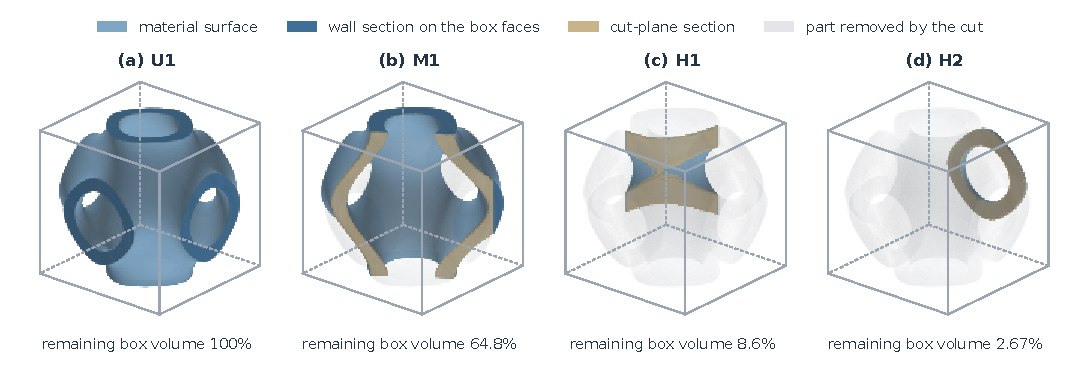
\includegraphics[width=\textwidth,height=0.8\textheight,keepaspectratio]{../figures/F08_geometry.pdf}
\caption{\textbf{代表性验证几何。} (a) 未切割 U1、(b) 中度切割 M1 以及 (c,d) 重度切割 H1 和 H2 采用相同的单位盒尺度与观察方向。蓝色表示材料表面，沙色表示切割平面上的截面。百分比表示切割后剩余的盒体积相对于单位盒的比例，未与薄壁材料求交。表面由式 (1) 在每轴 129 个位置的网格上重构，仅用于可视化。}\label{fig:1}
\end{figure}

\subsection{保留自由度与平衡延拓}

对每个胞，保留自由度汇集于集合 \(P\)，包括激活的盒面位移自由度，以及所有带有正面积切割表面片的激活单元的全部位移自由度。这些单元，即被切割平面穿过的激活单元层，构成切割带：尽管其部分节点远离切割平面，它们的基函数仍对该平面上的位移和虚功有贡献。这一完整的保留空间同时包含胞间自由度与外边界自由度，在预测与装配中始终使用。

记 \(I\) 为其余的内部自由度，\(p=|P|\)，\(i=|I|\)，\(n_a=p+i\)。选择算子 \(J_P\) 和 \(J_I\) 从激活位移向量中提取这两个集合，\(q=J_Pu\) 为保留位移。边界载荷通过 \(q\) 作用；内部体载荷为零。按所示的 \((P,I)\) 排序，静力凝聚给出

\[
\begin{aligned}
&K=\begin{bmatrix}K_{PP}&K_{PI}\\K_{IP}&A\end{bmatrix},\qquad
A=K_{II},\qquad
E=\begin{bmatrix}I_p\\-A^{-1}K_{IP}\end{bmatrix},\\
&S=K_{PP}-K_{PI}A^{-1}K_{IP}=E^TKE.
\end{aligned}
\tag{2}
\]

我们假设 \(K\succeq0\) 且 \(A\succ0\)，因此给定 \(q\) 即消除了所有内部零能运动。平衡位移延拓 \(u=Eq\) 在 \(J_Pu=q\) 上唯一地使离散能量最小，\(Sq\) 为其功共轭的保留力。对于连通的自由子结构，我们进一步假设 \(K\) 恰有六个刚体模态，即 \(R\in\mathbb R^{n_a\times6}\) 的各列，且其限制 \(R_P=J_PR\) 的秩为六。该假设依赖于稳定化离散模型的连通性，而这一连通性是有保证的：几何生成器仅接受其激活单元构成单一面连通集的胞；仅通过部分填充单元相连的材料借助共享基函数和 ghost 罚项相耦合（附录 A.1）。

\subsection{装配与响应度量}

对子结构 \(m\)，布尔装配映射 \(B_m\) 从自由的全局保留位移 \(U\) 中提取 \(q_m=B_mU\)。由背景网格位置识别的重合盒面自由度是共享的；盒面以外的保留切割带自由度仍局限于其所属子结构。由于共享面上的厚度场仅取决于该面的四个角点值，且 \(\phi\) 是周期的，两个相邻胞的材料片在每个未被切割穿过的面上重合；当切割仅从一侧移除材料时，不匹配的面自由度仍属于承载它们的胞。固定齐次支撑并入 \(B_m\)。参考装配系统与近似装配系统使用相同的映射 \(B_m\)，分别为

\[
\mathbb K=\sum_mB_m^TS_mB_m,\qquad
\widehat{\mathbb K}=\sum_mB_m^T\widehat S_mB_m,
\qquad
\mathbb K U=f_g,\quad\widehat{\mathbb K}\widehat U=f_g.
\tag{3}
\]

其中 \(\widehat S_m\) 为第 4 节的近似凝聚刚度，\(f_g\) 为作用于自由保留自由度上的给定力。由于各内部集互不相交，局部凝聚与装配可交换次序，并假设带支撑的参考矩阵 \(\mathbb K\) 正定。

柔度为 \(C=f_g^TU\)，相应有 \(\widehat C=f_g^T\widehat U\) 及相对误差 \(e_C=|\widehat C/C-1|\)。凝聚刚度的局部精度由第 3.1 节的相对方向能量误差度量。厚度灵敏度采用第 3.3 节的八分量向量，其相对欧几里得误差为 \(e_s=\|\widetilde{\boldsymbol s}-\boldsymbol s\|_2/\|\boldsymbol s\|_2\)。

第 1 节所述的要求中，有两项现在可以精确表述。\(\widehat S_m\) 必须对称半正定，且其零空间仅由保留刚体模态构成，从而使式 (3) 中带支撑的 \(\widehat{\mathbb K}\) 正定；并且其误差必须能够追溯到 \(e_C\) 和 \(e_s\)，而二者对该误差的加权方式不同。第 3 节推导任意容许延拓在这两方面能给出什么；第 4 节构造一个满足全部四项要求的凝聚刚度。

\section{近似延拓在分析与设计中的误差}

在保留自由度固定的情况下，局部近似体现在内部场上。对任意容许线性延拓（无论是否学习得到），我们将其对平衡的偏离与凝聚刚度联系起来，并考察装配与厚度求导如何对其加权；这些关系针对单个子结构陈述，并适用于装配中的每个胞。附录 B.1 汇集了相关假设。Ritz 恒等式 (4)、残差形式 (5)、式 (6) 背后的能量正交性、式 (8) 所依据的残差校正泛函以及自伴柔度灵敏度均为经典结果 \href{https://doi.org/10.1002/nme.339}{Fraeijs de Veubeke (1965)}, \href{https://doi.org/10.1007/b137868}{Toselli \& Widlund (2005)}, \href{https://doi.org/10.1017/S0962492901000010}{Becker \& Rannacher (2001)}, \href{https://doi.org/10.1007/978-94-011-2550-5}{Haftka \& Gürdal (1992)}, \href{https://doi.org/10.1007/978-3-662-05086-6}{Bendsøe \& Sigmund (2004)}；而式 (7) 与附录 C.1 中按份额加权的界、灵敏度关系 (9)--(10) 及其界（附录 H.1 和 H.2），以及附录 B.3 中的恒等式 \(\varepsilon=\delta^2\kappa\)（应用于第 5.4 节），则是本文针对近似延拓推导的。

\subsection{变分能量误差}

对于给定的对称刚度 \(K\succeq0\)，在 \(A=K_{II}\succ0\) 且内部体载荷为零时，\(Eq\) 在给定 \(q\) 下使能量最小。任意容许线性延拓 \(F\)（满足 \(J_PF=J_PE=I_p\)）与之仅在内部自由度上不同。记 \(H=J_I(F-E)\)，内部平衡 \(J_IKE=0\) 消去了 \(F\) 的凝聚刚度 \(\widehat S=F^TKF\) 中的交叉项，从而给出离散 Ritz 恒等式

\[
\boxed{\widehat S-S=H^TAH\succeq0.}
\tag{4}
\]

因此，近似延拓所增加的刚度与其内部误差的能量成正比；不存在一阶项是参考场平衡的结果。对 \(u=Eq\)、\(\widehat u=Fq\) 和 \(d_I=Hq\)，内部残差 \(r_I=(K\widehat u)_I\) 满足 \(r_I=Ad_I\)。相对方向能量误差 \(\varepsilon(q)=q^T(\widehat S-S)q/(q^TSq)\) 度量凝聚应变能超出精确应变能的部分，由式 (4) 知其非负，因而可写为

\[
\varepsilon(q)=\frac{d_I^TAd_I}{q^TSq}
=\frac{r_I^TA^{-1}r_I}{q^TSq}.
\tag{5}
\]

内部残差无需参考延拓即可获得，其 \(A^{-1}\) 范数的平方（每个方向需一次内部求解）即为刚度误差度量。附录 B 给出全方向能量误差 \(\varepsilon_*\)（式 (B.4)）。有限方向集上的最大误差给出其下界；上界只能由方向集的覆盖性得到（附录 G.4）。

\subsection{装配柔度与能量份额}

考虑式 (3) 中两个带支撑系统的精确平衡解，二者具有相同的局部矩阵、装配映射和齐次支撑，以及相同的非零保留载荷。记 \(u_m=E_mB_mU\)、\(\widehat u_m=F_mB_m\widehat U\) 以及 \(a(v,v)=\sum_m v_m^TK_mv_m\)，由全局平衡与局部能量正交性可得（附录 C）

\[
\boxed{C-\widehat C
=a(\widehat u-u,\widehat u-u)
=\|\widehat U-U\|_{\mathbb K}^{2}
+\sum_m\|H_mB_m\widehat U\|_{A_m}^{2}.}
\tag{6}
\]

因此，柔度的低估量等于重构误差的总能量，它由两部分正交贡献组成：一部分来自保留解的变化，另一部分来自该解处内部对平衡的偏离。

局部近似的影响取决于该子结构在所施载荷下承载多少能量。在精确装配迹 \(q_m=B_mU\) 处，定义能量份额 \(w_m=q_m^TS_mq_m/C\) 以及 \(\beta=\sum_mw_m\varepsilon_m(q_m)\)，并规定零能刚体响应的贡献为零。能量份额 \(w_m\) 之和为一，且

\[
0\le\frac{C-\widehat C}{C}\le\frac{\beta}{1+\beta}\le\beta.
\tag{7}
\]

因此，即使某子结构的局部场仍不准确，较小的能量份额也能削弱其对柔度的影响（附录 C.1）。

能量关系 (6) 还将算子误差与不完全装配求解的误差分离开来。对近似解 \(\bar U\)，利用所述变分算子和恢复场 \(\bar u_m=F_mB_m\bar U\)，定义重新计算的残差 \(\rho=f_g-\widehat{\mathbb K}\bar U\)。于是

\[
C-f_g^T\bar U=a(\bar u-u,\bar u-u)+\bar U^T\rho.
\tag{8}
\]

带符号的残差功 \(\bar U^T\rho\) 决定了不完全解如何影响柔度比较。附录 C.2 给出残差校正泛函，以及当数值作用与能量算子不一致时所需的附加一致性项。

\subsection{场基灵敏度与完整设计导数}

在可微的设计区间上，若激活自由度与保留自由度、装配映射、齐次支撑均固定且载荷与设计无关，则精确柔度灵敏度为 \(s_c=-u^TK_{,c}u\)，其中 \(K_{,c}=\partial K/\partial\tau_c\)；对受影响的子结构的贡献求和。内部平衡给出 \(S_{,c}=E^TK_{,c}E\)，从而在力控柔度导数中消去了精确延拓的设计导数 \href{https://doi.org/10.1023/a:1011430410075}{Giles \& Pierce (2000)}, \href{https://doi.org/10.1007/978-94-011-2550-5}{Haftka \& Gürdal (1992)}。

场基灵敏度估计 \(\widetilde s_c=-\widehat u^TK_{,c}\widehat u\) 对重构场使用相同的刚度导数。在八个角点上，它们分别构成厚度灵敏度向量 \(\boldsymbol s=(s_c)_{c=1}^8\) 和 \(\widetilde{\boldsymbol s}=(\widetilde s_c)_{c=1}^8\)。在相同的保留位移下，

\[
\widetilde s_c-s_c=-2d^TK_{,c}u-d^TK_{,c}d,
\qquad u=Eq,\quad d=Fq-Eq.
\tag{9}
\]

内部平衡使 \((Ku)_I=0\)，但一般有 \((K_{,c}u)_I\ne0\)，因此线性交叉项依然存在，能量误差的减小未必带来灵敏度误差的单调减小。由于三线性形函数非负，增厚某一角点会使材料域单调扩大；在基函数、材料与 ghost 贡献保持固定时，精确刚度导数因而是半正定的，即 \(K_{,c}\succeq0\)（式 (H.6)）。于是式 (9) 的二次项非正，但交叉项可正可负（附录 H.2）。数值导数仅在其求积保持这种嵌套关系时才继承 \(K_{,c}\succeq0\)（附录 H.2）。

代理柔度的导数还包含延拓对设计的依赖。对于仅影响一个子结构的参数，在固定保留自由度下求导得

\[
\widehat C_{,c}
=-\widehat u^TK_{,c}\widehat u
 -2\widehat q^TF_{,c}^TK\widehat u
=\widetilde s_c-2(F_{I,c}\widehat q)^Tr_I,
\qquad\widehat u=F\widehat q.
\tag{10}
\]

其中 \(\widehat q\) 为用 \(\widehat S\) 求得的装配保留解，\(r_I=(KF\widehat q)_I\)，\(F_{I,c}=J_I\partial F/\partial\tau_c\)；对受影响子结构的贡献求和。第二项将延拓的设计依赖性与其内部不平衡相耦合，对平衡延拓而言该项为零。本文报告的所有灵敏度均为场基估计 \(\widetilde s_c\)，即第一项：它们估计的是精确灵敏度，而非代理柔度的导数。仅凭能量精度并不能控制完整导数（附录 H.2，第 6.2 节）。附录 H 给出数值刚度导数的具体形式。

上述导数在附录 B.1 所列的离散选择（激活单元、ghost 面、保留自由度、网络的二值节点指示量以及校正的离散选择）保持固定的区间上成立；其中任一项发生变化即为离散模型切换。跨越切换时，离散参考柔度本身可能发生跳跃，正如在同一背景网格上进行精确凝聚时那样；由于在每个设计处均有 \(0\le C-\widehat C\le\beta C\)（式 (7)），代理柔度额外引入的任何跳跃均以其自身误差水平为界（补充说明 S4.3）。

对于第 4 节的构造，这些关系将第 1 节和第 2.3 节的要求转化为对延拓的三个条件：其内部误差能量在装配解所选取的方向上必须很小，式 (5) 通过内部残差表达了这一点；部署时施加的校正不得增大该能量，从而由式 (4) 使校正后的凝聚刚度介于未校正凝聚刚度与精确 Schur 补之间（第 4.3 节）；并且，由于能量误差不能控制式 (9) 的灵敏度误差，灵敏度必须独立于柔度单独验证（第 5.6 节和第 5.10 节）。

\section{带平衡校正的神经初始化静力凝聚}

该构造包含三个部分。学习延拓提供试探内部场（第 4.4 节）；以完整延拓的转置作用的能量形式提供力学结构（第 4.1 节）；校正 \(\mathcal W\) 提供可改进性（第 4.2 节和第 4.3 节）。图 2 展示了这三部分如何共同定义凝聚作用以及装配后恢复的位移。我们首先介绍该力学对象，然后介绍改进它的校正，最后介绍对其进行初始化的网络。

\begin{figure}[!htbp]
\centering
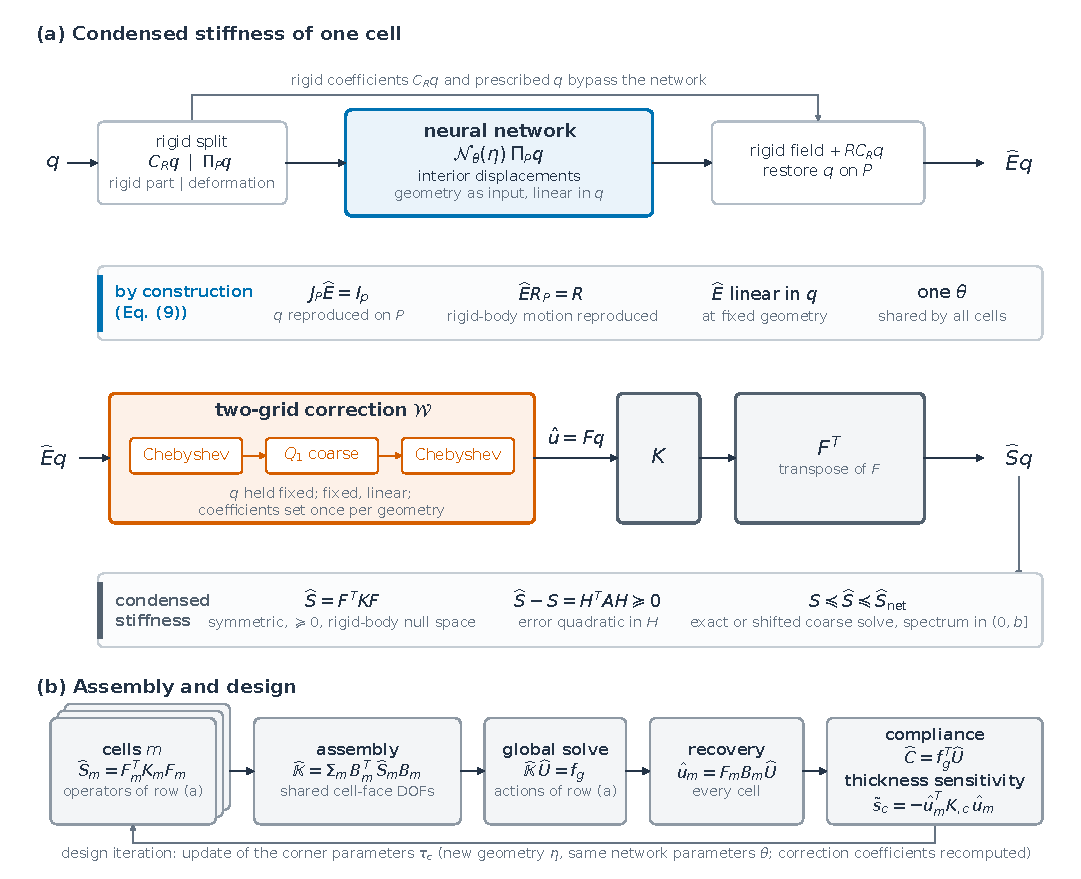
\includegraphics[width=\textwidth,height=0.8\textheight,keepaspectratio]{../figures/F01_method_overview.pdf}
\caption{\textbf{学习位移延拓、平衡校正与变分装配。} (a) 在由网络延拓变形之前，先从保留位移中分离出刚体运动。随后重构刚体场并恢复给定的保留值；校正 \(\mathcal W\) 接着在固定保留位移下减小内部不平衡，再施加局部刚度和完整延拓的转置 \(F^T\)，即得到功共轭的保留力。(a) 中的排序假设粗网格校正精确，且光滑区间的上端界住谱；它对能量误差排序，而非对灵敏度误差排序。(b) 各胞算子在共享盒面自由度上装配，并求解装配系统；装配解为局部场恢复、柔度和场基厚度灵敏度提供输入。一次设计迭代更新角点厚度参数，从而重新生成每个胞的几何；网络参数保持不变，而 \(\mathcal W\) 的系数则重新计算。}\label{fig:2}
\end{figure}

\subsection{变分凝聚刚度}

设 \(\widehat E\) 为容许延拓，\(J_P\widehat E=I_p\)，且能再现刚体运动，即对第 2.2 节的刚体模态 \(R\) 有 \(\widehat ER_P=R\)；第 4.4 节用几何条件化网络构造该延拓（式 (17)）。延拓通过其所产生场在原始刚度下的能量而成为力学算子。设内部校正 \(\mathcal W\) 为在固定保留位移下的一次两层网格循环（Chebyshev 光滑、粗网格 Galerkin 校正与光滑；第 4.2 节和第 4.3 节）；它就是方法名称中的平衡校正。该校正是线性的且保持保留值不变，恒等映射对应于不校正。对每一几何，校正方案及其系数的确定与保留位移无关。最终延拓及其凝聚刚度为

\[
F=\mathcal W\widehat E,\qquad
\widehat S=F^TKF,\qquad
\widehat{\mathcal U}(q)=\tfrac12q^T\widehat S q,\qquad
\widehat f_P=\widehat S q.
\tag{11}
\]

对虚保留位移 \(\delta q\)，相应的完整虚场为 \(F\delta q\)，且 \(\delta\widehat{\mathcal U}=(F\delta q)^TKFq=\delta q^TF^TKFq\)。因此，施加凝聚算子需要在刚度作用之后再施加完整延拓（包括刚体重构、保留值恢复与校正）的转置 \(F^T\)。记 \(F_I=J_IF\)，凝聚作用具有分块形式

\[
\widehat S q=(KFq)_P+F_I^T(KFq)_I.
\tag{12}
\]

第二项将内部残差的功传递到保留自由度上。对平衡场该项为零；否则，必须有该项，返回的力才是所述能量的导数。对称性与半正定性源于 \(K=K^T\succeq0\)，而不要求学习得到的收集、散布或网格传递映射具有对称性。在第 2.2 节关于刚体核的假设以及 \(FR_P=R\) 下，\(\widehat S\) 的零模态仅为保留刚体模态（附录 B）；附录 E 推导转置 \(F^T\)，附录 B.2 说明它为何使算子误差成为二次的。由式 (4)，\(\widehat S-S=H^TAH\)，其中 \(H=J_I(F-E)\)：算子误差即 \(F\) 的内部误差的能量，第 4.2 节和第 4.3 节将其减小。完成装配求解后，\(F_mB_m\widehat U\) 提供用于响应与灵敏度评估的局部重构位移。

\subsection{误差谱与 Chebyshev 光滑}

式 (5) 和式 (6) 表明，可在保留运动固定的条件下减小学习场的内部不平衡；多项式光滑 \href{https://doi.org/10.1016/s0021-9991(03)00194-3}{Adams et al. (2003)} 与粗能量极小化分别处理其中的不同分量。

令 \(D=\operatorname{diag}(A)\)，并将广义特征向量 \(Av_j=\lambda_jDv_j\) 按特征值递增排序，且 \(v_j^TDv_k=\delta_{jk}\)。对于 \(c_j=v_j^TDd_I\)，有

\[
d_I^TAd_I=\sum_j\lambda_jc_j^2,\qquad
\chi_\ell(q)=\frac{\sum_{j=1}^{\ell}\lambda_jc_j^2}{d_I^TAd_I}.
\tag{13}
\]

比例 \(\chi_\ell\) 刻画误差能量在前 \(\ell\) 个 Jacobi 缩放内部模态中的分布（精确场的相应比例使用 \(u_I^TAu_I\)）。

学习场是 \(Au_I=-K_{IP}q\) 的初始近似，在 \(q\) 固定的条件下通过 Jacobi 预条件 Chebyshev 半迭代 \href{https://doi.org/10.1007/BF01386013}{Golub \& Varga (1961)} 加以改进；规定的迭代次数和依赖于几何的系数保证校正后的延拓保持线性。以这种方式将学习得到的初值与光滑相结合，与光滑聚集延拓 \href{https://doi.org/10.1007/BF02238511}{Vaněk et al. (1996)} 相呼应，也与混合求解器的思路一致，即由松弛消除学习预测所遗留的高频误差 \href{https://doi.org/10.1038/s42256-024-00910-x}{Zhang, E. et al. (2024)}。

\(k\) 次误差多项式将 \(d_I\) 映射为 \(\Phi_kd_I\)，其中 \(\Phi_k=p_k(D^{-1}A)\)，即将式 (13) 中的每个系数乘以 \(p_k(\lambda_j)\)。Chebyshev 多项式以 \([a,b]\)（\(0<a<b\)）为目标区间；若 \(D^{-1/2}AD^{-1/2}\) 的实际正谱位于 \((0,b]\) 内，则该多项式在 \(A\) 能量范数下是非扩张的。低于 \(a\) 的模态可能衰减缓慢，这正是引入互补的粗网格校正的动因。校正序列取 \(a=b/30\)，其中 \(b\) 由幂迭代估计值增大 5\% 得到；第 5.2 节报告了对其的验证，附录 D 给出了多项式、递推关系、区间估计子以及收缩界。

\subsection{粗网格校正}

设 \(V\in\mathbb R^{i\times n_c}\) 列满秩，\(A_c=V^TAV\)，\(b_r=V^Tr_I\)。记 \(\widehat u_I\) 为当前的近似内部场（学习场或光滑后的迭代值），\(r_I=(K\widehat u)_I\) 为其内部残差，在 \(\widehat u_I+\operatorname{range}V\) 上极小化能量，得到

\[
\widehat u_I^{\rm c}=\widehat u_I-VA_c^{-1}b_r,\qquad
d_I^{\rm c}=(I_i-VA_c^{-1}V^TA)d_I,\qquad
\|d_I\|_A^2-\|d_I^{\rm c}\|_A^2=b_r^TA_c^{-1}b_r.
\tag{14}
\]

粗网格（Galerkin）校正对粗变分施加平衡条件，最后一个等式度量了该投影所消除的能量 \href{https://doi.org/10.1137/1034116}{Xu (1992)}。主粗基记为 \(Q_1(17)\)，由 \(17^3\) 顶点网格上限制于内部自由度的三线性向量函数构成（附录 F.1）；所有粗空间都只作用于内部自由度，因此保留值保持不变。

将粗网格校正置于两个 \(k\) 步光滑阶段之间，即可把这些校正组合为一个两层网格循环，也就是第 4.1 节中的校正 \(\mathcal W\)。记 \(C_V=I_i-VA_c^{-1}V^TA\)，\(H_{\rm net}=J_I(\widehat E-E)\)，则两层网格误差算子 \(\Phi_kC_V\Phi_k\) \href{https://doi.org/10.1007/978-3-662-02427-0}{Hackbusch (1985)}, \href{https://shop.elsevier.com/books/multigrid/trottenberg/978-0-12-701070-0}{Trottenberg et al. (2001)}, \href{https://doi.org/10.1090/S0894-0347-02-00398-3}{Xu \& Zikatanov (2002)}, \href{https://doi.org/10.1002/nla.437}{Falgout et al. (2005)} 给出 \(F\) 的内部误差，并由式 (4) 给出算子误差

\[
H=\Phi_kC_V\Phi_kH_{\rm net},\qquad
\widehat S-S=H^TAH.
\tag{15}
\]

若粗网格校正是精确的且 \(\|\Phi_k\|_A\le1\)，则 \(S\preceq\widehat S\preceq\widehat S_{\rm net}\)，其中 \(\widehat S_{\rm net}=\widehat E^TK\widehat E\) 为未校正凝聚刚度。因此，校正不会增大 \(A\) 能量范数下的误差，并且根据附录 C 的序反转关系，它使装配后的柔度向参考解靠近（附录 D.1）。该序关系是有保证的，但减小的幅度则没有保证（附录 D），第 5.5 节对其进行了测量。该序关系不能推广到式 (9) 的灵敏度误差（附录 D.1）；此外，改变光滑次数会改变多项式，因此误差的减小不一定关于 \(k\) 单调。

\subsection{几何条件化多层位移延拓}

学习目标是内部平衡映射 \(q\mapsto E_Iq=-A^{-1}K_{IP}q\)；其近似既给出位移场，又通过其能量给出完整保留空间上的凝聚算子。网络架构必须适应每个胞的材料分布与支撑情况，并在几何固定时满足叠加原理。保留集包含 2,679 至 45,900 个自由度，且随切割而变化，因此既无法为每个几何构造延拓矩阵（每个保留自由度需要一次内部求解），也无法采用对每个保留自由度各设一个输出的网络。由此得到一个非线性几何分支与一个线性多层位移分支相耦合的结构，其权重作用于模板、通道和网格层级（图 3）。

刚体运动在学习之前被分离出来。取 \(R\) 的各列为三个平移以及绕同一中心的三个转动。系数提取算子 \(C_R=(R_P^TR_P)^{-1}R_P^T\) 与投影算子 \(\Pi_P=I_p-R_PC_R\) 将输入分解为刚体系数 \(C_Rq\) 与保留变形 \(q_d=\Pi_Pq\)。网络只延拓 \(q_d\)，因此刚体重构与训练精度无关。

在几何分支中，单元矩刻画每个背景单元内的材料分布，节点特征则标识节点是否属于保留集和切割带、是否为弱支撑节点（对角刚度块低于活动节点中位数的 1\%；附录 G），以及局部刚度大小和位置。编码器生成单元与节点特征向量，二者经过两轮信息交换；随后由系数头（小型输出网络）为规定的单元与 ghost 面关联、潜在网格之间的传递以及粗网格卷积分配权重。对于同一几何，这些系数对所有位移方向保持不变。

位移分支将 \(q_d\) 的三个分量提升为保留节点上的 32 个通道，内部特征置零，由此定义 \(X^0(q)\)。局部相互作用通过单元与 ghost 面邻域传播这些值：每个相互作用将 27 槽模板上的特征汇聚到四个加权头中，在每个头内混合通道，并将结果散布回相关节点。记作用于节点行的内部掩码和保留掩码为 \(M_I,M_P\)，一次相互作用按下式更新潜在场：

\[
X^{\ell+1}=M_I\left[X^\ell+
 \sum_h\mathcal S_{\ell h}(\eta)
   \big(\mathcal G_{\ell h}(\eta)X^\ell W_{\ell h}\big)\right]
 +M_PX^0(q).
\tag{16}
\]

其中 \(\mathcal G_{\ell h}\) 和 \(\mathcal S_{\ell h}\) 为几何加权的汇聚与散布映射，\(W_{\ell h}\) 混合通道，最后一项恢复保留特征。一个经过每轴 65、33、17 和 9 个位置网格的 U 形潜在层级提供更长程的信息传递；在其前后各有若干对局部相互作用，另有若干对作用于含弱支撑节点的模板，共同构成该分支，最后由一个线性映射重构节点位移（图 3b,c）。权重作用于模板、通道和网格层级，而非单个自由度，因此同一个网络（约 \(6\times10^5\) 个参数；表 ST15）适用于所有保留集。附录 G 给出了完整的运算顺序与系数定义。

所有位移运算都是线性的，而非线性编码器只作用于几何，因此以 \(\theta\) 为网络参数的原始映射 \(\mathcal N_\theta(\eta)\) 在 \(\eta\) 固定时满足叠加原理。加回刚体场并恢复原始保留值，得到

\[
\widehat E q=J_P^Tq+
J_I^TJ_I\left[RC_Rq+\mathcal N_\theta(\eta)\Pi_Pq\right].
\tag{17}
\]

因此 \(J_P\widehat E=I_p\) 且 \(\widehat ER_P=R\)：容许性与刚体再现性由构造保证。

\begin{figure}[!htbp]
\centering
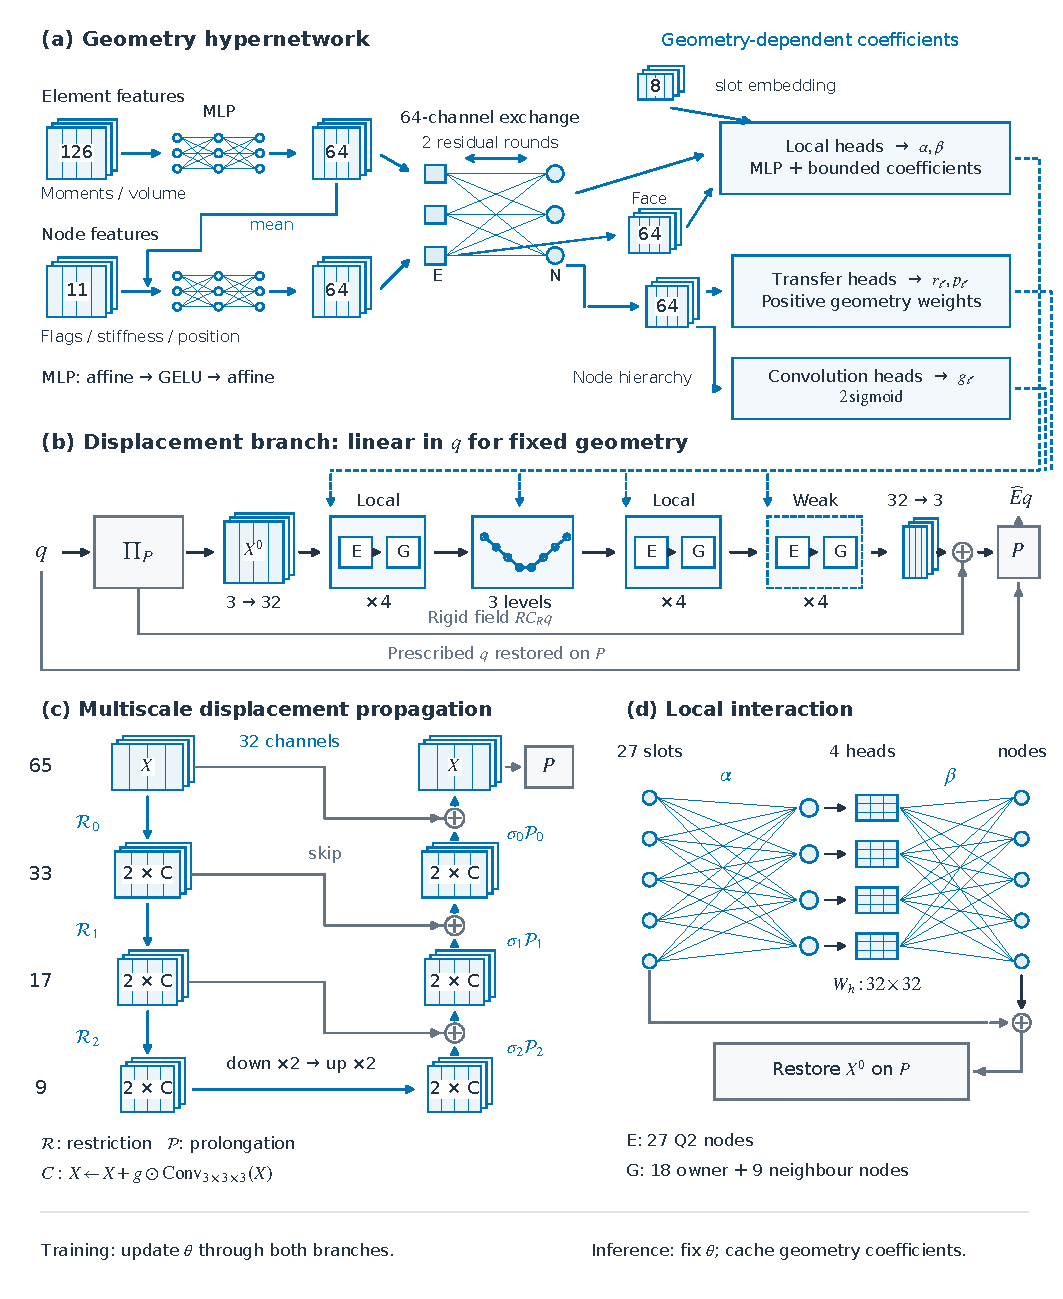
\includegraphics[width=\textwidth,height=0.8\textheight,keepaspectratio]{../figures/F11_network_architecture.pdf}
\caption{\textbf{几何条件化神经位移架构。} (a) 单元与节点编码器生成 64 通道几何特征向量，随后进行两轮残差交换；系数头为局部相互作用、网格传递和卷积提供条件。(b) 位移分支将非刚体保留输入依次经过四对局部相互作用、多层模块、另外四对局部相互作用以及四对作用于弱支撑模板的相互作用进行传播；线性映射连接三个位移分量与 32 个潜在通道，确定性旁路重构刚体运动并恢复保留值。(c) 限制与延拓连接每轴具有 65、33、17 和 9 个背景位置的网格；每个粗层级在每次经过时包含两个残差卷积。(d) 局部相互作用采用几何加权汇聚、四个通道混合头和散布，随后进行残差相加与保留值恢复。E 和 G 分别表示单元相互作用与 ghost 面相互作用。蓝色虚线箭头传递依赖于几何的系数；实线箭头传递特征或位移状态。对于固定几何，完整的位移路径是线性的。}\label{fig:3}
\end{figure}

\subsection{训练方向与目标函数}

训练通过保留位移方向来考察延拓：规定的多项式位移和多尺度位移提供广泛的空间内容，而在平衡节点载荷、一致面力、弹簧支撑和邻胞作用下的响应则提供力学生成的方向。去除刚体分量后，利用参考解将每个方向归一化为 \(q_j^TSq_j=1\)。对于一批 \(B\) 个方向，目标函数为

\[
\mathcal L(\theta)=\frac1B\sum_{j=1}^{B}\log(q_j^T\widehat S q_j)
 +w_s\frac1{|\mathcal J_s|}\sum_{j\in\mathcal J_s}
 \frac{\|\widetilde{\boldsymbol s}_j-\boldsymbol s_j\|_2^2}{\|\boldsymbol s_j\|_2^2}.
\tag{18}
\]

能量项是预测能量与参考能量之比的对数平均值。对于容许延拓，第 3.1 节的变分恒等式使其最小值对应于每个采样方向上的平衡场，即 Ritz 原理。灵敏度项在带有参考灵敏度标签的方向集 \(\mathcal J_s\) 上比较场基厚度灵敏度（八分量向量）；文中报告的配置取 \(w_s=1\)。关于 \(\theta\) 的梯度经由重构场传递至几何编码器、系数头和线性位移映射。训练过程中会加入能量比较大的方向（通过在刚体补空间上进行块搜索得到），几何增广则利用立方体的 48 种对称性（附录 G）。表 2 列出了各变体，表 ST01 记录了训练与模型选择的设置。

NICE 针对实际部署的算子进行训练：式 (18) 在校正后的延拓 \(F=\mathcal W\widehat E\) 上计算，其中在第 4.3 节的 \(Q_1(17)\) 粗网格校正前后各进行八步 Chebyshev 光滑（记为 8 / \(Q_1(17)\) / 8；表 1）。由于对给定几何而言 \(\mathcal W\) 是线性且固定的，梯度可穿过光滑递推和粗网格校正传递到网络参数，这与求解器在环训练 \href{https://proceedings.neurips.cc/paper/2020/hash/43e4e6a6f341e00671e123714de019a8-Abstract.html}{Um et al. (2020)} 类似。光滑区间和粗分解仅依赖于 \(K\)，并针对每个几何重新计算，因此不引入任何可训练参数。

\subsection{凝聚算子的作用}

依赖于几何的量对每个几何只准备一次，并在不同保留输入之间复用：单元矩、网络的几何编码、系数与映射、光滑区间以及粗分解（表 ST13 给出了其计算代价）。此后，\(\widehat S\) 的每次作用需要一次网络前向传递、\(2k\) 步光滑、一次粗求解以及相应的转置序列（附录 E--F）。\(\widehat E\) 和 \(\widehat S\) 均不显式形成：每个胞只存储其依赖于几何的系数和粗分解；而对于保留规模为中位数（\(2.4\times10^4\) 个自由度）的胞，稠密的 \(\widehat S\) 在双精度下将占用 4.3 GiB。

\textbf{算法 1. 校正后凝聚刚度的作用。}

\begin{enumerate}
\def\labelenumi{\arabic{enumi}.}
\tightlist
\item
  用 \(\widehat E\) 延拓 \(q\)，并在保留值固定的条件下依次施加规定的前光滑、粗网格校正和后光滑，得到 \(\widehat u=Fq\)。
\item
  计算 \(y=K\widehat u\) 并返回 \(F^Ty\)：按相反顺序施加完整校正的转置，再施加学习延拓的转置。
\item
  通过式 (3) 装配这些作用；全局求解之后，恢复 \(F_mB_m\widehat U\) 以用于场和灵敏度的计算。
\end{enumerate}

\section{数值算例}

各算例追踪学习延拓的误差：从单个胞出发，经过其校正，到装配后的响应，再到设计。第 5.1 节和第 5.2 节定义几何、变体和载荷，并验证离散参考解与所部署的算子。第 5.3--5.5 节考察单个胞的算子：其对几何和载荷的依赖性、误差的组成，以及在网络参数固定时校正所消除的部分。第 5.6--5.7 节考察装配后的响应：两胞配置中的柔度与局部灵敏度、能量份额，以及对保留表示的消融。第 5.8 节和第 5.9 节装配所有胞均为学习子结构的格栅，并将其计算代价与整体格栅直接求解和常规精确凝聚进行比较；第 5.10 节利用该算子优化厚度场，并以精确凝聚对所得设计进行验证。

\subsection{几何、变体与载荷条件}

80 个验证几何包括 20 个未切割胞、20 个轻度切割胞、20 个中度切割胞和 20 个重度切割胞，其厚度场为均匀、仿射或混合三线性分布，角点参数介于 0.1762 与 0.6983 之间（表 ST02）。每个胞至多带有一个平面切割，其法向为 \((\cos\vartheta,\sin\vartheta,0)\)，\(0<\vartheta<\pi/4\)；重度切割保留的体积不足胞盒体积的三分之一，中度切割介于三分之一与三分之二之间，轻度切割则超过三分之二。U、L、M 和 H 分别标识用于详细比较的未切割、轻度切割、中度切割和重度切割胞（U1、U2、L1、M1、M2 以及 H1--H3；补充材料 R1）。表 1 列出了离散化与校正设置。

每个验证几何均用表 ST03 中九个验证类别（定义见附录 G.2）的保留位移方向进行考察：施加的多项式位移和多尺度位移、作用于所有面或单个面的平衡节点力与一致面力、弹簧支撑下的响应，以及由邻胞诱导的迹。一致面力（每个几何 64 个方向）代表表面载荷和邻胞面力，是主要的载荷类别；等值节点力还会加载弱支撑节点，用作对稳定化问题的压力测试：在表 ST04 的五个胞中，一致面力作用下 ghost 罚项平均承担不到精确场能量的 0.05\%，而在等值节点力作用下则承担 49--81\%。

{\small
\begin{longtable}[]{@{}
  >{\raggedright\arraybackslash}p{(\linewidth - 2\tabcolsep) * \real{0.5000}}
  >{\raggedright\arraybackslash}p{(\linewidth - 2\tabcolsep) * \real{0.5000}}@{}}
\caption{离散化与校正设置}\tabularnewline
\toprule\noalign{}
\begin{minipage}[b]{\linewidth}\raggedright
量
\end{minipage} & \begin{minipage}[b]{\linewidth}\raggedright
设置
\end{minipage} \\
\midrule\noalign{}
\endfirsthead
\toprule\noalign{}
\begin{minipage}[b]{\linewidth}\raggedright
量
\end{minipage} & \begin{minipage}[b]{\linewidth}\raggedright
设置
\end{minipage} \\
\midrule\noalign{}
\endhead
\bottomrule\noalign{}
\endlastfoot
参考几何 & 单位盒；带三线性角点参数的 Schwarz-P 型隐式带，可选一个平面切割 \\
位移近似 & 笛卡尔背景网格上的连续张量积 \(Q_2\) 实体单元 \\
背景分辨率（验证几何） & 每轴 \(n=32\) 个单元；每轴 \(65\) 个 Q2 节点 \\
各向同性材料（验证几何） & 归一化杨氏模量 \(E_Y=1\)，泊松比 \(\nu=0.3\) \\
ghost 罚项系数（验证几何） & \(\gamma=10^{-4}\) \\
保留空间 & 活动盒面自由度，以及所有含正面积切割面片的活动单元的全部自由度 \\
标准体积积分 & \(4^3\) 个初始子胞；对部分子胞进行一次局部加密；裁剪后的 Kuhn 四面体，求积规则参数为 4 \\
光滑区间 & \([b/30,b]\)，其中 \(b\) 取 \(\lambda_{\max}(D^{-1}A)\) 的 40 步幂迭代估计值的 1.05 倍（第 4.2 节） \\
主内部粗空间 & \(17^3\) 顶点网格上的三线性向量函数，限制于内部自由度 \\
厚度差分步长 & \(h_c=10^{-5}\tau_c\)，活动自由度和 ghost 贡献保持固定 \\
NICE 的校正 & 8 步 Chebyshev 光滑、\(Q_1(17)\) 粗网格 Galerkin 校正、8 步 Chebyshev 光滑；训练与评估采用相同序列 \\
算术精度 & 网络采用单精度；刚度作用与能量采用双精度；校正在精度研究中采用双精度，在表 5 的计时流程和第 5.10 节的优化中采用单精度（附录 F.2） \\
\end{longtable}}

网格、材料和稳定化条目适用于全部 80 个验证几何；长度均相对于单位盒，模量经过归一化。其他校正序列的粗空间维数和光滑步数在相应比较中给出。

共比较四种变体（表 2）。基础网络在无校正条件下训练。另有三个网络在其基础上继续训练 15,000 步：在训练回路中包含第 4.2 节和第 4.3 节的完整校正 \(\mathcal W\)（NICE，第 4.5 节）；在每个训练步中采用八步光滑而不进行粗网格校正（平滑训练）；或不加校正（未校正，正文中称为未校正延续）。

{\small
\begin{longtable}[]{@{}
  >{\raggedright\arraybackslash}p{(\linewidth - 8\tabcolsep) * \real{0.1875}}
  >{\raggedright\arraybackslash}p{(\linewidth - 8\tabcolsep) * \real{0.1875}}
  >{\raggedleft\arraybackslash}p{(\linewidth - 8\tabcolsep) * \real{0.2500}}
  >{\raggedright\arraybackslash}p{(\linewidth - 8\tabcolsep) * \real{0.1875}}
  >{\raggedright\arraybackslash}p{(\linewidth - 8\tabcolsep) * \real{0.1875}}@{}}
\caption{数值算例中比较的变体}\tabularnewline
\toprule\noalign{}
\begin{minipage}[b]{\linewidth}\raggedright
变体
\end{minipage} & \begin{minipage}[b]{\linewidth}\raggedright
网络参数
\end{minipage} & \begin{minipage}[b]{\linewidth}\raggedleft
训练集（几何数）
\end{minipage} & \begin{minipage}[b]{\linewidth}\raggedright
训练中的校正
\end{minipage} & \begin{minipage}[b]{\linewidth}\raggedright
评估时的校正
\end{minipage} \\
\midrule\noalign{}
\endfirsthead
\toprule\noalign{}
\begin{minipage}[b]{\linewidth}\raggedright
变体
\end{minipage} & \begin{minipage}[b]{\linewidth}\raggedright
网络参数
\end{minipage} & \begin{minipage}[b]{\linewidth}\raggedleft
训练集（几何数）
\end{minipage} & \begin{minipage}[b]{\linewidth}\raggedright
训练中的校正
\end{minipage} & \begin{minipage}[b]{\linewidth}\raggedright
评估时的校正
\end{minipage} \\
\midrule\noalign{}
\endhead
\bottomrule\noalign{}
\endlastfoot
\textbf{NICE} & 基础网络继续训练 15,000 步 & 591 & 8 / \(Q_1(17)\) / 8 & 8 / \(Q_1(17)\) / 8 \\
平滑训练 & 基础网络继续训练 15,000 步 & 591 & 8 步光滑 & 8 步光滑 \\
未校正 & 基础网络继续训练 15,000 步 & 591 & 无 & 无 \\
基础网络 & 训练 40,000 步，于第 30,000 步选定 & 305 & 无 & 无 \\
\end{longtable}}

此外还评估了在部署时施加校正 \(\mathcal W\) 而不重新训练的基础网络，记为``基础网络（加校正）''（第 5.3、5.5 和 5.6 节）。

所有变体共享第 4 节的架构（约 \(6\times10^5\) 个可训练参数；表 ST15）。三个延续训练均取自同一个包含 591 个几何的集合，其中包含基础网络 305 个训练几何中的 304 个，并且以相同顺序遍历相同的几何（表 ST01）。在一块 RTX 5090 GPU 上，基础网络的训练耗时 4.6 h，NICE 的延续训练耗时 3.5 h；为 691 个训练与验证几何生成方向和精确灵敏度约耗时 42 GPU 小时；数据生成、训练与模型选择合计约耗时 60 GPU 小时（表 ST01）。

80 个验证几何中有 20 个（6 个未切割，14 个切割）用于检查点选择（表 ST01）；因此也针对选择之外的 60 个几何给出了统计结果。第 5.6 节两胞装配中的目标胞属于这 20 个选择几何；另有九个选择之外的胞在该节中进行装配，作为独立检验。总体统计先在每个几何和载荷类别内对方向能量误差取平均，再对各几何等权处理（附录 A.1），因此总体最大值即为最大的几何平均值。

\subsection{离散参考解与校正算子的验证}

\(n=32\) 参考解通过在七个胞上的加密进行了验证：U1 加密至 \(n=40\)，M1 和 M2 加密至 \(n=48\)（图 S01），H1、H2 及另外两个验证胞加密至 \(n=64\)（表 ST10；补充说明 S1）。未切割和中度切割胞的柔度变化至多 0.14\%，其厚度灵敏度变化至多 0.23\%；而对于重度切割胞，柔度变化最高约 1\%，灵敏度变化最高达 3.6\%，二者均出现在 H2 中。将 ghost 罚项系数在 \(10^{-5}\) 与 \(10^{-3}\) 之间变化以及加密体积积分，使柔度和灵敏度的变化至多为 0.12\%；有限差分刚度导数及其步长在补充说明 S1 中进行了验证（图 S01(c)）。以下所有比较均以该离散参考解为基准（第 2.1 节）。

我们在表 1 的算术设置下，针对 U2、M1、M2、H1 和 H2 每个胞的前八个一致面力验证方向，检验了部署算子。双线性形式 \(q_i^T\widehat Sq_j\) 在相对 \(9\times10^{-9}\) 的精度内对称。返回的功 \(q^T\widehat Sq\) 与恢复场能量 \(q^TF^TKFq\) 的吻合程度达 \(5\times10^{-9}\)。部署算子复现训练时场的精度为 \(1.1\times10^{-7}\)。归一化刚体模态所携带的能量至多为典型变形能量的 \(2\times10^{-11}\)。在前八个节点力方向上，非对称性、功--能量差及刚体能量比分别至多为 \(3\times10^{-8}\)、\(2\times10^{-8}\) 和 \(1\times10^{-10}\)（表 ST04）。

第 4.2 节的非扩张性要求 \(b\ge\lambda_{\max}(D^{-1}A)\)。在全部 80 个验证几何上，幂迭代端点比收敛的最大特征值高出 2.1--5.0\%（附录 D），而有保证的 Gershgorin 界则大 4.7 至 19.4 倍（中位数 18.4），会使光滑区间远高于实际谱。因此，该谱条件在这些几何上得到了数值支持；对于第 5.8--5.10 节中格栅和优化所用的胞，虽然采用相同的幂迭代估计，但未对其进行检验。对称性、半正定性以及 \(\widehat S\succeq S\) 均不依赖于该条件。

\subsection{对几何与载荷的依赖性}

NICE 的分层平均误差比未校正延续低 64 至 102 倍，尽管其误差从未切割胞到重度切割胞仍增长约七倍（图 4）。在一致面力下，NICE 在未切割、轻度切割、中度切割和重度切割分层中的平均方向能量误差分别为 0.016\%、0.079\%、0.091\% 和 0.109\%，未校正延续则分别为 1.03\%、5.33\%、7.82\% 和 11.2\%（补充表 ST03b）。在全部 80 个几何上，NICE 的平均值为 0.074\%，未校正延续为 6.33\%，基础网络为 6.89\%；三者最大的几何平均值分别为 0.65\%、42\% 和 48.6\%。逐方向来看，NICE 在 5,120 个采样一致面力方向上的误差，第 95 百分位数为 0.33\%，第 99 百分位数为 0.69\%，最大值为 1.24\%（在检查点选择之外的 60 个几何上分别为 0.35\%、0.73\% 和 1.24\%）。

在其他载荷类别下，NICE 在邻胞诱导位移下的平均值为 0.060\%（最大 0.38\%），在刚度缩放弹簧支撑下为 0.057\%（0.47\%）；对于单面节点力，其最大几何平均值为 0.72\%（表 ST03；各几何的分布见图 S02）。在节点力下，基础网络的平均值从未切割胞的 0.908\% 上升至重度切割胞的 11.3\%（最大 70.1\%），而 NICE 的分层平均值保持在 0.013\% 至 0.090\% 之间（最大 0.325\%）。在选择之外的 60 个几何上，NICE 的总体平均值基本不变（一致面力下为 0.077\%，节点力下为 0.059\%），但在一致面力下其切割分层平均值更高（中度 0.105\%，重度 0.126\%），且五个最大的几何平均值均出自这 60 个几何（补充表 ST03）。

中间变体揭示了这一改进的来源。不加校正地对基础网络进行延续训练，仅使其平均值从 6.89\% 变为 6.33\%；平滑训练达到 1.28\%（最大 7.8\%）。不经重新训练、直接对基础网络施加校正，即已得到 0.0965\%（最大 0.91\%），因此大部分改进来自校正本身；NICE 延续训练还增加了训练并扩大了训练池，使平均值进一步降低为原来的 1/1.31（基于几何的 95\% bootstrap 区间为 1.20--1.40；补充表 ST03）。

\begin{figure}[!htbp]
\centering
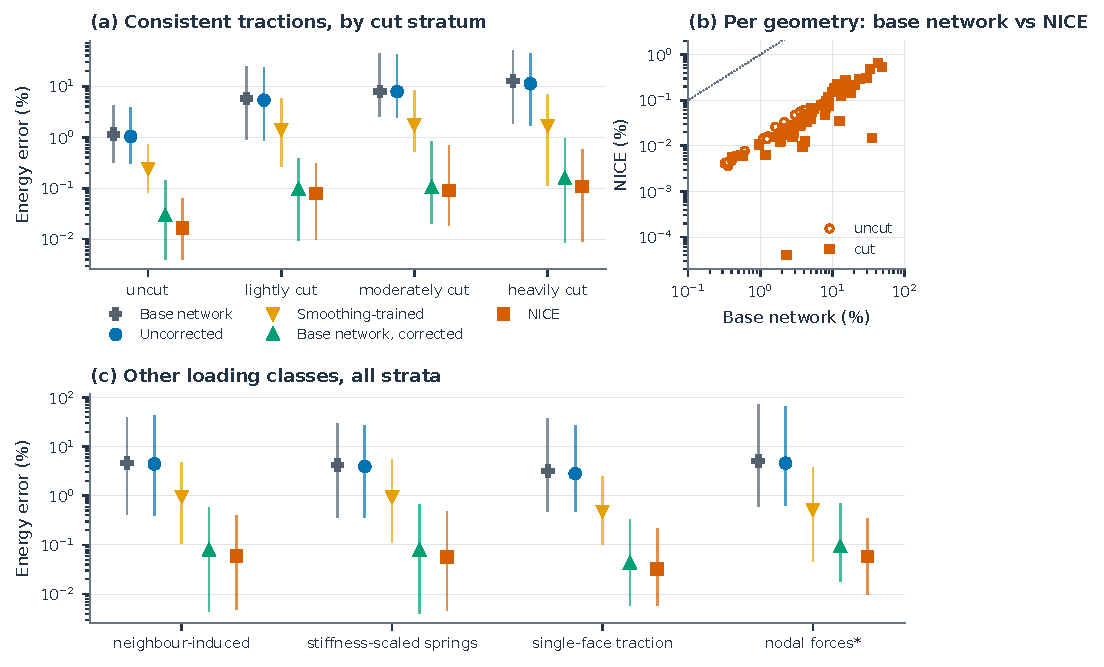
\includegraphics[width=\textwidth,height=0.8\textheight,keepaspectratio]{../figures/F02_validation.pdf}
\caption{\textbf{学习子结构在 80 个验证几何上的方向能量误差。} 每个观测值为某一几何在某一载荷类别各验证方向上的平均方向能量误差 \(q^T(\widehat S-S)q/(q^TSq)\)。(a) 一致面力，每个切割分层 20 个几何：标记表示各几何的平均值，误差棒表示从第 10 百分位数到最大值的范围。(b) 一致面力下基础网络与 NICE 的几何平均值，空心标记表示未切割几何，实心标记表示切割几何；点线表示相等。(c) 邻胞诱导保留位移、刚度缩放弹簧支撑、单面一致面力与等值节点力（前两类为 75 个几何，其余为 80 个）；星号标注节点力压力测试。其中二十个几何（6 个未切割，14 个切割）用于检查点选择。变体同表 2；``基础网络（加校正）''指在部署时施加校正的基础网络。}\label{fig:4}
\end{figure}

\subsection{延拓误差的组成}

在施加校正之前，我们从四个方面考察学习延拓的误差：它位于内部谱的何处，位于空间的何处，为何约百分之一的内部位移误差会变为百分之几的能量误差，以及它对灵敏度的影响如何在式 (9) 的线性项与二次项之间分配。基础网络的误差在不同胞中占据 Jacobi 缩放内部谱的不同部分（图 5）。在 M1 的一致面力下，最低的 200 个模态包含 24.5\% 的误差能量，但仅包含 4.87\% 的精确场能量，且全部位于光滑区间下端点 \(a=0.173\) 以下（\(a=b/30\)，表 1）；而在 H2 中，200 个模态中仅有 66 个位于 \(a=0.138\) 以下。光滑对这些模态的衰减较慢，因而将它们留给粗网格校正处理（第 5.5 节，表 ST05b）。

\begin{figure}[!htbp]
\centering
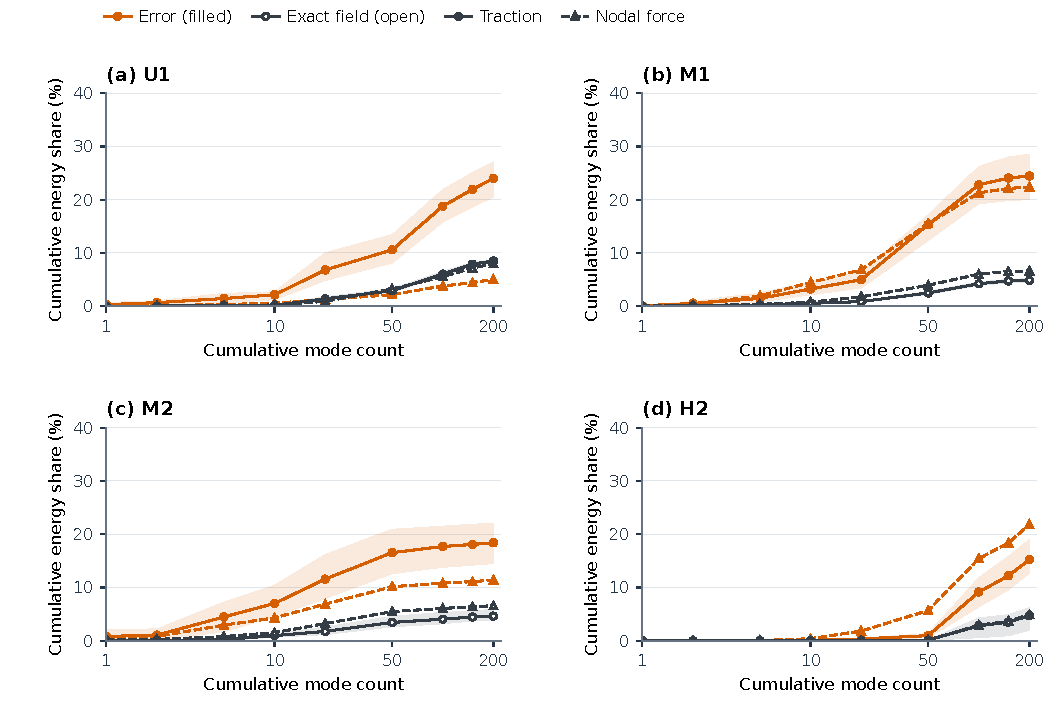
\includegraphics[width=\textwidth,height=0.8\textheight,keepaspectratio]{../figures/F03_spectrum.pdf}
\caption{\textbf{基础网络延拓误差的谱分布。} 各子图分别给出基础网络在 U1、M1、M2 和 H2 上的结果。模态求解 \(Av=\lambda Dv\)，其中 \(D=\operatorname{diag}(A)\)，并按特征值递增排序。深色实心标记表示延拓误差，浅灰色空心标记表示精确内部场；实线圆形对应一致面力，虚线三角形对应节点力。曲线为方向平均值；色带给出一致面力下第 10--90 方向百分位数。每条累积分数曲线均采用其自身场或误差的内部总能量。}\label{fig:5}
\end{figure}

在空间上（图 6），对于所绘的一致面力方向，M1 的精确场将其 8\% 的能量置于距切割面两个单元宽度以内的单元中，这些单元占全部单元的 13\%；在所评估的四个方向上，基础网络误差能量的 39--43\% 位于该层，紧邻保留切割带自由度，而延拓必须传播这些自由度的值。相对于基础网络，NICE 将总误差能量降低约两个数量级（113--138 倍），将单元误差能量降低约 25 至 300 倍（第 10--90 百分位数），并将该层所占份额减半至 19--22\%。

\begin{figure}[!htbp]
\centering
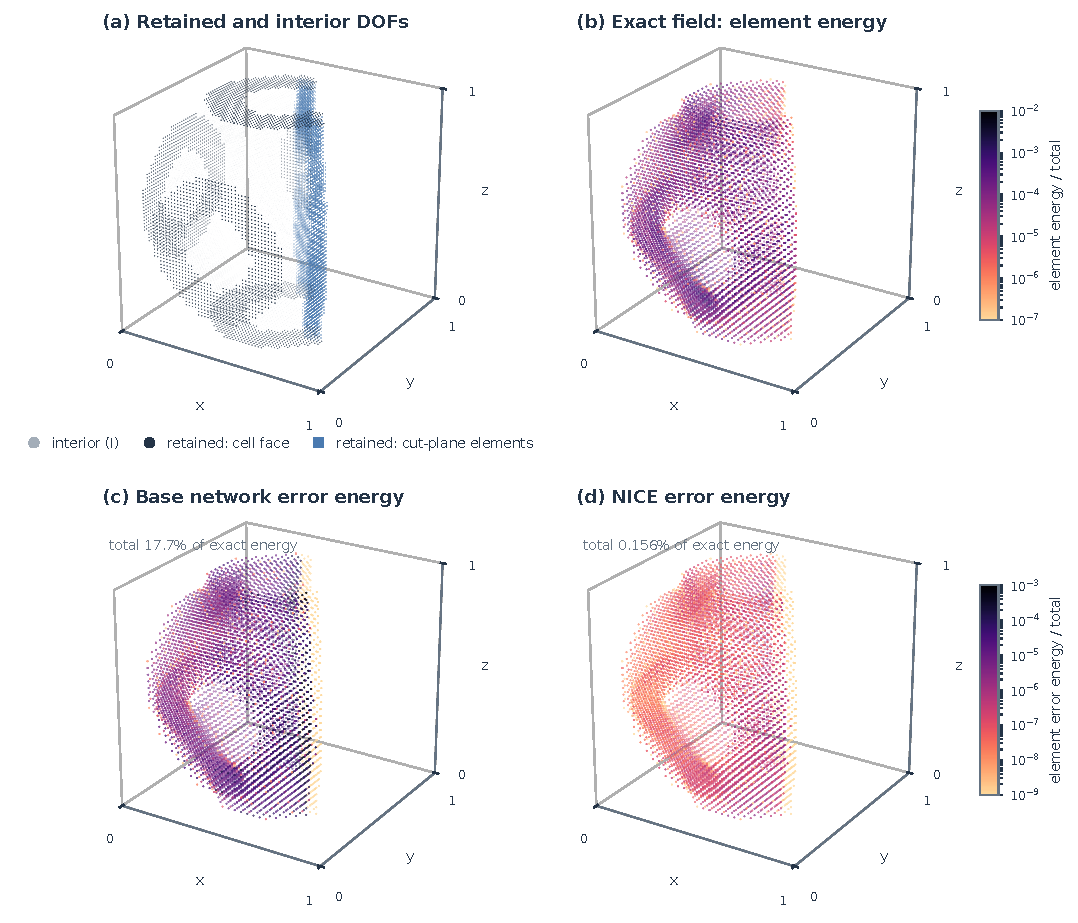
\includegraphics[width=\textwidth,height=0.8\textheight,keepaspectratio]{../figures/F12_field_error_M1.pdf}
\caption{\textbf{M1 中的保留自由度及延拓误差的空间分布。} (a) 保留盒面自由度、保留切割带自由度与内部自由度。(b) 一个一致面力方向下精确场的体单元能量，相对于其总能量。(c,d) 对相同保留位移，基础网络与 NICE 误差的体单元能量，相对于 (b) 中精确场的总能量，采用统一色标。切割带单元不含误差，因为其自由度是保留的。}\label{fig:6}
\end{figure}

这些能量误差的大小反映了一种可度量的放大效应。对于内部误差 \(d_I\) 和精确内部场 \(u_I\)，令 \(\delta^2=d_I^TDd_I/u_I^TDu_I\) 为 Jacobi 加权相对位移误差，\(\kappa=(d_I^TAd_I/d_I^TDd_I)/(u^TKu/u_I^TDu_I)\) 为内部误差与精确场的 Rayleigh 商之比。则在内部误差非零且精确内部场非零的每个方向上，\(\varepsilon=\delta^2\kappa\) 均精确成立（附录 B.3；数值见补充表 ST04）。在一致面力下，基础网络在 M1、M2、H1 和 H2 中的场平均 \(\delta\) 为 0.7--1.3\%，但平均 \(\kappa\) 为 124 至 7089：位移误差虽小，但其所在方向相对于自身幅值而言远比精确场刚硬，从而导致 1.8--35\% 的能量误差。在未切割的 U2 中，相近的 \(\delta\)（0.74\%）与 \(\kappa=85\) 相结合，得到 0.40\%；由于 \(\delta\)、\(\kappa\) 和 \(\varepsilon\) 是分别对方向取平均的，平均值的乘积不必等于平均误差（此处为 0.47\% 对 0.40\%）。NICE 的场在切割胞中 \(\delta\) 为 0.05--0.19\%，\(\kappa\) 为 33 至 582（U2 中分别为 0.11\% 和 47）。

在基础网络误差较大之处，式 (9) 的二次项占主导。在固定保留位移下，其平均能量误差和场基灵敏度误差在 M1 中为 13.5\% 和 14.1\%，在 H2 中为 35.0\% 和 75.1\%，而线性项仅占线性项与二次项范数之和的 7.2\%（M1）和 0.79\%（H2）。在其他情形下，线性项并不可忽略：在一致面力下，它在能量误差低于 2\% 的 U1、U2 和 H1 中占 28--43\%；在节点力下，它在所考察的全部六个胞（U1、U2、M1、M2、H1 和 H2）中占 24--72\%；由于线性项关于场误差是一阶的，当该误差趋于零时，它将占主导（表 ST05，图 S03）。

\subsection{在固定网络参数下降低内部误差}

保持基础网络固定，可单独考察校正的作用（图 7）。在固定保留位移下进行八步 Chebyshev 光滑，处处降低了平均能量误差，但降幅并不均匀（表 ST05a）：在一致面力下，H2 从 35.0\% 降至 0.205\%，而 M1 仅从 13.5\% 降至 4.69\%（32 步后为 2.95\%），因为其误差有很大一部分位于光滑区间以下的模态中（第 5.4 节）。M1 的灵敏度误差从 14.1\% 降至 2.76\%，而 U1 的灵敏度误差随步数非单调变化，尽管其能量误差每一步都在下降（图 7a,b）。

在相同的八步之前施加三线性粗网格校正，可使 M1 降至 0.230\%，再加八步前光滑则降至 0.186\%，其中粗自由度为 5,601 个，内部自由度为 165,927 个。每阶段两步、四步和八步在 M1 上分别得到 1.02\%、0.422\% 和 0.186\%，八步循环在 M2 和 U1 上约为 0.027\%（表 ST07）；其他粗空间的比较见表 ST06。

表 3 在相同的保留位移下，对四种初始场施加相同的校正：零内部场、图调和延拓（基于单元连接关系的体积加权图 Laplace 算子，采用相同的精确刚体分离）、基础网络的场以及 NICE。零内部场留下 28--1100\% 的能量误差，调和初始场留下 0.08--17\%，而基础网络的场最终为 0.004--0.19\%，比调和初始场低 7 至 290 倍，比零内部场低 2,400 至 12,000 倍。即使每阶段采用 64 步（即八倍的光滑工作量），在表 ST07 的六个胞（表 3 中的胞及 U1）中的五个上，调和初始场在一致面力下仍比基础网络的八步结果高 2.6 至 50 倍；仅在 H2 中达到该结果。由此可见，学习得到的场提供了光滑与粗空间在实际计算预算下无法达到的那部分内部平衡。

{\small
\begin{longtable}[]{@{}lrrrrr@{}}
\caption{对不同初始场施加相同的 8 / \(Q_1(17)\) / 8 校正后的平均能量误差（\%）（一致面力，32 个方向）}\tabularnewline
\toprule\noalign{}
胞 & 基础网络，无校正 & 零内部场 & 调和 & 基础网络（加校正） & NICE \\
\midrule\noalign{}
\endfirsthead
\toprule\noalign{}
胞 & 基础网络，无校正 & 零内部场 & 调和 & 基础网络（加校正） & NICE \\
\midrule\noalign{}
\endhead
\bottomrule\noalign{}
\endlastfoot
M1 & 13.5 & 1097 & 17.2 & 0.186 & 0.131 \\
M2 & 3.64 & 324 & 6.72 & 0.0273 & 0.0358 \\
H1 & 1.81 & 39.9 & 1.28 & 0.0131 & 0.0115 \\
H2 & 35.0 & 28.3 & 0.0806 & 0.0117 & 0.0148 \\
U2 & 0.402 & 47.2 & 1.23 & 0.00424 & 0.00465 \\
\end{longtable}}

第一列给出基础网络未经校正的误差。每阶段 16 至 64 步光滑的结果见表 ST07。

\begin{figure}[!htbp]
\centering
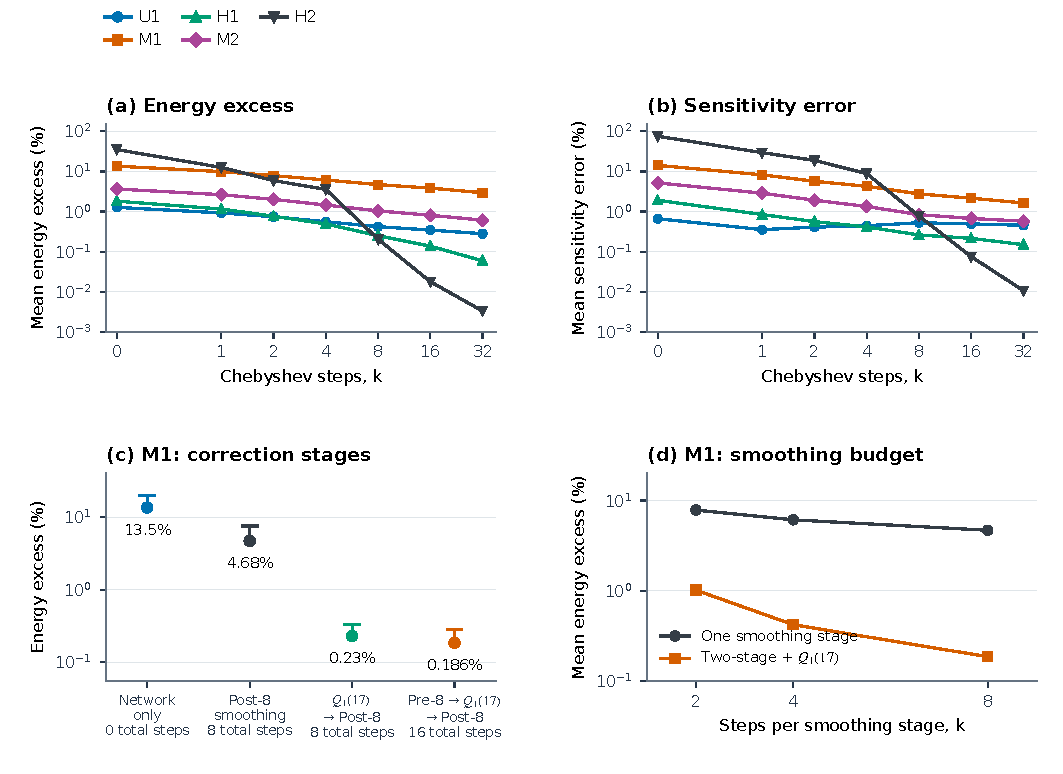
\includegraphics[width=\textwidth,height=0.8\textheight,keepaspectratio]{../figures/F04_correction.pdf}
\caption{\textbf{在固定网络参数下校正基础网络所获得的精度提升。} (a,b) 五个胞上 Chebyshev 光滑过程中的平均方向能量误差与场基灵敏度误差。(c) M1 在以下情形下的结果：无校正、八步光滑、粗网格校正后接八步光滑，以及粗网格校正前后各八步光滑；圆点表示平均值，端帽表示第 90 百分位数。(d) M1：平均能量误差随每个光滑阶段步数 \(k\) 的变化，分别对应单独一个光滑阶段，以及 \(k\) 步前光滑、\(Q_1(17)\) 粗网格校正与 \(k\) 步后光滑的组合。所有子图均采用一致面力、固定保留位移以及 \(a=b/30\)；在 (a,b) 中，步数轴在 0 到 1 之间为线性刻度，此后为对数刻度。}\label{fig:7}
\end{figure}

\subsection{装配后的柔度、局部灵敏度与能量份额}

第 5.3--5.5 节中较小的单胞能量误差，在胞装配后能否得到准确的柔度和局部灵敏度？两胞装配将一个学习的目标胞与一个精确的、未切割的邻胞连接，二者的厚度在界面处连续（图 8）。来自选择几何的七个目标胞为 U1、U2、L1、M1、M2、H1 和 H3，每个均有配置 x 和 y 两种情形；\textquotesingle M1/x\textquotesingle{} 表示配置 x 中的目标胞 M1。每种配置有六个面载荷，即三个笛卡尔面力方向分别施加于目标胞面和邻胞面。对于每个载荷，将柔度以及每个胞的厚度灵敏度（一个八分量向量）与其精确对应量进行比较，节点载荷固定为其基准设计值（载荷归一化与胞对求解器见补充说明 S4.2）。我们对柔度和每个胞的灵敏度向量统一采用 3\% 作为参考容差，在图中以 3\% 线绘出，并报告六个载荷上的最大值，对于灵敏度还取两个胞上的最大值。目标胞切割面上的三个面力单独考察。

\begin{figure}[!htbp]
\centering
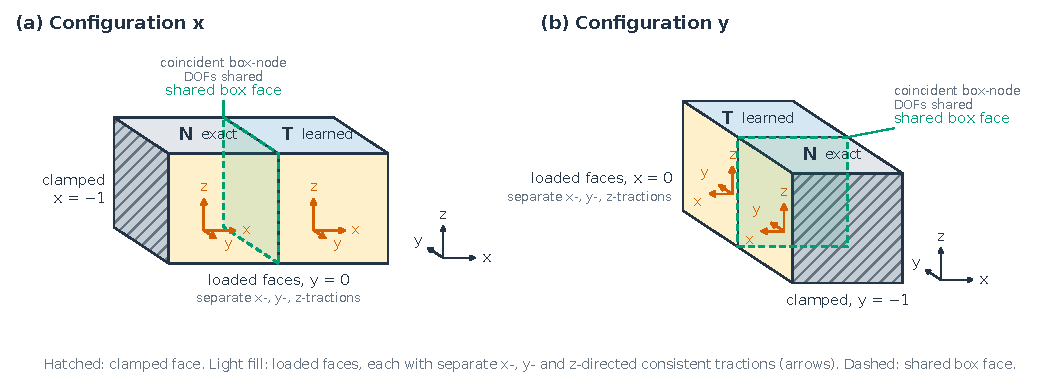
\includegraphics[width=\textwidth,height=0.8\textheight,keepaspectratio]{../figures/F09_assembly_loads.pdf}
\caption{\textbf{两胞装配的支撑与加载。} (a) 配置 x：邻胞平移 \((-1,0,0)\)，面 \(x=-1\) 固支，面力作用于 \(y=0\)。(b) 配置 y：平移为 \((0,-1,0)\)，面 \(y=-1\) 固支，面力作用于 \(x=0\)。目标胞（T）面与邻胞（N）面各自分别承受 x、y、z 方向的一致面力载荷。重合的盒节点自由度在界面上共享；非盒面的切割带自由度保持局部。切割目标胞还承受三个切割面面力，单独分析。}\label{fig:8}
\end{figure}

图 9 比较了各变体在这些配置中的表现。NICE 在七个选择胞的全部十四种配置中均低于两条 3\% 线：其在六个面载荷上的最大柔度误差为 0.056\%（M1/x），在两个胞上取最大的最大灵敏度误差为 0.67\%（U1/y）。厚度灵敏度向量的方向比其大小复现得更为精确：在这十四种配置中，NICE 的向量与精确向量的夹角余弦至少为 0.999998（补充说明 S4.3）。

在检查点选择之外的九个验证胞上，即 NICE 单胞误差最大的五个几何，以及在未切割、轻度、中度和重度切割分层中各随机选取的一个胞，十八种配置给出的最大值为柔度 0.27\%、灵敏度 1.49\%，二者均出现在单胞误差最大的几何上（补充表 ST08b）。所有高于 0.02\% 的柔度误差均来自这五个最大误差几何；四个分层胞分别保持在 0.011\% 和 0.22\% 以下。所有留出配置均低于两条 3\% 线。

未校正延续在其被评估的十一种配置中有四种超过 3\% 灵敏度线（U1/x、U1/y、M1/x、M1/y，最高 11.4\%；表 ST08），在 M1 上还超过柔度线（最高 4.1\%）。平滑训练降低了这些误差，但在同样的四种配置中仍超过该线（3.15--4.43\%）：不加粗网格校正的光滑会留下第 5.4 节中衰减缓慢的低阶模态误差，这与 U1 和 M1 中残留的灵敏度误差相一致。``基础网络（加校正）''同样低于两条线（最大灵敏度误差 0.95\%，U1/x），因此正是校正使装配响应降至两条线以下。

在切割面面力下，NICE 的柔度误差至多为 0.10\%（M1/y），灵敏度误差至多为 0.16\%；而未校正延续在其七种配置中有四种超过 3\% 线，其中包括在面载荷下低于该线的 M2/x（3.3\%）和 L1/y（3.7\%）；其最大误差出现在 M1/y 上，灵敏度为 14.1\%，柔度为 6.9\%（表 ST09）。

表 4 说明了为何两个量都是必需的。若无完整校正，准确的柔度并不能保证准确的局部灵敏度：在 U1/x 的一个邻胞面载荷下，平滑训练的柔度误差为 0.00109\%，而目标胞灵敏度误差为 3.15\%，此时目标胞承担精确装配能量的 0.13\%。NICE 降低了这两项误差：该载荷下的目标胞灵敏度误差降至 0.598\%；在 M1/x 的目标胞面 y 向载荷下，NICE 给出 0.0481\% 和 0.145\%，而未校正延续为 3.44\% 和 11.4\%。这种分离在 NICE 中依然可见：其灵敏度误差在 H1 上约为柔度误差的两倍，在能量份额较小的 U1 目标胞上则高出四个数量级，但二者均远低于 3\% 线。

\begin{figure}[!htbp]
\centering
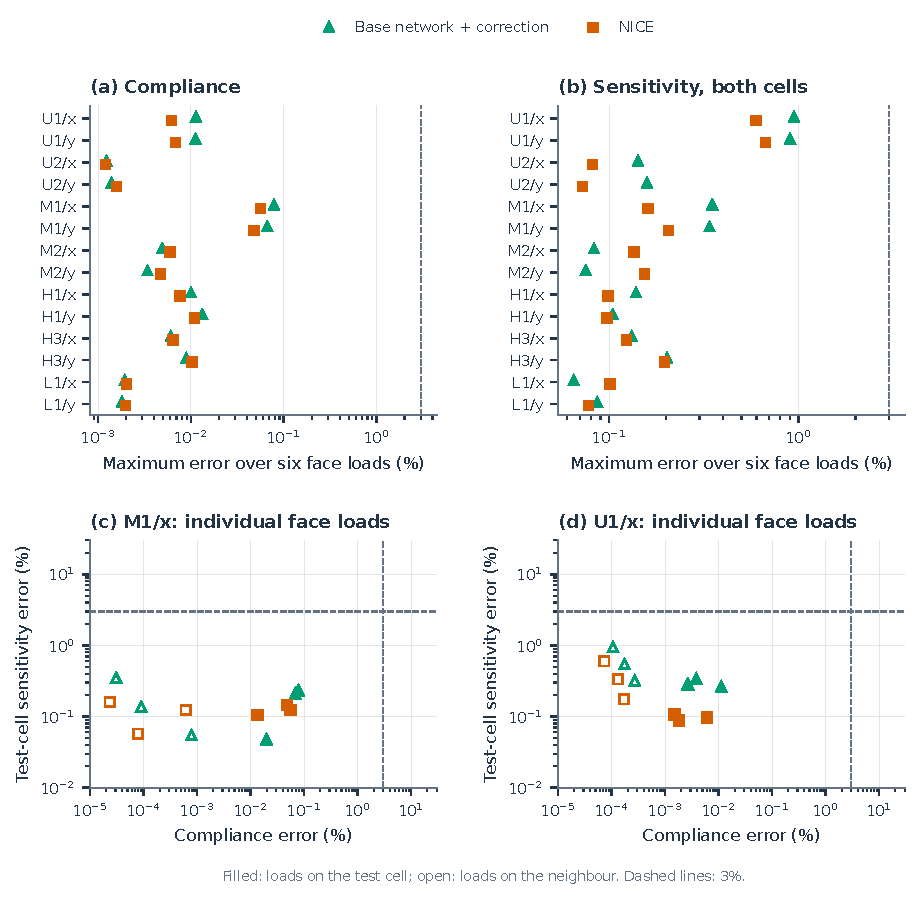
\includegraphics[width=\textwidth,height=0.8\textheight,keepaspectratio]{../figures/F05_assembly.pdf}
\caption{\textbf{两胞装配中的柔度与厚度灵敏度。} 目标胞由学习子结构表示，邻胞由精确凝聚表示。(a,b) 每种配置中六个面载荷上的最大误差；灵敏度误差还在两个胞上取最大。(c,d) M1/x 与 U1/x 上各单个面载荷的柔度误差与目标胞灵敏度误差；实心标记表示目标胞面载荷，空心标记表示邻胞面载荷。虚线标出 3\% 线。图中未显示基础网络，且并非每个变体都在每种配置上进行了评估；全部结果见表 ST08。变体同表 2；``基础网络（加校正）''指在部署时施加校正、未经重新训练的基础网络。}\label{fig:9}
\end{figure}

{\footnotesize
\begin{longtable}[]{@{}
  >{\raggedright\arraybackslash}p{(\linewidth - 10\tabcolsep) * \real{0.1579}}
  >{\raggedright\arraybackslash}p{(\linewidth - 10\tabcolsep) * \real{0.1579}}
  >{\raggedright\arraybackslash}p{(\linewidth - 10\tabcolsep) * \real{0.1579}}
  >{\raggedright\arraybackslash}p{(\linewidth - 10\tabcolsep) * \real{0.1579}}
  >{\raggedright\arraybackslash}p{(\linewidth - 10\tabcolsep) * \real{0.1579}}
  >{\raggedleft\arraybackslash}p{(\linewidth - 10\tabcolsep) * \real{0.2105}}@{}}
\caption{单个面载荷下的柔度与目标胞灵敏度}\tabularnewline
\toprule\noalign{}
\begin{minipage}[b]{\linewidth}\raggedright
目标胞 / 配置
\end{minipage} & \begin{minipage}[b]{\linewidth}\raggedright
载荷
\end{minipage} & \begin{minipage}[b]{\linewidth}\raggedright
未校正：柔度 / 灵敏度（\%）
\end{minipage} & \begin{minipage}[b]{\linewidth}\raggedright
平滑训练：柔度 / 灵敏度（\%）
\end{minipage} & \begin{minipage}[b]{\linewidth}\raggedright
NICE：柔度 / 灵敏度（\%）
\end{minipage} & \begin{minipage}[b]{\linewidth}\raggedleft
目标胞能量份额
\end{minipage} \\
\midrule\noalign{}
\endfirsthead
\toprule\noalign{}
\begin{minipage}[b]{\linewidth}\raggedright
目标胞 / 配置
\end{minipage} & \begin{minipage}[b]{\linewidth}\raggedright
载荷
\end{minipage} & \begin{minipage}[b]{\linewidth}\raggedright
未校正：柔度 / 灵敏度（\%）
\end{minipage} & \begin{minipage}[b]{\linewidth}\raggedright
平滑训练：柔度 / 灵敏度（\%）
\end{minipage} & \begin{minipage}[b]{\linewidth}\raggedright
NICE：柔度 / 灵敏度（\%）
\end{minipage} & \begin{minipage}[b]{\linewidth}\raggedleft
目标胞能量份额
\end{minipage} \\
\midrule\noalign{}
\endhead
\bottomrule\noalign{}
\endlastfoot
H1/x & T-x & 1.06 / 2.47 & 0.144 / 0.636 & 0.0076 / 0.0133 & 0.643 \\
U1/x & N-z & 0.0023 / 4.89 & 0.00109 / 3.15 & 7.3×10⁻⁵ / 0.598 & 0.0013 \\
M1/x & T-y & 3.44 / 11.4 & 1.14 / 4.43 & 0.0481 / 0.145 & 0.311 \\
\end{longtable}}

T 和 N 分别表示目标胞或邻胞的受载面；x、y 和 z 表示面力方向。最后一列给出目标胞在精确装配能量中所占的份额。

目标胞的能量份额（表 4）解释了局部刚度误差为何可能对柔度影响甚小。在 U1/x 的邻胞面 z 向载荷下，基础网络的目标胞承担精确装配能量的 0.127\%，局部能量误差为 2.31\%；二者之积 \(\beta=w\varepsilon\) 给出相对柔度界 0.00295\%，与观测值 0.00283\% 接近，而目标胞灵敏度误差为 5.83\%。图 10 展示了这种加权在各变体和各载荷中的情况。对于固定保留位移下的灵敏度，附录 H.1 用一个关于内部误差的线性项和一个二次项对误差加以界定；相对误差还需除以局部参考值，而对于承担装配能量很少的胞，该参考值很小。

\begin{figure}[!htbp]
\centering
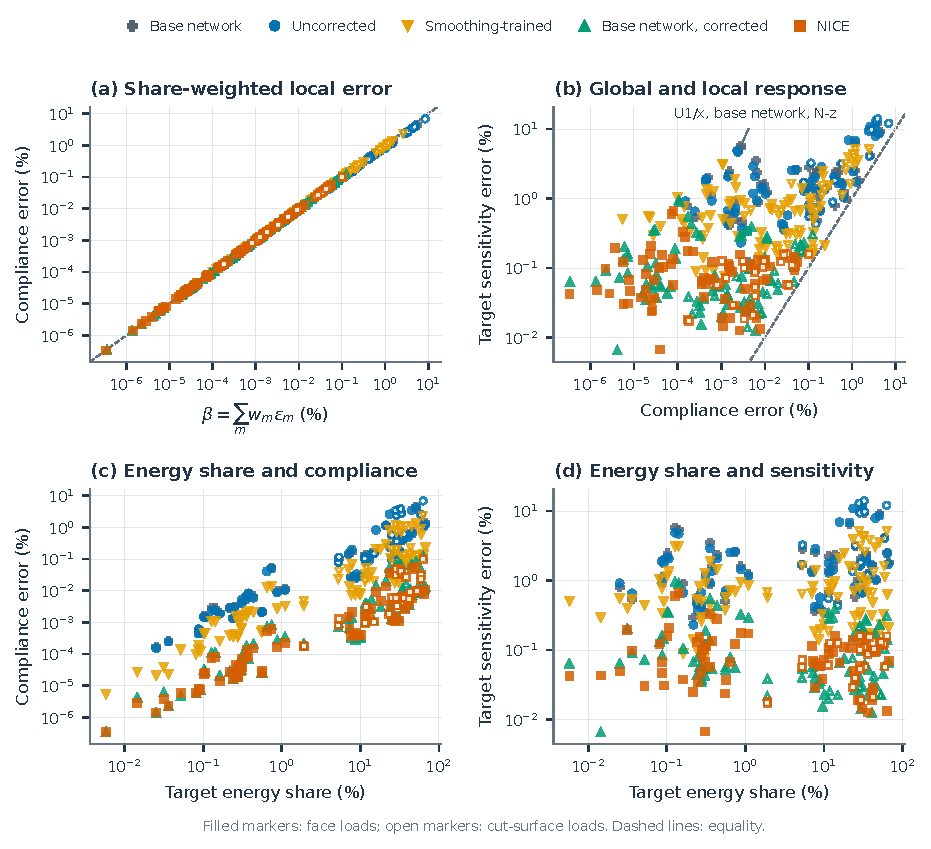
\includegraphics[width=\textwidth,height=0.8\textheight,keepaspectratio]{../figures/F10_energy_share.pdf}
\caption{\textbf{按份额加权的柔度误差与局部灵敏度。} 每个点对应某一变体--配置组合的一个载荷；各载荷上的最大值见表 ST08（面载荷）和表 ST09（切割面载荷）。实心标记表示面载荷，空心标记表示切割面载荷。(a) 柔度误差与 \(\beta=\sum_mw_m\varepsilon_m\) 的关系，其中能量份额 \(w_m=q_m^TS_mq_m/C\)，能量误差 \(\varepsilon_m=q_m^T(\widehat S_m-S_m)q_m/(q_m^TS_mq_m)\)，均在精确装配保留位移处计算；只有学习的目标胞对 \(\beta\) 有贡献。(b) 相同载荷下的柔度误差与目标胞灵敏度误差；标注指出 U1/x 上邻胞 z 向载荷下的基础网络。虚线表示相等。(c,d) 两项响应误差随目标胞精确能量份额的变化。变体同表 2 和图 9。}\label{fig:10}
\end{figure}

\subsection{消融：限制保留盒面表示}

为单独考察完整保留空间的作用，对配置 x 中的胞对采用精确胞算子求解，同时将每个胞的盒面位移限制为 \(r\) 次张量 Bernstein 多项式；非盒面切割带自由度仍不受限制。该消融仅在固定胞尺寸下限制现有胞的保留表示；缩减边界的学习子结构通过分区细化、边界增强或过采样来控制由此产生的误差 \href{https://doi.org/10.1016/j.jmps.2024.105893}{Huang et al. (2024)}, \href{https://doi.org/10.1016/j.cma.2026.118955}{Guo et al. (2026a)}, \href{https://arxiv.org/abs/2607.22019v1}{Guo et al. (2026b)}，本文不对其进行复现（补充说明 S2）。当所有盒面均受限时，一次多项式在 U1、M1、M2 和 H1 上给出 78--85\% 的柔度误差，在 \(r=5\) 时降至约 4\%，在 \(r=8\) 时降至 0.49--0.74\%；此时 H1 胞对的保留自由度为 14,001 个，而非 32,991 个（图 11）。

局部灵敏度收敛更慢：在 \(r=8\) 时，目标胞灵敏度误差在目标面载荷下为 1.3--4.5\%，在计入邻胞面载荷时为 24--64\%。仅限制共享界面即可消除大部分柔度误差（在 U1、M1 和 M2 上，\(r=3\) 时为 0.17--0.44\%），但邻胞载荷下的灵敏度误差在 \(r=3\) 时仍为 8--21\%，在 \(r=5\) 时仍为 2.2--3.4\%。因此，受限界面在低次时即足以满足柔度要求，却不足以满足邻胞载荷下的局部灵敏度要求；保留完整的保留空间可消除这部分误差，代价是粗模型规模更大（表 ST11）。

\begin{figure}[!htbp]
\centering
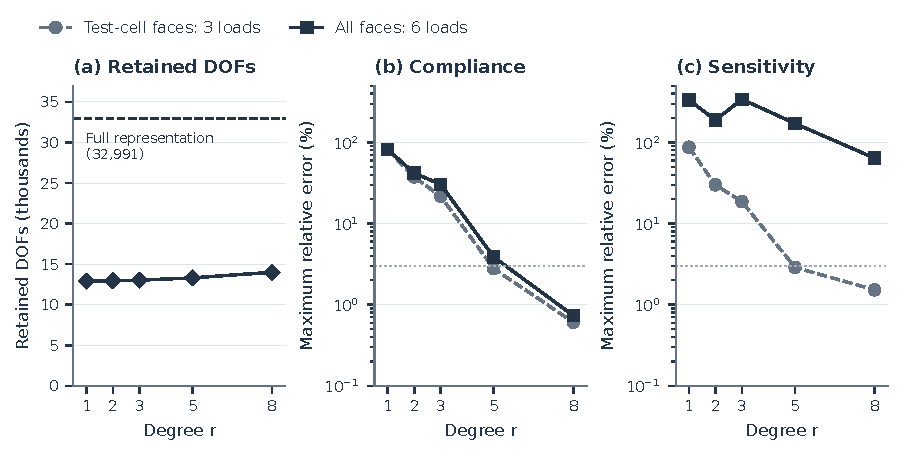
\includegraphics[width=\textwidth,height=0.8\textheight,keepaspectratio]{../figures/F06_bernstein.pdf}
\caption{\textbf{限制盒面位移引起的响应误差。} H1/x 的两个胞均采用精确算子，并在每个盒面上采用 \(r\) 次 Bernstein 多项式，非盒面切割带自由度不受限制。(a) 保留自由度数目；虚线表示完整表示的 32,991 个自由度。(b,c) 在三个目标面载荷或全部六个目标面与邻胞面载荷下的最大柔度误差和最大目标胞灵敏度误差；不计切割面面力。误差相对于完整保留空间解计算；水平线标示 3\%。}\label{fig:11}
\end{figure}

\subsection{所有胞均为学习胞的非均质格栅}

在设计中，每个胞都是学习得到的，相邻胞的误差会进入同一个装配解。为检验这一点，采用两个具有连续梯度厚度场和平面边界切割的格栅：一个由八个互不相同的胞组成的 \(2\times2\times2\) 块体，其中四个被切割，保留体积为 62\% 和 25\%；以及一个由八个胞组成的 \(3\times3\times1\) 层，其中三个被切割，并有一个角点位置留空。相邻胞共享其面角点，块体的角点参数范围为 0.25 至 0.54。这十六个胞专为这些算例生成，既未参与训练，也未参与检查点选择。格栅在一个面上固支，并在相对面上沿三个笛卡尔方向施加单位一致面力（面载荷），另施加三个随机载荷向量；计算灵敏度时，节点载荷保持为其在所评估设计处的值（附录 H）。每个胞均采用 NICE；参考解装配稠密的精确凝聚矩阵，并求解至重新计算的相对残差不超过 \(1.3\times10^{-10}\)。学习格栅在自由保留自由度上采用带平衡两层预条件子的预条件共轭梯度法求解：细层作用为装配保留刚度块 \(\mathbb K_{PP}=\sum_mB_m^TK_{PP,m}B_m\) 的逆，每次设计迭代分解一次；粗空间由三线性格栅顶点函数与六个刚体模态的乘积构成（补充说明 S4.1）。

在 \(2\times2\times2\) 块体中，三个面载荷下的格栅柔度误差分别为 0.014\%、0.011\% 和 0.0094\%（随机载荷下至多 0.069\%），所有胞中最大的厚度灵敏度误差为 0.14\%（随机载荷下为 0.45\%），装配保留解与精确解相差 0.13\%（全部六个载荷上的相对欧几里得范数）。\(3\times3\times1\) 层的相应结果为 0.015\%、0.013\% 和 0.010\%（至多 0.056\%），0.14\%（0.43\%）以及 0.12\%。格栅误差低于最大的两胞误差，这是因为式 (7) 以各胞在精确迹处的能量误差之和界定格栅柔度误差，并以各胞在装配能量中所占份额加权。在面载荷下，这些胞能量误差在块体中为 0.006\% 至 0.026\%，在层中为 0.005\% 至 0.052\%（随机载荷下为 0.02\% 至 0.12\%），且在切割胞中最大。加权和 \(\beta\) 超出格栅柔度误差的量在面载荷下小于 \(\beta\) 的 0.4\%，在随机载荷下约为 4--5\%，原因在于装配解会适应刚度更大的学习胞，而 \(\beta\) 是在精确迹处评估误差的。

学习求解在递推更新的残差上达到了规定容差，而重新计算的残差 \(\|f_g-\widehat{\mathbb K}\bar U\|/\|f_g\|\) 停滞于 \(3.6\times10^{-4}\)（块体）和 \(3.2\times10^{-3}\)（层），这与单精度网络中的舍入误差相符：在块体中，将校正由双精度改为单精度运行，对该残差的改变小于 1\%，因此校正并非其来源。最终迭代处的残差功 \(\bar U^T\rho\) 至多为柔度的 \(2.5\times10^{-8}\)。结合对偶范数界与作用--能量差异（补充说明 S4.3，表 ST14），这表明上述误差是算子的误差，而非不完全求解的误差。在共享角点参数上汇总后，场基灵敏度给出的格栅梯度在面载荷下误差为 0.04--0.09\%，在随机载荷下为 0.22--0.28\%，余弦值均高于 0.999999。

\subsection{含灵敏度的格栅分析的计算成本}

针对一次含灵敏度的格栅分析（从胞设置到求解）比较计算成本，所用格栅为第 5.8 节的两个八胞格栅，以及两个四胞格栅，即块体的两个 \(2\times2\times1\) 层。每层含两个未切割胞和两个保留体积分别为 62\% 和 25\% 的切割胞，并沿用块体的保留自由度、固支与载荷。表 5 比较了三种路线。

路线 (a) 为整体格栅直接求解：装配格栅的完整切割有限元模型（包括每个胞的保留自由度与内部自由度），并通过稀疏 Cholesky 分解（MKL PARDISO，在一颗 AMD EPYC 9654 CPU 上使用 16 线程）分解一次；其重新计算的相对残差低于 \(3\times10^{-9}\)，因此对于四胞格栅，它同时也是精确参考解。

路线 (b) 为常规精确凝聚：在同一 CPU 上，借助 PARDISO 的 Schur 补选项对每个胞的内部进行 Cholesky 分解以凝聚该胞，再通过块 Cholesky 分解求解装配后的凝聚系统，该分解先消去各胞私有的保留自由度，再消去共享界面（16 线程）；其柔度与 (a) 的吻合精度达 \(7\times10^{-10}\)。

路线 (c) 为在 GPU 上运行的 NICE：为每个胞准备学习子结构，采用第 5.8 节的预条件共轭梯度法将装配系统求解至相对残差 \(10^{-6}\)，并计算场基灵敏度；校正以单精度运行。

所有路线均包含胞设置与刚度装配，且均不包含数据生成与训练的一次性成本（第 5.1 节）。各路线运行于不同的处理器上，即一块 GPU 对比 16 个 CPU 线程；因此，比较的是各路线在各自部署方式下的表现，而非硬件等价的工作量。

{\footnotesize
\begin{longtable}[]{@{}
  >{\raggedright\arraybackslash}p{(\linewidth - 12\tabcolsep) * \real{0.120}}
  >{\raggedright\arraybackslash}p{(\linewidth - 12\tabcolsep) * \real{0.170}}
  >{\raggedright\arraybackslash}p{(\linewidth - 12\tabcolsep) * \real{0.160}}
  >{\raggedright\arraybackslash}p{(\linewidth - 12\tabcolsep) * \real{0.160}}
  >{\raggedright\arraybackslash}p{(\linewidth - 12\tabcolsep) * \real{0.130}}
  >{\raggedright\arraybackslash}p{(\linewidth - 12\tabcolsep) * \real{0.120}}
  >{\raggedright\arraybackslash}p{(\linewidth - 12\tabcolsep) * \real{0.140}}@{}}
\caption{一次含灵敏度的格栅分析的成本。 (a) 通过稀疏 Cholesky 分解进行整体格栅直接求解（MKL PARDISO，CPU 上 16 线程）：从胞设置到求解六个载荷（三个一致面力载荷、三个随机载荷）的时间；进程峰值内存。(b) 用 PARDISO 的 Schur 补选项凝聚每个胞，再通过块 Cholesky 分解求解凝聚后的格栅系统，16 线程：总时间、进程峰值内存。(c) 胞准备、预条件子设置、针对三个一致面力载荷求解至 \(10^{-6}\) 的共轭梯度迭代以及场基灵敏度；GPU 峰值内存、胞准备后的 CPU 内存；柔度误差对四胞格栅相对于 (a) 计算，对八胞格栅相对于第 5.8 节的精确凝聚计算。内存单位为 GiB。所有阶段：补充说明 S3 与表 ST12。}\tabularnewline
\toprule\noalign{}
\begin{minipage}[b]{\linewidth}\raggedright
格栅（切割胞数 / 胞数）
\end{minipage} & \begin{minipage}[b]{\linewidth}\raggedright
自由度：总数 / 自由保留
\end{minipage} & \begin{minipage}[b]{\linewidth}\raggedright
(a) 整体格栅直接求解，16 线程：时间 (s) / 内存 (GiB)
\end{minipage} & \begin{minipage}[b]{\linewidth}\raggedright
(b) 常规精确凝聚，16 线程：时间 (s) / 内存 (GiB)
\end{minipage} & \begin{minipage}[b]{\linewidth}\raggedright
(c) NICE（单 GPU）：时间 (s) / 迭代次数
\end{minipage} & \begin{minipage}[b]{\linewidth}\raggedright
(c) NICE 内存 (GiB)：GPU / CPU
\end{minipage} & \begin{minipage}[b]{\linewidth}\raggedright
(c) NICE 柔度误差 (\%)
\end{minipage} \\
\midrule\noalign{}
\endfirsthead
\toprule\noalign{}
\begin{minipage}[b]{\linewidth}\raggedright
格栅（切割胞数 / 胞数）
\end{minipage} & \begin{minipage}[b]{\linewidth}\raggedright
自由度：总数 / 自由保留
\end{minipage} & \begin{minipage}[b]{\linewidth}\raggedright
(a) 整体格栅直接求解，16 线程：时间 (s) / 内存 (GiB)
\end{minipage} & \begin{minipage}[b]{\linewidth}\raggedright
(b) 常规精确凝聚，16 线程：时间 (s) / 内存 (GiB)
\end{minipage} & \begin{minipage}[b]{\linewidth}\raggedright
(c) NICE（单 GPU）：时间 (s) / 迭代次数
\end{minipage} & \begin{minipage}[b]{\linewidth}\raggedright
(c) NICE 内存 (GiB)：GPU / CPU
\end{minipage} & \begin{minipage}[b]{\linewidth}\raggedright
(c) NICE 柔度误差 (\%)
\end{minipage} \\
\midrule\noalign{}
\endhead
\bottomrule\noalign{}
\endlastfoot
\(2\times2\times1\), \(z=0\) (2 / 4) & 957,888 / 77,310 & 484 / 35.1 & 589 / 27.9 & 39.4 / 114 & 6.3 / 2.4 & 0.015, 0.012, 0.010 \\
\(2\times2\times1\), \(z=1\) (2 / 4) & 884,940 / 71,046 & 349 / 32.0 & 632 / 24.7 & 37.3 / 119 & 6.1 / 2.4 & 0.022, 0.016, 0.014 \\
\(2\times2\times2\) (4 / 8) & 1,833,474 / 139,002 & 868 / 71.1 & 950 / 40.1 & 79.2 / 129 & 8.5 / 3.9 & 0.014, 0.011, 0.0097 \\
\(3\times3\times1\) (3 / 8) & 2,113,611 / 143,685 & 1,042 / 85.9 & 1,218 / 42.2 & 105.5 / 164 & 9.2 / 4.7 & 0.015, 0.014, 0.015 \\
\end{longtable}}

对于四胞格栅，一次 NICE 分析耗时 37 至 39 s，而 16 线程的整体格栅直接求解需 349 至 484 s，常规精确凝聚需 589 至 632 s；学习柔度与直接求解结果的吻合在 0.022\% 以内。对于两个八胞格栅，NICE 每次分析分别耗时 79 s 和 105 s；整体格栅直接求解耗时 868 s 和 1,042 s，约为其十倍，常规精确凝聚耗时 950 s 和 1,218 s。使用 32 线程时，直接求解仍需 341 至 956 s，仅略少于 16 线程，原因是胞设置与装配并未随之加速（补充表 ST12b）。若按全尺度比较中常见的报告方式以单线程运行，直接求解耗时 2,131 至 8,131 s，为 NICE 的 57 至 77 倍（补充表 ST12b）。在路线 (a) 中，CPU 上的胞设置与刚度装配占总时间的 41 至 53\%。扣除这两部分后，直接求解耗时 165 至 610 s；扣除 NICE 在 GPU 上的胞准备（除设置与装配外，还包括网络编码与校正设置）后，NICE 耗时 31 至 93 s，快五至八倍。对于八胞格栅，计时所得的柔度误差包含 \(10^{-6}\) 求解的代数误差（式 (8)），比第 5.8 节的算子误差至多高 0.005 个百分点。

Cholesky 因子的增长略快于自由度数，从四胞时的 29 至 32 GiB 增至八胞时的 66 GiB 和 81 GiB，直接求解的进程峰值达到 71 GiB 和 86 GiB；常规精确凝聚需要 40 GiB 和 42 GiB，其中大部分用于存放在被消去之前一直保留的凝聚胞矩阵（补充表 ST12）。NICE 的 GPU 内存峰值为 9.2 GiB，胞准备后占用 4.7 GiB 的 CPU 内存。按单个胞计，NICE 存储的状态占用 0.25 至 1.37 GiB，而常规精确凝聚的内部 Cholesky 因子占用 0.60 至 9.4 GiB（补充说明 S3，表 ST13）。

在设计迭代中，每个胞的几何都会改变，因此每个胞的准备工作（其内部分解，或其网络编码与校正设置）都需重复进行，与表 5 中的分析相同；装配求解可以从前一个解出发，而在活动单元模式不变时，常规路线可以复用其符号分解。

\subsection{厚度设计优化}

本节优化两个算例：算例 A，即第 5.8 节的 \(2\times2\times2\) 块体；以及一块切割面固支板。二者均在下文描述。位于格栅顶点的角点厚度参数汇集于全局向量 \(\boldsymbol\tau_g\) 中，并通过 \(\boldsymbol\tau_m=\boldsymbol\tau_m(\boldsymbol\tau_g)\) 映射到各胞的角点；在单个单位一致面力作用下，以柔度最小为目标对其进行优化，约束为 \(V\le V^*=0.8\,V(\boldsymbol\tau^0)\)，其中 \(V\) 为离散模型的材料体积。位于加载面所在平面内的顶点参数（算例 A 中 27 个中的 9 个，板中 74 个中的 10 个）保持固定，这使节点载荷与设计无关，并消除了附录 H 中的载荷导数项 \(2f_{g,c}^T\widehat U\)。优化器接收式 (9) 的场基估计在每个顶点处对相关胞的求和，即 \(\sum_m(\partial\boldsymbol\tau_m/\partial\boldsymbol\tau_g)^T\widetilde{\boldsymbol s}_m\)。界限 \(0.18\le\tau\le0.69\)，以及对每个胞角点跨度和梯度范数所设的 0.45 限值，使每个胞都保持在训练域内（{[}0.175, 0.699{]}，至多 0.47；第 6.4 节）。每次设计迭代都会重新生成每个胞的几何与学习子结构，从前一个解出发用第 5.8 节的预条件共轭梯度法求解格栅，并采用移动渐近线法 \href{https://doi.org/10.1002/nme.1620240207}{Svanberg (1987)}（Svanberg (2007) 的变体）执行一步更新，移动限为参数范围的 5\%，且不进行线搜索（表 ST16）。

算例 A 为第 5.8 节的 \(2\times2\times2\) 块体，在与固支面相对的面上施加法向面力；从其梯度设计出发，分别用 NICE 以及作为对照的精确凝聚进行优化（孪生运行；表 6，图 12a）。NICE 在 24 次设计迭代后停止，精确凝聚在 23 次后停止，二者的停止条件均为目标函数的相对变化连续三次迭代保持低于 \(10^{-4}\)（表 ST16）；由于离散模型及其目标函数在设计迭代之间会发生变化（第 3.3 节，补充说明 S6.1），停止判据未采用 Karush--Kuhn--Tucker（KKT）残差。二者均在材料减少 20\% 的同时使柔度降低 2.0\%；其最终角点参数之差至多为 0.0051，最终设计的精确柔度之差为其值的 \(1.25\times10^{-5}\)。在第 0、12 和 23 次迭代时，NICE 柔度分别比精确值低 0.011\%、0.018\% 和 0.028\%，其符号由式 (7) 给出；格栅梯度的误差分别为 0.069\%、0.17\% 和 0.33\%，余弦值至少为 0.999996，逐变量误差的第 95 百分位数至多为最大分量的 0.28\%，且每个分量的符号均与精确值一致（表 ST17）。两类误差均随设计趋近界限而增大，但最终的 NICE 设计在每个角点参数上仍与孪生设计吻合至 0.0051 以内。

切割面固支板为单层 \(8\times4\) 胞，经平面切割去除其中八个后，剩余 16 个未切割胞和八个切割胞（补充说明 S6.3）。该板在其切割面上固支：每个切割胞切割带的所有自由度均被固定；这一支撑位于距切割面一个单元（\(h=1/32\)）的范围内，保留切割带无需重新训练即可表示它。其端面宽四个胞，承受合力为单位值的一致面力，方向位于板平面内并垂直于其长边，从而使板成为沿斜向切割面支撑的面内悬臂（图 13a）。切割法向（\(\vartheta=33.7^\circ\)）处于 NICE 主要评估的取向范围内（\(0<\vartheta<\pi/4\)，第 5.1 节和第 6.4 节）。

从均匀的 \(\tau=0.40\) 出发，NICE 按目标变化准则在 24 次设计迭代后停止（图 12b）。在体积减小至 \(V^*\) 的过程中，柔度由 75.59 升至 110.49，随后降至 78.26；最终设计同时触及上下界以及跨度和梯度限值，其最厚的壁位于支撑靠近加载面的一端附近以及对侧自由边沿线，而远离载荷的胞被减薄至下界（图 13a）。经精确凝聚校核（表 ST21），NICE 柔度在均匀初始设计处比精确值低 0.011\%，在最终设计处低 0.030\%；格栅梯度的误差为 0.029\% 和 0.30\%，余弦值至少为 0.999996，逐变量误差的第 95 百分位数至多为最大分量的 0.27\%，且全部 64 个分量的符号均与精确值一致。

参照基于均匀化的梯度设计 \href{https://doi.org/10.1016/j.cad.2018.06.003}{Li et al. (2018)}，建立一个均匀化模型，其张量取自在同一离散模型上通过周期均匀化得到的均匀厚度胞（表 ST18b）；该模型在切割平面上固支，并采用相同的变量、界限、限值、体积约束和优化器进行优化；其体积由均匀化材料体积分数 \(V^H(\tau)\) 计算，在均匀初始设计处与离散材料体积的吻合精度达 \(1.2\times10^{-7}\)。该模型将均匀初始设计的精确柔度低估了 27.0\%，这与单层结构在厚度方向上不存在尺度分离相符；沿其自身优化路径，其柔度比 NICE 柔度低 27--33\%；直至第 3 次迭代，两次运行分析的是相同的设计（图 12b）。在切割几何上分析时，均匀化设计少用 0.18\% 的材料，柔度却比 NICE 设计高 2.44\%；无论二者均用 NICE 还是均用精确凝聚评估，该差异都相同（精确柔度为 80.198 和 78.287；表 ST18c 和表 ST21）。其角点参数与 NICE 设计的差异可达 0.26（相关系数 0.95；表 ST18c，图 13b）。因此，均匀化模型对切割层响应的误判达 27\%，并导致在切割几何上刚度较低的设计；要预测切割层的响应并对其进行优化，需要采用切割胞模型。

在每一对相邻设计迭代之间，离散模型均发生了切换（第 3.3 节）：算例 A 的 8 个胞中至少 3 个、板的 24 个胞中至少 11 个发生切换（表 ST19b）；式 (8) 的残差功始终至多为柔度的 \(5.4\times10^{-8}\)。在所有运行中，共有四次设计迭代需要几何生成器对某个角点参数施加至多 \(5.8\times10^{-4}\) 的扰动（补充表 ST19a 及补充说明 S6.4）。一次 NICE 设计迭代对算例 A 平均耗时 74 s，对板平均耗时 200 s（155--270 s），板的 24 次迭代共耗时 1.3 h（表 6，补充表 ST18a）。

为考察成本随格栅规模的增长情况，在与该板比例和切割方式相同、分别含 24、51、88 和 110 个胞的板上对设计迭代进行计时；这些板沿未切割的长边固支，并在相对面上施加面内载荷（图 13c，表 ST20）。它们含 8 至 18 个切割胞，切割有限元模型含 650 万至 3270 万个自由度，凝聚后为 39 万至 162 万个自由保留自由度；每块板运行其前四次设计迭代，超出 4 GiB GPU 内存的学习子结构从 CPU 内存流式传输。一次设计迭代分别耗时 4.0、9.1、16.0 和 19.4 min，与胞数成正比（每胞 10.1 至 10.9 s），共轭梯度迭代次数为 138 至 173。CPU 内存存放学习胞的流式状态，每增加一个胞约增长 0.7 GiB；在学习胞驻留于 GPU 上固定的 4 GiB 内存中的情况下，GPU 内存随装配保留系统增长，预条件子直接分解该系统的刚度 \(\mathbb K_{PP}\)（表 ST20）。

{\scriptsize
\begin{longtable}[]{@{}
  >{\raggedright\arraybackslash}p{(\linewidth - 14\tabcolsep) * \real{0.110}}
  >{\raggedright\arraybackslash}p{(\linewidth - 14\tabcolsep) * \real{0.070}}
  >{\raggedright\arraybackslash}p{(\linewidth - 14\tabcolsep) * \real{0.170}}
  >{\raggedleft\arraybackslash}p{(\linewidth - 14\tabcolsep) * \real{0.070}}
  >{\raggedleft\arraybackslash}p{(\linewidth - 14\tabcolsep) * \real{0.100}}
  >{\raggedleft\arraybackslash}p{(\linewidth - 14\tabcolsep) * \real{0.100}}
  >{\raggedright\arraybackslash}p{(\linewidth - 14\tabcolsep) * \real{0.240}}
  >{\raggedleft\arraybackslash}p{(\linewidth - 14\tabcolsep) * \real{0.080}}@{}}
\caption{厚度优化算例。 单位一致面力下的柔度。初始：初始设计，其体积在每次运行中均比 \(V^*\) 高 25\%；最终：最后一次设计迭代。除特别标注外，柔度均为 NICE 值。精确校核：各设计的精确离散柔度，括号内为 NICE 柔度低于该值的幅度。迭代次数：设计迭代次数。时间：一次设计迭代的平均时间，包括每个胞的几何生成。与表 5 中的分析不同，一次设计迭代需重新生成每个胞的几何，并针对一个载荷求解（补充说明 S6.1）。Hom：均匀化宏观模型（4,464 个三线性单元）。详见补充说明 S6 及表 ST16--ST21。}\tabularnewline
\toprule\noalign{}
\begin{minipage}[b]{\linewidth}\raggedright
算例
\end{minipage} & \begin{minipage}[b]{\linewidth}\raggedright
胞数（切割）
\end{minipage} & \begin{minipage}[b]{\linewidth}\raggedright
支撑与载荷
\end{minipage} & \begin{minipage}[b]{\linewidth}\raggedleft
迭代次数
\end{minipage} & \begin{minipage}[b]{\linewidth}\raggedleft
初始 \(C\)
\end{minipage} & \begin{minipage}[b]{\linewidth}\raggedleft
最终 \(C\)
\end{minipage} & \begin{minipage}[b]{\linewidth}\raggedright
精确校核
\end{minipage} & \begin{minipage}[b]{\linewidth}\raggedleft
时间 (s)
\end{minipage} \\
\midrule\noalign{}
\endfirsthead
\toprule\noalign{}
\begin{minipage}[b]{\linewidth}\raggedright
算例
\end{minipage} & \begin{minipage}[b]{\linewidth}\raggedright
胞数（切割）
\end{minipage} & \begin{minipage}[b]{\linewidth}\raggedright
支撑与载荷
\end{minipage} & \begin{minipage}[b]{\linewidth}\raggedleft
迭代次数
\end{minipage} & \begin{minipage}[b]{\linewidth}\raggedleft
初始 \(C\)
\end{minipage} & \begin{minipage}[b]{\linewidth}\raggedleft
最终 \(C\)
\end{minipage} & \begin{minipage}[b]{\linewidth}\raggedright
精确校核
\end{minipage} & \begin{minipage}[b]{\linewidth}\raggedleft
时间 (s)
\end{minipage} \\
\midrule\noalign{}
\endhead
\bottomrule\noalign{}
\endlastfoot
A，NICE & 8 (4) & 固支面；相对面上施加法向面力 & 24 & 24.5908 & 24.1038 & 第 0、12、23 次迭代：24.5936 (0.011\%)、26.0063 (0.018\%)、24.1105 (0.028\%) & 74 \\
A，精确凝聚 & 8 (4) & 同 A & 23 & 24.5936\(^{a}\) & 24.1108\(^{a}\) & 全程精确；最终设计比 NICE 设计高 0.0013\% & 469 \\
板，NICE & 24 (8) & 固支切割带；端面上施加面内面力 & 24 & 75.591 & 78.264 & 第 0、23 次迭代：75.599 (0.011\%)、78.287 (0.030\%) & 200 \\
板，Hom & 宏观尺度 & 同板 & 23 & 55.19\(^{b}\)（NICE 75.59） & 55.27\(^{b}\)（NICE 80.17） & 最终设计：80.198 (0.032\%) & 4\(^{b}\) \\
规模：24、51、88、110 个胞的板 & 24--110 (8--18) & 固支长边；相对面上施加面内面力 & 4 次计时 & 94.34, 89.12, 86.75, 85.38 & --- & 未校核 & 242; 547; 962; 1,164 \\
\end{longtable}}

\(^{a}\) 精确柔度。\(^{b}\) 均匀化宏观模型（CPU 上的时间）；括号内为同一设计在切割几何上的 NICE 柔度。

\begin{figure}[!htbp]
\centering
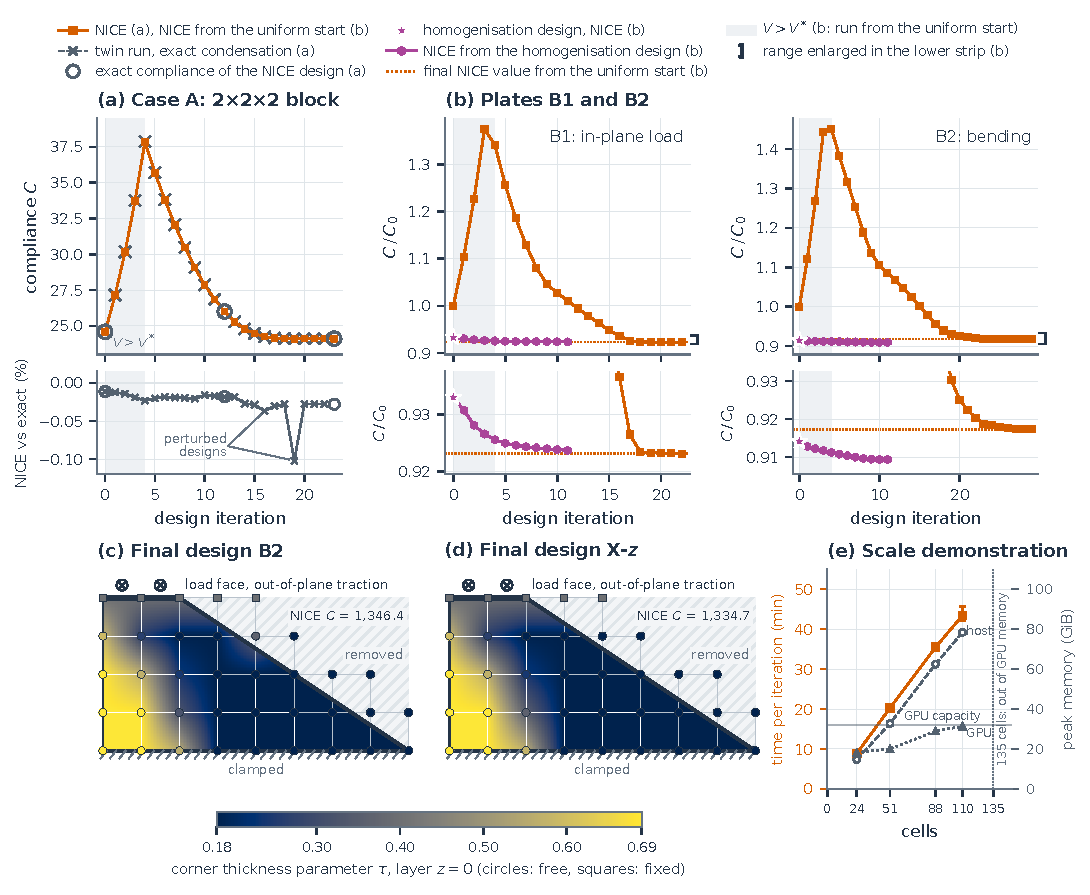
\includegraphics[width=\textwidth,height=0.8\textheight,keepaspectratio]{../figures/F13_optimisation.pdf}
\caption{\textbf{基于 NICE 的厚度优化。} (a) 算例 A：NICE 优化与采用精确凝聚的孪生优化的柔度历程，以及 NICE 设计在第 0、12 和 23 次迭代时的精确柔度（空心圆）；在体积由 \(1.25V^*\) 减小至 \(V^*\) 的过程中（阴影，第 0--3 次迭代），柔度先上升。下方条带：NICE 柔度相对于同一设计迭代处孪生运行的偏差（线；两次运行的设计在第 0--4 次迭代时重合，此后不同），以及相对于同一设计精确柔度的偏差（圆：−0.011\%、−0.018\%、−0.028\%）；在第 16 和 19 次迭代（标注为 \textquotesingle perturbed designs\textquotesingle），几何生成的回退机制对 NICE 设计施加了扰动（补充说明 S6.4，表 ST19a）。(b) 切割面固支板：从均匀初始设计出发的 NICE 柔度、均匀化宏观模型沿其自身优化路径的柔度（虚线）、在切割几何上用 NICE 分析的均匀化设计（星号，位于最后一次宏观迭代处），以及均匀初始设计、最终 NICE 设计和均匀化设计的精确柔度（空心圆）。阴影：\(V>V^*\) 的设计迭代。下方条带：括号所标范围的放大，自第 15 次迭代起。}\label{fig:12}
\end{figure}

\begin{figure}[!htbp]
\centering
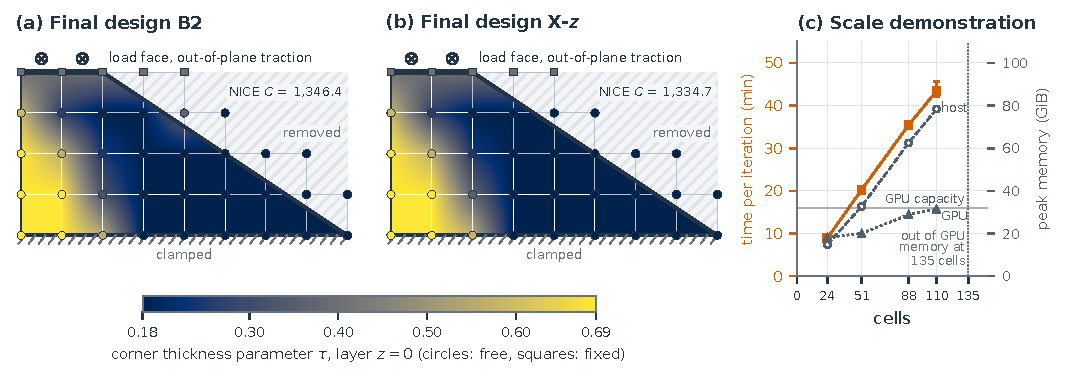
\includegraphics[width=\textwidth,height=0.8\textheight,keepaspectratio]{../figures/F14_designs_scale.pdf}
\caption{\textbf{板设计与规模演示。} (a,b) 最终 NICE 设计与均匀化设计的角点厚度参数，长边水平绘制，层 \(z=0\)；圆：设计变量；方块：位于加载面平面内、保持固定的顶点；绘于移除区域内的顶点为切割胞的角点。带阴影线的粗线：固支切割带；箭头：加载面及面内面力方向。(c) 在与 (a,b) 中板比例和切割方式相同、沿未切割长边固支并在相对面上施加面内载荷的板上进行的规模演示：每次设计迭代的时间（平均值；误差条：各计时迭代的范围）随胞数的变化；虚线：按每胞平均时间的正比关系；内存见表 ST20。(a,b) 中的柔度：同一设计的 NICE 值与精确值（表 ST21）。}\label{fig:13}
\end{figure}

\section{讨论}

\subsection{保留什么、如何表示以及校正什么}

固定保留自由度，可将约化子结构模型中原本合二为一的两项决策分离开来：相邻胞之间可以交换哪些位移模式，以及内部对其中每一种模式的响应有多精确。学习与校正只改变后者。第 5.7 节的消融实验表明了前者的作用：即便内部是精确的，限制盒面位移也会改变装配后的响应，而且一个能给出准确柔度的次数仍可能留下可观的灵敏度误差。在所考察的切割胞中，在胞尺寸固定、且不采用约化边界方法所用的分区加密或富集的情况下，限制盒面表示所产生的局部灵敏度误差大于 NICE 的内部近似所产生的误差（第 5.6 和 5.7 节，针对两胞装配）。保留的切割带使切割面上的载荷与支撑无需重新训练即可施加：在切割面无面力的格栅中，其位于盒面之外的自由度占自由保留自由度的 37\% 至 50\%（表 ST12a）；第 5.10 节的板即通过切割带固支，而对于这种支撑，均匀化模型需要在切割平面上另行施加约束。

正是这种表示使完整保留空间变得可学习。作用于模板、通道和网格层级上的权重，使一个约 \(6\times10^5\) 个参数的网络即可服务于含 2,679 至 45,900 个自由度的保留集；对保留位移的精确线性通过构造给出了叠加性、容许性和刚体再现（式 (17)）；并且由于该算子无需显式形成即可施加，每个胞存储的是由其几何所决定的量，而非其保留自由度上的稠密矩阵（第 4.6 节）。这种通用性的代价是网络与其训练所用的离散绑定：其每个坐标轴 65、33、17 和 9 个位置的潜在层级与 \(n=32\) 相匹配，换用其他分辨率需要重新训练（第 6.4 节）。

在内部，预测与校正相辅相成，而二者之间的分工正是由变分结构揭示出来的。对于任意保留输入都不增大 \(A\)-能量误差的内部校正，都会得到介于未校正凝聚刚度与精确 Schur 补之间的凝聚刚度，且与网络无关（第 4.3 节）。约百分之一的位移误差之所以变为 1.8\% 至 35\% 的能量误差，是因为误差比解更``刚''（第 5.4 节）；光滑消除缩放内部算子 Rayleigh 商较大的分量，粗网格校正则消除光滑迭代难以快速触及的平滑分量。学习场提供了二者在实际预算下都无法达到的部分：在相同校正下，在表 3 的五个胞上，调和初值留下的误差是学习场的 7 至 290 倍，而将光滑工作量增至八倍也仅在六个胞中的一个上弥合了这一差距。反过来，校正也替网络承担了其难以表示的部分：M1 上 13.5\% 的基础网络误差在不改变任何网络参数的情况下降至 0.19\%，且``基础网络（加校正）''在两胞配置中已保持在 3\% 线以下，因此现有网络无需重新训练即可从校正中获益。经由校正进行训练所带来的增益小于校正本身，仅为进一步的 1.31 倍（第 5.3 节）。

\subsection{保证的覆盖范围}

变分性质对任意输入均成立；在粗求解精确或经非负平移（附录 F.1）的条件下，排序关系对谱位于光滑区间上端以下的每个几何均成立（第 5.2 节）。设计求导引入了一项能量误差无法控制的额外要求。在公共保留向量 \(q\) 处，令 \(H=J_I(F-E)\)（同式 (4)）、\(E_{I,c}=J_IE_{,c}\)、\(H_{,c}=\partial H/\partial\tau_c\) 以及 \(K_{II,c}=J_IK_{,c}J_I^T\)，由式 (9) 和式 (10) 可得（附录 H.2，式 (H.5)）
\[
\widetilde s_c-s_c=2(Hq)^TAE_{I,c}q-(Hq)^TK_{II,c}Hq,\qquad
-q^T\widehat S_{,c}q-s_c=-2(H_{,c}q)^TA\,Hq-(Hq)^TK_{II,c}Hq,
\]
其中第一式在公共 \(q\) 处成立，第二式在式 (10) 的装配 \(\widehat q\) 处成立。因此，式 (10) 中的残差项消去了线性场误差项，并代之以一个由延拓误差的设计导数加权的项。两者中哪一个是更准确的梯度，取决于 \(\|H_{,c}q\|_A\) 相对于 \(\|E_{I,c}q\|_A\) 是否较小。对 \(\widehat C_{,c}\) 的中心差分检验无法回答这一问题：在每个格栅胞的 49 次重建中，有 21 至 48 次至少发生了第 3.3 节所列离散选择之一的切换，且差商随步长减小而增大（补充说明 S4.3，表 ST14）。场基估计无需差商，对第 5.8 节的两个八胞格栅以及块体的两个四胞层（第 5.9 节），其共享变量梯度的精度在面载荷下为 0.02--0.13\%，在随机载荷下为 0.22--0.35\%（表 ST14）。第 5.10 节的优化采用不带线搜索的移动渐近线法迭代步；带线搜索的优化器会将替代目标函数与并非其导数的场基梯度进行比较（第 3.3 节）。

\subsection{计算价值}

足以保证柔度的校正预算仍可能使局部灵敏度不准确，因此相关成本是使二者同时达到规定精度所需的总工作量。对所考察的格栅，含灵敏度的 NICE 格栅分析所需的时间和内存均少于整体格栅直接求解和常规精确凝聚（第 5.9 节）。非精确 BDDC 和 FETI-DP 方法 \href{https://doi.org/10.1016/j.cma.2006.03.011}{Li \& Widlund (2007)}、\href{https://doi.org/10.1002/nme.1758}{Klawonn \& Rheinbach (2007)}、\href{https://doi.org/10.1002/nme.7419}{Hirschler et al. (2024)} 仅在预条件子内部使用近似子域求解和粗求解，因而收敛到精确离散解；与之不同，NICE 的格栅求解在学习子结构装配后的凝聚刚度 \(\widehat S\) 上进行迭代，因此近似存在于算子本身之中。其输出是每个胞的一个凝聚算子，其误差可量化且可降低；整体格栅迭代求解器是另一条途径（第 6.4 节）。较小的光滑预算可降低应用成本，代价是第 5.5 节所量化的精度损失。

\subsection{局限性}

该构造及误差关系适用于任何刚度对称半正定且内部块正定的离散模型。训练所得网络的适用范围较窄，即其训练与测试所处的设定：式 (1) 的 Schwarz-P 型胞，八个角点参数取值于 {[}0.175, 0.699{]}，角点跨度与梯度范数至多为 0.47（表 ST02），且至多含一个平面切割，其法向为 \((\cos\vartheta,\sin\vartheta,0)\) 的某个立方对称像。它绑定于一种离散（\(n=32\)，\(E_Y=1\)，\(\nu=0.3\)，\(\gamma=10^{-4}\)），65/33/17/9 的潜在层级正是与之匹配的。其他 TPMS 族未经测试。它们与含多个切割或曲面边界的胞、其他分辨率和其他材料一样，需要新的训练数据和网络参数，其代价如第 5.1 节所报告。该网络在立方对称下不具有等变性，而体素子结构的对称解耦形函数则具有这一性质 \href{https://doi.org/10.1016/j.compstruct.2026.120865}{Jiang, C. et al. (2026)}；且 NICE 主要在恒等取向下进行评估：在 80 个验证几何的第二种立方对称取向（该取向也用于检查点选择）下，在两种取向下均评估的七类载荷上，其平均方向能量误差按相对值计高 4\%，在一致面力下高 12\%（补充表 ST03c）。

第 4.1 节的变分性质对任意输入均成立，但精度并非如此：本文未提供认证误差界（附录 G.4）。式 (5) 的内部残差在运行时即可获得，但由其确定的能量误差需要对每个方向进行一次内部求解；附录 I 的无标签下界能够检测某一方向上的大误差，却无法确认误差较小。精度是相对于离散参考解度量的；该参考解在 \(n=32\) 下相对于 \(n=64\) 加密结果的偏差，在柔度上至多为 0.28\%，在灵敏度上至多为 0.44\%，唯重度切割的 H2 例外，其偏差分别达约 1\% 和 3.6\%（第 5.2 节，补充表 ST10）。

汇总的证据包括：选择胞的十四个两胞配置、留出胞的十八个两胞配置、两个八胞格栅以及块体的两个四胞层（第 5.8 和 5.9 节），块体（算例 A）的三个经精确校核的设计，以及一个切割 24 胞板的三个设计（第 5.10 节）；所有训练对比均只使用一个随机种子，且式 (18) 中灵敏度项的作用未被单独分离。所报告的灵敏度是场基估计，忽略了式 (10) 中延拓对设计的依赖。在单个 GPU 上，目前可分析的格栅规模由预条件子中 \(\mathbb K_{PP}\) 的直接分解决定，其内存随装配后的保留系统增长，而学习胞的内存则保持在固定预算之内；更大的格栅需要替换该分解，例如采用多层校正的再一层或迭代粗求解，但这尚未经过测试。

本文未与整体格栅的细尺度迭代求解器进行比较，例如代数多重网格 \href{https://doi.org/10.1007/BF02238511}{Vaněk et al. (1996)}、\href{https://doi.org/10.1016/S0168-9274(01)00115-5}{Henson \& Yang (2002)}、\href{https://doi.org/10.1007/3-540-47789-6_66}{Falgout \& Yang (2002)}，或 BDDC 和 FETI-DP 预条件子 \href{https://doi.org/10.1137/S1064827502412887}{Dohrmann (2003)}、\href{https://doi.org/10.1002/nme.76}{Farhat et al. (2001)}。优化器必须使设计保持在上述参数域内，正如第 5.10 节的界限与限制所做的那样；该节中的优化是局部的，且 NICE 的精度未在超过 24 个胞的板上得到验证。

\section{结论}

结构组件的学习约化模型能否获得力学模型的结构，取决于其近似所处的位置以及其凝聚刚度的形成方式。仅在完整保留空间上近似内部延拓，以其转置 \(F^T\) 在能量形式中进行求值，并加入固定的、几何特定的两层网格校正，即可得到这样一个凝聚算子：它对称半正定且具有刚体核，以精确 Schur 补为下界且误差关于内部误差为二次，可装配且可微。它在部署时还可改进：采用精确粗求解且光滑区间从上方界定谱的校正不会增大误差，并且在所考察的每个算例中（表 ST07），无论校正从基础网络的场还是从确定性场出发，更大的校正预算都进一步降低了能量误差。延拓的表示使完整保留空间变得可学习：它对保留位移精确线性，并作用于模板、通道和网格层级，使一个约 \(6\times10^5\) 个参数的网络无需形成矩阵即可服务于含 2,679 至 45,900 个自由度的保留集。学习提供试探场，变分形式提供结构，校正提供可改进性。三者相辅相成：在相同校正下，在所考察的五个胞上，调和初值留下的误差是学习场的 7 至 290 倍。反过来，仅凭校正本身，将其施加于未经重新训练的基础网络，即可使其在 80 个验证几何上一致面力下的平均能量误差从 6.89\% 降至 0.0965\%，并使其在选择胞全部十四个两胞配置（每一个配置上均进行了评估）中的柔度与灵敏度误差均保持在 1\% 以下。

误差关系确定了此类模型必须据以检验的指标。内部误差以胞所承载的能量为权重进入装配柔度，因此能量份额较小的胞可使柔度保持准确；内部误差经由刚度导数进入厚度灵敏度，其中含有一个能量误差无法控制的线性项；并且在所考察的切割胞中，约百分之一的位移误差位于刚性方向，从而变为 1.8\% 至 35\% 的能量误差。因此，准确的柔度并不意味着准确的局部灵敏度，二者同时准确才是用于设计的判据。

在切割薄壁 Schwarz-P 胞上实现时（其保留自由度达数万个，且离散空间随切割而变化），NICE 在 80 个验证几何上将一致面力下的平均能量误差保持在 0.074\%，在每个两胞配置中将柔度和灵敏度误差分别保持在 0.28\% 和 1.5\% 以下，在面载荷下由八个学习胞组成的格栅中则分别保持在 0.02\% 和 0.15\% 以下。含灵敏度的八胞格栅分析在单个 GPU 上耗时 79--105 s，而整体格栅直接求解在 16 个 CPU 线程上耗时 868--1,042 s。在场基灵敏度驱动下，移动渐近线法在八胞格栅上复现了精确凝聚所得的设计，每个角点参数的偏差均在 0.0051 以内。在切割面固支的 24 胞板上（这种支撑可由保留切割带直接表示），精确校核给出的柔度误差低于 0.04\%，梯度误差低于 0.33\%；均匀化模型将柔度低估了 27\%，且其设计在切割几何上进行分析时，无论在 NICE 模型还是精确模型中，均比 NICE 设计的刚度低 2.4\%。含 3270 万自由度的 110 胞板的一次设计迭代耗时 19 min。

均匀化在尺度不分离之处会损失精度，而解析每一道壁面的代价则在每次设计迭代中都要重新付出；介于二者之间，NICE 由此提供了一种组件模型，它保留了静力凝聚的结构而无需其内部分解，且其误差可对照静力凝聚加以检验。该构造适用于满足所述假设的其他组件族；其在这些情形下的精度与成本尚待确定。

\section*{代码与数据可用性}

神经延拓、平衡校正及其转置、切割胞预处理与参考凝聚，以及装配、基准测试和绘图脚本的实现，将在论文录用后以经过清理的冻结快照形式存档于公开的 Zenodo 仓库，同时存档的还有表 2 中各变体的训练网络参数、所有验证几何和格栅几何的参数文件，以及生成每个表格和图的结果记录。训练数据可在合理请求下向通讯作者索取。

\section*{作者贡献声明}
\textcolor{red}{[作者贡献（CRediT）。]}

\section*{利益冲突声明}
\textcolor{red}{[利益冲突声明。]}

\section*{致谢}
\textcolor{red}{[基金与致谢。]}

\section*{生成式人工智能使用声明}
\textcolor{red}{[由作者按期刊现行政策填写。]}


\appendix\def\appendixname{附录 }
\section{离散构造与度量定义}

\subsection{活动自由度与单元积分}

若某背景单元与 \(\Omega(\eta)\) 的交集具有正测度，则称该单元为活动单元。判定方法是：在经切割平面裁剪后的单元上，对 \(\phi\) 和 \(\tau\) 取闭式区间包络；若某一包络表明某个约束在单元上处处不满足，则排除该单元；若两个约束在单元中心或某一顶点处均严格成立，则接受该单元；否则对单元进行细分。活动背景单元采用张量积 \(Q_2\) 位移插值，每个单元有 27 个节点和 81 个位移自由度。保留盒面集为每个经认证的正面积材料片上九个面节点的并集。切割集为每个带有正面积切割面片的活动单元全部 27 个节点的并集。二者的并集按活动节点顺序去重。切割带中位于平面外的自由度也予以保留，因为其基函数决定了切割平面上的位移和虚功。

离散刚度按下式组装：

\[
K(\eta)=\sum_e L_e^TK_e(\eta)L_e
 +\gamma\sum_{f\in\mathcal F_g}L_f^TG_f^TG_fL_f,
\qquad
K_e(\eta)=\sum_{\alpha\in\{0,\ldots,4\}^3}M_{e\alpha}(\eta)T_\alpha.
\tag{A.1}
\]

其中 \(L_e,L_f\) 分别提取单元自由度和 ghost 面自由度。固定弹性模板 \(T_\alpha\in\mathbb R^{81\times81}\) 采用物理基函数导数及各向同性 Lamé 常数 \(\lambda_L=E_Y\nu/[(1+\nu)(1-2\nu)]\) 与 \(\mu_L=E_Y/[2(1+\nu)]\)。125 个矩 \(M_{e\alpha}\) 是在单元材料部分上对各坐标指数取 0 至 4 的局部单项式的积分。ghost 面集、其因子及系数共同确定稳定化贡献。该求和定义了包含 ghost 罚项贡献在内的稳定化离散能量。

ghost 面集 \(\mathcal F_g\) 由这样的内部背景面组成：其两侧相邻单元均为活动单元，且二者并非都被认证为完全被材料填充。这些面均位于各子结构内部。对于背景单元宽度 \(h=1/n\)，单位系数的稳定化双线性形式为

\[
g_h(v,u)=(\lambda_{\rm ref}+2\mu_{\rm ref})\sum_{f\in\mathcal F_g}\sum_{j=1}^{2}
h^{2j-1}\int_f [\partial_{n_f}^{j}v]\cdot[\partial_{n_f}^{j}u] \,\mathrm dA.
\]

导数在两个相邻单元上采用同一正向坐标法向，跳跃定义为第一个单元上的值减去第二个单元上的值。积分覆盖整个背景面。稳定化形式 \(g_h\)（从而 \(G_f\)）采用固定参考值 \(E_{\rm ref}=1\)、\(\nu_{\rm ref}=0.3\) 及相应的 Lamé 常数 \(\lambda_{\rm ref},\mu_{\rm ref}\)；这些值与 80 个验证几何的材料参数 \(E_Y,\nu\) 相同。每个面积分在其两个切向坐标上采用张量积三点 Gauss 积分。将两个导数阶次和全部三个位移分量的平方根加权跳跃值堆叠，得到 \(G_f\in\mathbb R^{54\times135}\)，它作用于两单元片上的 45 个互异节点。因此，式 (A.1) 中的第二项即为 \(\gamma g_h\) 的矩阵表示。

矩的积分方法如下：每个活动背景单元初始划分为 \(4^3\) 个子胞，对部分被占据的子胞再细化一次，得到 \(2^3\) 个子单元，从而材料边界附近最细子胞宽度为 \(h/8\)；细化仅局部作用于部分占据的子胞，并不对每个活动单元进行均匀细分。完全被占据的子胞贡献解析的张量积单项式矩。在最细的部分占据层级上，每个子胞被划分为六个 Kuhn 四面体，依次由定义切割带和切割平面的三个插值不等式进行裁剪，并采用参数为四的四面体求积规则积分。累积的矩再乘以物理 Jacobian \((2n)^{-3}\)。

几何生成仅接受这样的胞：其活动背景单元构成单一的面连通集合，且该集合带有保留盒面自由度。这保证了稳定化离散模型的连通性；在该模型中，仅通过部分填充单元相连的材料借助共享基函数和 ghost 罚项相互耦合。本文使用的每个训练胞、验证胞、邻胞和格栅胞均通过了这一检查。在单元积分精确且弹性张量正定的前提下，该检查即给出第 2.2 节所假设的刚体核。设 \(v^TKv=0\)。式 (A.1) 中两项均为半正定，故各自为零。在每个活动单元上，材料部分具有正测度，因此 \(Q_2\) 场 \(v_h\) 在一个正测度集合上对称梯度为零。由于 \(\nabla^{\rm s}v_h\) 是多项式，它在整个单元上为零，即 \(v_h\) 在该单元上为刚体运动。两个面相邻的活动单元共享其公共面上的九个节点，这些节点不共线，因此二者的刚体运动一致。于是，面连通性使 \(v_h\) 成为一个全局刚体运动。反之，全局刚体场是仿射的，其应变为零，一阶和二阶法向导数的跳跃也为零，因而 ghost 项在其上为零。故 \(\ker K=\operatorname{range}R\)。若采用数值矩，则同一结论要求离散单元矩阵保持该核。这是一个假设，表 ST04 中的刚体能量比为其提供了支持。

对于第 5 节的总体统计，几何层面的能量评分是对某一类别中所有评估方向取平均；总体均值则对每个可用几何赋予相同权重。

\section{变分恒等式、刚体核与方向范数}

\subsection{假设}

在附录 B 和附录 C 中，\(f\equiv f_g\) 表示组装后的保留载荷。

对每个胞，\(K=K^T\succeq0\)，保留自由度集与内部自由度集 \(P,I\) 固定，且 \(A=K_{II}\succ0\)。精确延拓由 \(E_P=I_p\) 和 \(E_I=-A^{-1}K_{IP}\) 定义。线性延拓 \(F\) 满足 \(F_P=I_p\)。令 \(H=F_I-E_I\)，则 \(F=E+J_I^TH\)、\(S=E^TKE\)、\(\widehat S=F^TKF\)。所有转置均包含完整的延拓和校正。内部体载荷为零；等价地说，载荷泛函仅通过保留自由度起作用。当所有具有非零边界虚功的自由度都被保留时，一致的边界载荷即具有这一性质。

各胞内部互不相交，所有胞间耦合均通过保留自由度作用，且组装映射 \(B_m\) 包含固定的齐次支撑。带支撑的精确组装刚度 \(\mathbb K=\sum_m B_m^TS_mB_m\) 正定。参考组装与学习组装采用相同的局部稳定化矩阵。所施加的全局载荷 \(f\ne0\) 固定。

关于设计的论述还需要一个可微的设计区间，在该区间上以下离散选择保持不变：活动单元；ghost 面集 \(\mathcal F_g\)；保留自由度集与内部自由度集 \(P,I\)；组装映射 \(B_m\) 及支撑；载荷；网络的二值节点指示量以及弱区域单元模板和面模板集合（附录 G.1）；粗列支撑筛选与粗因子平移量 \(\xi\)（附录 F.1）。其中任一项发生变化即为离散模型切换，导数不跨越该切换计算。刚度导数包含所选离散设定中的每一个变化项。在本文报告的灵敏度中，矩的差分改变体刚度，而所选的 ghost 矩阵及其系数保持固定。

\subsection{变分恒等式、完整延拓的转置与刚体核}

设选择算子满足 \(J_P^TJ_P+J_I^TJ_I=I_{n_a}\)，并假设式 (2) 中的对称刚度满足 \(A\succ0\)。对任意满足 \(J_Pv=q\) 的场 \(v\)，存在唯一的 \(w\in\mathbb R^i\) 使得 \(v=Eq+J_I^Tw\)。由于 \(J_IKE=0\)，

\[
v^TKv=q^TSq+w^TAw.
\tag{B.1}
\]

这证明了 \(Eq\) 的能量最小性与唯一性。对线性容许延拓 \(F=E+J_I^TH\) 应用同一展开，即得式 (4)。因此，在固定 \(q\) 时，\(Fq\) 的稳定化离散应变能比 \(Eq\) 的高出 \(q^TH^TAHq\) 的一半；文中报告的能量误差采用不含因子二分之一的二次能量。此外，\(r_I=J_IKFq=AHq\)，这证明了式 (5) 中的两个表达式。

进一步假设 \(\ker K=\operatorname{range}R\)、\(R_P\) 的秩为六，且 \(FR_P=R\)。与 \(R_Pa\) 对应的精确场为 \(Ra\)，因为它具有该保留迹并满足内部平衡。于是 \(ER_P=R\) 且 \(HR_P=0\)。刚体再现给出 \(\widehat S R_P=F^TKR=0\)。反之，若 \(q^T\widehat S q=0\)，则由半正定性可知 \(Fq\in\ker K\)。记 \(Fq=Ra\)；取其保留分量得 \(q=R_Pa\)。因此

\[
\ker S=\ker\widehat S=\operatorname{range}R_P.
\tag{B.2}
\]

由刚体再现和对称性得

\[
\widehat S R_P=0,\qquad R_P^T\widehat S=0.
\tag{B.3}
\]

对于式 (17) 中的构造，\(C_RR_P=I_6\) 且 \(\Pi_PR_P=0\)，而线性原始位移映射将零映射为零，因此 \(\widehat ER_P=R\)。由内部残差驱动的校正不改变该场，故 \(FR_P=R\)，式 (B.3) 对校正后的延拓同样成立。

设 \(Z\in\mathbb R^{p\times(p-6)}\) 的各列标准正交且张成保留刚体补空间，并定义 \(S_*=Z^TSZ\succ0\)。该空间上的全方向能量误差为

\[
\varepsilon_*=\sup_{q\perp R_P,\ q\ne0}\varepsilon(q)
=\|A^{1/2}HZ S_*^{-1/2}\|_2^2,
\qquad\mu_*=1+\varepsilon_*.
\tag{B.4}
\]

令 \(q=Za\)，其中 \(Z^TZ=I\) 张成刚体补空间。其相对能量误差为

\[
\frac{a^TZ^TH^TAHZa}{a^TS_*a}
=\frac{\|A^{1/2}HZ S_*^{-1/2}b\|_2^2}{\|b\|_2^2},
\qquad b=S_*^{1/2}a.
\tag{B.5}
\]

取上确界即证得式 (B.4)。

若单独使用不平衡离散力的保留块，则为

\[
(KF)_P=S+K_{PI}H.
\]

附加的变分反力为 \(F_I^T(KF)_I=(E_I+H)^TAH\)。由于 \(E_I^TA=-K_{PI}\)，其中的项 \(E_I^TAH\) 与 \(K_{PI}H\) 相互抵消。因此

\[
(KF)_P+F_I^T(KF)_I=S+H^TAH.
\tag{B.6}
\]

转置 \(F^T\) 既保证了互易性，又消除了一阶刚度误差。不含该项的保留力提取一般具有 \(O(H)\) 量级的误差，且不一定对称。

对任意全局向量，二次误差等于式 (C.1) 中非负局部误差之和。因此 \(\widehat{\mathbb K}\succeq\mathbb K\succ0\)，这证明了即使某些局部胞仅为半正定，带支撑的系统仍可求解。

\subsection{位移幅值与方向刚度}

能量度量对幅值相同的位移误差赋予不同的重要性。为显式表达这种依赖关系，取 \(q\perp R_P\) 以固定保留刚体规范，令 \(d=Fq-Eq\)，并引入由 \(\mathsf W\succ0\) 诱导的位移范数：

\[
\delta_{\mathsf W}(q)=\frac{\|d\|_{\mathsf W}}{\|Eq\|_{\mathsf W}},\qquad
\mathcal R_{K,\mathsf W}(v)=\frac{v^TKv}{v^T\mathsf Wv},\qquad
\kappa_{\mathsf W}(q,d)=\frac{\mathcal R_{K,\mathsf W}(d)}{\mathcal R_{K,\mathsf W}(Eq)}.
\tag{B.7}
\]

对于非零场误差和非零参考能量，记 \(u=Eq\)，消去 \(d^T\mathsf Wd\) 与 \(u^T\mathsf Wu\) 后得

\[
\boxed{\varepsilon(q)=\delta_{\mathsf W}(q)^2\kappa_{\mathsf W}(q,d).}
\tag{B.8}
\]

第 5.4 节和表 ST04 采用 \(\mathsf W=\operatorname{diag}(0,D)\)，其中 \(D=\operatorname{diag}(K_{II})\)，即 Jacobi 加权的内部范数。该加权仅为半正定，但由于 \(d\) 在保留自由度上为零，只要 \(d_I\ne0\) 且 \(u_I\ne0\)，该恒等式仍然成立，此时也无需刚体规范。因子 \(\kappa_{\mathsf W}\) 比较的是误差与平衡响应的刚度含量；它并非矩阵条件数。若误差集中于比加载响应更刚硬的变形中，则 \(\kappa_{\mathsf W}\) 较大，此时即使很小的相对位移误差在力学上也是显著的。

\(\kappa_{\mathsf W}\) 的分母度量所选迹方向上的物理响应，而光滑作用于迹固定时 \(Av=\lambda Dv\) 的谱，因此两种``软''的概念是不同的：例如，\(A=\operatorname{diag}(\epsilon_0,1)\)（\(0<\epsilon_0\ll1\)）具有一个非常软的未缩放方向，而 \(D^{-1/2}AD^{-1/2}=I\)。因此，累积的 Jacobi 缩放低阶模态误差能量（式 (13)）能够识别光滑削减缓慢的分量，但并不决定所测得的 \(\kappa\)。

\section{组装与柔度序关系}

对全局保留向量 \(U\)，在各子结构互不相交的内部自由度上最小化子结构能量之和，可分解为式 (B.1) 中的各个独立最小化问题。最小化后的二次型为 \(\sum_m U^TB_m^TS_mB_mU\)。这证明了：在第 2.3 节的耦合假设下，先局部凝聚再组装，与从模块化组装系统中消元是等价的。

令 \(\mathbb D=\widehat{\mathbb K}-\mathbb K\)。由式 (4)，

\[
U^T\mathbb D U=\sum_m\|H_m B_mU\|_{A_m}^2\ge0.
\tag{C.1}
\]

若齐次支撑使 \(\mathbb K\succ0\)，则两个全局系统均可逆，且矩阵求逆使其序关系反转。对任意固定的非零载荷，

\[
\widehat C=f_g^T\widehat{\mathbb K}^{-1}f_g
\le C=f_g^T\mathbb K^{-1}f_g.
\tag{C.2}
\]

序关系的反转可通过令 \(Q=\mathbb K^{-1/2}\widehat{\mathbb K}\mathbb K^{-1/2}\succeq I\) 得到。其特征值均不小于一，故 \(Q^{-1}\preceq I\)；再经合同变换即得逆矩阵的不等式。

\subsection{柔度误差即重构误差能量}

令 \(U=\mathbb K^{-1}f\)、\(\widehat U=\widehat{\mathbb K}^{-1}f\)、\(q_m=B_mU\)、\(\widehat q_m=B_m\widehat U\)、\(u_m=E_mq_m\)、\(\widehat u_m=F_m\widehat q_m\)。式 (C.1) 中的矩阵 \(\mathbb D=\widehat{\mathbb K}-\mathbb K\) 等于 \(\sum_m B_m^TH_m^TA_mH_mB_m\)。

对于协调的胞场，采用能量形式 \(a(v,v)=\sum_m v_m^TK_mv_m\)。共享的保留自由度通过其各自所属胞的能量贡献分别计入。由精确的局部平衡和全局方程得 \(a(u,v)=f^TY\)，其中 \(Y\) 表示 \(v\) 的自由组装保留迹。在平衡态 \(\widehat{\mathbb K}\widehat U=f\) 处，\(a(\widehat u,\widehat u)=f^T\widehat U=\widehat C\)。因此

\[
\boxed{C-\widehat C=a(\widehat u-u,\widehat u-u)
=\|\widehat U-U\|_{\mathbb K}^2
+\sum_m\|H_m\widehat q_m\|_{A_m}^2.}
\]

第二个等式由
\(\widehat u_m-u_m=E_m(\widehat q_m-q_m)+J_{I,m}^TH_m\widehat q_m\)
得到。由于 \(J_{I,m}K_mE_m=0\)，这两项关于 \(K_m\) 正交。因此，柔度低估量度量的是重构场的总能量误差，而保留解误差只占其中一部分。

定义

\[
\beta=\frac{U^T\mathbb D U}{C}
=\sum_{m:q_m^TS_mq_m>0}w_m\varepsilon_m(q_m),
\qquad w_m=\frac{q_m^TS_mq_m}{C}.
\]

对于具有精确刚体再现的零能量胞，相应的分子也为零，其贡献直接定义为零。将 \(Y=\alpha U\) 代入极大值原理

\[
\widehat C=\max_Y\{2f^TY-Y^T\widehat{\mathbb K}Y\}.
\]

由于 \(U^T\widehat{\mathbb K}U=(1+\beta)C\)，对标量寻优得 \(\alpha=(1+\beta)^{-1}\) 且 \(\widehat C\ge C/(1+\beta)\)，即 \((C-\widehat C)/C\le\beta/(1+\beta)\le\beta\)。结合式 (C.2)，即证得式 (7)。这是一个针对特定载荷的结论：\(w_m\) 与 \(\varepsilon_m\) 在同一精确组装迹处求值。

\subsection{非精确的组装求解}

设 \(\bar U\) 为同一固定变分算子的近似解，\(\rho=f-\widehat{\mathbb K}\bar U\)、\(\bar C=f^T\bar U\)、\(\bar u_m=F_mB_m\bar U\)。精确恒等式变为

\[
\boxed{C-\bar C
=a(\bar u-u,\bar u-u)+\bar U^T\rho,
\quad
J(\bar U)=\bar C+\bar U^T\rho\le\widehat C\le C.}
\]

校正泛函的误差为 \(\widehat C-J(\bar U)=\rho^T\widehat{\mathbb K}^{-1}\rho\)，且 \(\widehat C-\bar C=\widehat U^T\rho\)。因此，若代数残差不可忽略，功 \(f^T\bar U\) 可能违背变分柔度序关系，而凹的功泛函仅保留残差的二次误差。

若所施加的作用 \(y(\bar U)\) 在数值上与变分能量并不完全一致，则定义
\(\omega=\bar U^Ty(\bar U)-\sum_m\bar u_m^TK_m\bar u_m\)
及 \(\rho=f-y(\bar U)\)。此时第一个恒等式增加一项 \(+\omega\)。这将求解残差与作用/能量不一致性区分开来。递归 Krylov 残差不一定等于该施加作用残差。计算式 (8) 中的各项还需要带符号的残差功和 \(\omega\)。对于胞对配置和格栅，二者均与对偶范数界 \(|\bar U^T\rho|\le\sqrt{\bar U^T\mathbb K\bar U}\sqrt{\rho^T\mathbb K^{-1}\rho}\le\sqrt{\bar U^Ty(\bar U)-\omega}\,\sqrt{\rho^T\mathbb K^{-1}\rho}\) 一并记录，其中第二步成立是因为 \(\widehat{\mathbb K}\succeq\mathbb K\)（补充说明 S4.3）。

\section{多项式光滑与粗投影}

对于 \(0<a<b\)，\(k\) 次 Chebyshev 误差多项式及其能量界为

\[
p_k(t)=\frac{T_k((a+b-2t)/(b-a))}{T_k((a+b)/(b-a))}.
\tag{D.1}
\]

\[
d_I^{\rm sm}=p_k(D^{-1}A)d_I,\qquad
\|d_I^{\rm sm}\|_A^2\le\psi_k^2\|d_I\|_A^2,\qquad
\psi_k=\max_{\lambda\in\sigma(D^{-1/2}AD^{-1/2})}|p_k(\lambda)|.
\tag{D.2}
\]

其中 \(D=\operatorname{diag}(A)\)。

记 \(\bar\lambda=(a+b)/2\)、\(\eta_s=(b-a)/2\) 和 \(\zeta=\bar\lambda/\eta_s>1\)，分别为目标区间的中心、半宽及二者之比。从 \(u_0\) 出发，保持其保留分量不变，并按符号约定 \(r_j=(Ku_j)_I\) 定义内部残差。生成式 (D.1) 中多项式的递推格式为

\[
\begin{aligned}
\varrho_0&=1/\zeta,& z_0&=-D^{-1}r_0/\bar\lambda,\\
u_{j+1}&=u_j+J_I^Tz_j,&
\varrho_{j+1}&=(2\zeta-\varrho_j)^{-1},\\
z_{j+1}&=\varrho_{j+1}\varrho_j z_j
 -\frac{2\varrho_{j+1}}{\eta_s}D^{-1}r_{j+1}.
\end{aligned}
\tag{D.3}
\]

最后一行仅在需要再进行一步时才计算。步数为零时返回初始场。为验证该多项式，注意到 \(\varrho_j=T_j(\zeta)/T_{j+1}(\zeta)\)，并应用 \(T_{j+2}(x)=2xT_{j+1}(x)-T_j(x)\)。第一步后误差为 \(d_1=(I-D^{-1}A/\bar\lambda)d_0\)，同一递推给出 \(d_k=p_k(D^{-1}A)d_0\)。

矩阵 \(D^{-1}A\) 与 \(D^{-1/2}AD^{-1/2}\) 相似，\(p_k(D^{-1}A)\) 在 \(A\) 内积下自伴，且

\[
\|p_k(D^{-1}A)d\|_A^2
=\sum_j\lambda_j p_k(\lambda_j)^2c_j^2,
\qquad c_j=v_j^TDd.
\tag{D.4}
\]

这证明了式 (D.2)。若 \(a\le\lambda\le b\)，则 \(T_k\) 的自变量位于 \([-1,1]\) 内，此处 \(|T_k|\le1\)。若 \(0<\lambda<a\)，则自变量位于 1 与 \(\zeta\) 之间，此处 \(T_k\) 从 1 增大到 \(T_k(\zeta)\)。因此在整个 \((0,b]\) 上 \(|p_k(\lambda)|\le1\)，即当实际正谱包含于 \((0,b]\) 时，该多项式在 \(A\) 能量范数下是非扩张的。低于 \(a\) 的模态可能收缩缓慢，而高于 \(b\) 的特征值可能被放大。

实际使用的上端点通过以下方式估计：取一个随机幂迭代向量，进行 40 次 \(D^{-1}A\) 迭代，采用 Euclid 归一化，并乘以因子 1.05；该区间对每个几何仅计算一次。该估计值用于设定多项式，而式 (D.2) 的结果以实际谱值为条件：有限次幂迭代估计乘以安全系数只是端点的估计，而非上文所用的包含关系。因此，对于 80 个验证几何，将实际使用的端点与在 \(D^{-1/2}AD^{-1/2}\) 上进行完全再正交化 Lanczos 迭代（78--150 步；相对 Ritz 残差至多为 \(9.6\times10^{-4}\)，中位数为 \(2.2\times10^{-6}\)）计算得到的 \(\lambda_{\max}(D^{-1}A)\) 进行了比较。在每个几何上，实际使用的端点均比收敛值高出 2.1--5.0\%（中位数 3.9\%），这支持了式 (D.2) 在所有评估胞上所要求的包含关系；收敛的 Ritz 值是数值估计，而非认证界。严格的 Gershgorin 界 \(\max_i\sum_j|A_{ij}|/A_{ii}\) 是实际使用端点的 4.7--19.4 倍（中位数 18.4）；若将其用作 \(b\)，目标区间将按该倍数被拉伸，上部谱的收缩也会相应变慢。

对于列满秩的粗基 \(V\)，若 \(A_c=V^TAV\succ0\)，定义 \(Q_V=VA_c^{-1}V^TA\)。直接相乘可得 \(Q_V^2=Q_V\) 及 \(Q_V^TA=AQ_V\)。因此 \(Q_V\) 是 \(A\) 正交投影，\(C_V=I-Q_V\) 是其互补投影。记 \(b_r=V^TAd\)，则

\[
\|d\|_A^2=\|C_Vd\|_A^2+\|Q_Vd\|_A^2,
\qquad\|Q_Vd\|_A^2=b_r^TA_c^{-1}b_r.
\tag{D.5}
\]

这证明了式 (14)。在该投影前后分别应用式 (D.2)，得 \(\|\Phi_kC_V\Phi_kd\|_A\le\psi_k^2\|d\|_A\)。由于只要正谱位于 \((0,b]\) 内即有 \(\psi_k<1\)，该循环是能量压缩的，由此得到式 (15) 的算子序关系（附录 D.1）。然而，对于 U1、M1 和 M2 的谱（\(\lambda_1\approx4\)--\(9\times10^{-4}\)，而 \(a\approx0.17\)；补充表 ST05b），该循环的能量压缩因子 \(\psi_8^4\) 为 0.97--0.99，因此该估计所能保证的仅比非扩张略强；它未利用粗空间的任何逼近性质，第 5.5 节中一至三个数量级的误差降低是经验性的。两层网格收敛估计需要 \(Q_1\) 空间对约一个单元厚的壁具有逼近性质 \href{https://doi.org/10.1090/S0894-0347-02-00398-3}{Xu \& Zikatanov (2002)}。这是子空间校正中标准的能量投影机制 \href{https://doi.org/10.1137/1034116}{Xu (1992)}。

\subsection{校正、序关系与近似粗逆}

几何固定的线性校正通过 \(H_{\rm new}=\Theta H\) 作用于 \(H\)。若 \(\Theta^TA\Theta\preceq A\)，则

\[
S\preceq\widehat S_{\rm new}\preceq\widehat S_{\rm old}.
\]

因此，精确装配柔度单调递增地趋向参考解，且式 (6) 的总重构能量误差减小；特别地，重复执行固定的循环不会增大能量误差。改变光滑次数，或在中间步终止式 (D.3) 的递推，都会改变多项式，因此能量误差关于 \(k\) 不一定单调减小。场基灵敏度误差并不受该矩阵不等式的序关系约束。例如，取 \(K=I_3\)、\(P=\{1\}\)、\(u=(1,0,0)^T\)，以及嵌套族 \(K(\tau)=I+\tau vv^T\) 的半正定导数 \(K_{,c}=vv^T\)，其中 \(v=(1,1,-1)^T\)。从内部误差 \(d=(0,t,t)^T\) 中投影去除第二个分量，可使其能量减半，由 \(2t^2\) 降至 \(t^2\)；而式 (9) 的灵敏度偏差则从零变为 \(2t-t^2\)，对应的参考灵敏度为 \(-1\)（\(t=0.1\) 时为 0.19）。

若在式 (D.5) 的粗网格校正 \(C_V=I-VA_c^{-1}V^TA\) 中以对称近似逆 \(G\) 代替 \(A_c^{-1}\)，则精确条件为

\[
\|d\|_A^2-\|d-VGV^TAd\|_A^2
=b_r^T(2G-GA_cG)b_r,\quad b_r=V^TAd.
\tag{D.6}
\]

因此，\(2G-GA_cG\succeq0\) 足以保证非扩张性。非负平移 \(G=(A_c+\Lambda)^{-1}\)（其中 \(\Lambda\succeq0\) 且 \(A_c+\Lambda\succ0\)）满足该条件，因为 \(2G-GA_cG=G(A_c+2\Lambda)G\)，尽管它并非精确投影。式 (D.6) 与该条件均不要求 \(V\) 列满秩。若 \(A_c\) 因 \(V\) 的列线性相关而奇异，则取 \(\xi>0\) 的平移 \(\Lambda=\xi\operatorname{diag}(A_c)\) 仍可得到 \(A_c+\Lambda\succ0\)，因为每个保留的列都具有正能量。上述论断针对的是粗逆，此时给定的细网格刚度 \(K\) 保持不变。若探测得到的矩阵与 \(A_c\) 不同，则收缩性取决于近似逆相对于真实 \(A_c\) 的关系。

\section{完整延拓的转置}

下文所有转置均采用所存储的位移向量与节点力向量之间的 Euclid 配对。记 \(M_I=J_I^TJ_I\)。对式 (17) 取转置得

\[
\widehat E^Ty=J_Py+C_R^TR^TM_Iy
 +\Pi_P^T\mathcal N_\theta(\eta)^TM_Iy.
\tag{E.1}
\]

因此，覆写操作选取直接的保留贡献，并屏蔽经网络转置传递的场。在该位移转置过程中，几何系数保持固定。

令 \(\varphi_k(t)=[1-p_k(t)]/t\)，其在零点处按多项式连续延拓。全场光滑映射 \(\mathcal T_k\) 具有如下分块表示

\[
\mathcal T_k=
\begin{bmatrix}
I_p&0\\
-\varphi_k(D^{-1}A)D^{-1}K_{IP}&p_k(D^{-1}A)
\end{bmatrix},\qquad
\mathcal T_k^Ty=
\begin{bmatrix}
y_P-K_{PI}\varphi_k(D^{-1}A)D^{-1}y_I\\
D p_k(D^{-1}A)D^{-1}y_I
\end{bmatrix}.
\tag{E.2}
\]

事实上，最终的内部场等于其平衡值加上 \(p_k(D^{-1}A)\) 与初始误差之积。将 \((I-p_k(D^{-1}A))A^{-1}\) 替换为 \(\varphi_k(D^{-1}A)D^{-1}\) 即得第一个表达式。第二个表达式由 \((D^{-1}A)^TD=A=D(D^{-1}A)\) 得出，该式蕴含 \(p_k(D^{-1}A)^T=Dp_k(D^{-1}A)D^{-1}\) 以及 \(\varphi_k\) 的相应恒等式。尽管前向映射保持保留位移不变，其转置却通过式 (E.2) 中的上分块贡献一个保留力。

对于全场粗网格校正，

\[
\mathcal W_c=I_{n_a}-J_I^TVA_c^{-1}V^TJ_IK,
\qquad
\mathcal W_c^T=I_{n_a}-KJ_I^TVA_c^{-1}V^TJ_I.
\tag{E.3}
\]

因此，循环 \(\mathcal W=\mathcal T_{\rm post}\mathcal W_c\mathcal T_{\rm pre}\) 的转置按逆序 \(\mathcal W^T=\mathcal T_{\rm pre}^T\mathcal W_c^T\mathcal T_{\rm post}^T\) 执行。完整的反力为

\[
\widehat S q=\widehat E^T\mathcal W^TK\mathcal W\widehat E q.
\tag{E.4}
\]

当附录 F.1 中的对称平移逆在两种作用中一致地替代粗逆时，上述公式同样成立。

\section{粗空间、分解与算术精度}

\subsection{粗基与分解}

主粗基 \(V\) 由参考盒上 \(17^3\) 顶点网格的三线性（\(Q_1\)）向量形函数构成，每个顶点含三个位移自由度；这些形函数在活跃背景节点坐标处取值，并限制到内部自由度 \(I\) 上；内部支撑上绝对值之和不超过 \(10^{-14}\) 的列被删除。其他粗空间（\(9^3\) 与 \(33^3\) 顶点上的 \(Q_1\)、\(17^3\) 节点上的 \(Q_2\)，以及增强单位分解空间）的比较见补充表 ST06。

粗矩阵 \(V^TAV\) 由着色刚度探测恢复。模板作用范围为四个细网格节点间距，每个粗顶点间距对应 \(h_g\) 个细节点间距，故探测半径为 \(R_g=2+\lceil4/h_g\rceil\)；着色依据顶点坐标对 \(2R_g+1\) 取模的结果以及位移分量，由此得到的颜色间隔可分辨每一对相互作用的粗顶点。恢复的矩阵经 Jacobi 缩放（\(V\) 作相应的列缩放）后进行 Cholesky 分解，并按 \(0,10^{-12},10^{-10},10^{-8},10^{-6},10^{-4}\) 的顺序依次尝试对角平移 \(\xi\)；所选取值与几何分解一同存储（即粗因子平移）。当校正以单精度执行时（如第 5.10 节的优化运行），仅当分解因子的最小主元平方不小于单位对角的 \(10^{-7}\) 时才予以接受，否则尝试下一个平移值；这使得对于接近厚度下界的切割胞，前向与转置粗求解保持一致。平移以缩放 Galerkin 矩阵 \(A_s\) 的近似逆 \(G_s=(A_s+\xi I)^{-1}\) 代替精确投影。在未缩放的基下，这正是附录 D.1 中的平移 \(\Lambda=\xi\operatorname{diag}(V^TAV)\)。支撑筛选仅删除数值上为零的列，因此 \(V\) 不必列满秩。此时正平移仍可保证 \(A_s+\xi I\succ0\)。由于 \(2G_s-G_sA_sG_s=G_s(A_s+2\xi I)G_s\succeq0\)，以缩放基代替 \(V\) 后的式 (D.6) 表明，无论是否列满秩，平移后的粗网格校正仍不会增大 \(A\) 能量误差。这要求前向作用与转置作用使用相同的求解。

\subsection{算术精度}

学习的位移延拓、刚体重构与给定保留分量采用单精度（float32）；二次能量与稀疏刚度乘积采用双精度（float64）；卷积采用真正的 float32 算术，不使用 TF32 或更低精度。校正（包括光滑与粗代数）在训练及第 5.2--5.8 节的精度研究中以双精度运行，在表 5 的计时格栅流程及第 5.10 节的优化中以单精度运行。第 5.5 节的固定网络校正研究（表 3 及补充表 ST05a、ST06 与 ST07）对单精度网络场以双精度施加同一校正；对于基础网络，这些研究由各自的幂迭代初值估计光滑区间，该区间也正是第 5.4 节中与谱进行比较的区间（补充表 ST05b）。灵敏度缩并采用 float32 单元乘积与 float64 累加。上述算术选择是对前文推导中实线性映射的近似。

\section{网络系数与方向训练}

\subsection{几何特征与位移映射}

图 3 中的架构将依赖几何的系数生成与位移传播相分离。对于同时处理的每个位移方向，位移特征在细网格（层级 \(k=0\)，每轴 65 个位置）以及粗潜在层级 \(k=1,2,3\)（每轴分别 33、17 与 9 个位置）上的每个节点均携带 32 个潜在通道；几何嵌入，即第 4.4 节（图 3a）中 64 分量的单元与节点特征向量，不含位移方向维度。单元、面、保留节点与网格传递的关联关系在网络求值之前构建。

\textbf{几何编码。} 每个单元有 126 个输入特征：材料体积分数、其对数，以及其余 124 个经材料体积归一化的矩。11 个节点特征包括保留、盒面、切割带与弱支撑指示量，一个归一化的对数刚度对角量，以及六个正弦/余弦坐标项。刚度概要量取为该节点对角 \(3\times3\) 块的 Frobenius 范数。当该范数小于其在活跃节点上中位数的 0.01 倍时，该节点被判定为弱支撑。

单元编码器将 126 个输入映射为 64 分量的嵌入。关联单元嵌入的均值聚合与 11 个节点特征拼接后，作为 75 输入节点编码器的输入。随后两轮残差消息传递（即第 4.4 节中的两轮交换）由单元的 27 个节点嵌入均值更新单元，并由节点的关联单元更新节点。每次更新以当前嵌入和聚合的相邻嵌入组成 128 分量输入。ghost 面嵌入由两个相邻单元的嵌入以及面轴向的三分量指示量构成。所有编码器与系数头均采用两层由 GELU 隔开的仿射层，隐藏宽度为 64。

\textbf{局部线性交互。} 三个保留位移分量通过共享矩阵 \(W_{\rm in}\in\mathbb R^{3\times32}\) 提升，而内部特征初始为零。将该初始特征场记为 \(X^0(q)\)，其对 \(q\) 的依赖通过 \(q_d\) 实现。对于每个单元或面模板 \(t\)、局部节点槽位 \(s\) 与头 \(h\)，交互首先收集并混合通道：

\[
Z_{th}=\left(\sum_{s=1}^{27}a_{tsh}(\eta)X_{i(t,s)}\right)W_{\ell h},
\qquad
\Delta X_i=\sum_{(t,s):i(t,s)=i}\sum_{h=1}^{4}
\omega_{ts}\,b_{tsh}(\eta)Z_{th}.
\]

其中 \(W_{\ell h}\in\mathbb R^{32\times32}\) 是第 \(\ell\) 层、第 \(h\) 个头的共享可学习通道映射。标量收集系数 \(a\) 与散布系数 \(b\) 分别由单元或面嵌入、关联节点嵌入以及八维槽位嵌入生成；槽位嵌入是一个按局部槽位索引的可学习 \(27\times8\) 表（单元模板与面模板各一张表）。三者拼接得到的 136 分量向量同时标识局部材料环境与模板内的位置。四个头在同一固定关联关系上提供各不相同的``收集---混合---散布''贡献。式 (16) 在每次局部交互后将其更新量加到输入状态上，并恢复给定的保留特征。

单元模板包含全部 27 个 \(Q_2\) 节点。学习的 ghost 面模板包含 18 个属主侧节点与九个邻侧节点，并按面方向一致排序。它定义了面邻域上的一个学习通信映射；完整的力学 ghost 罚项贡献仍保留在 \(K\) 中。

节点散布考虑了关联贡献的数量及其相对刚度。若 \(k_{es}\) 为单元在槽位 \(s\) 处对角 \(3\times3\) 块的 Frobenius 范数，则单元权重为

\[
\pi_{es}=\frac{k_{es}}{\sum_{(e',s')\mapsto i}k_{e's'}},
\qquad
\omega_{es}=\frac{1-\lambda_{\rm mix}}{\deg(i)}
 +\lambda_{\rm mix}\pi_{es},\qquad(e,s)\mapsto i.
\tag{G.1}
\]

面权重采用相应的 ghost 贡献对角块与面关联关系。当某节点处所有关联刚度范数均为零时，刚度份额取为关联数的倒数。每层有各自可学习的 \(\lambda_{\rm mix}\)，初始化为零（即简单的关联平均）。对于附加的弱区域层，当模板包含弱节点时即被选中；其权重沿用完整单元或面关联集合的归一化。

\textbf{多层级传播。} 潜在层级扩大了通信的空间范围，同时通过加性跳跃连接保留细网格场。设 \(t_{ia}\) 为细节点 \(i\) 与粗顶点 \(a\) 之间固定的三线性关联权重。正的几何系数 \(r_i\) 与 \(p_i\) 按分量定义限制与插值：

\[
(\mathcal R X)_a=\frac{\sum_i t_{ia}r_iX_i}{\sum_i t_{ia}r_i},
\qquad
(\mathcal P X_c)_i=p_i\frac{\sum_a t_{ia}X_{c,a}}{\sum_a t_{ia}}.
\]

仅有所存储三线性关联所触及的粗顶点参与计算。分母仅依赖几何，因此两个映射关于位移均为线性。限制与插值分别参数化。因此，式 (E.1) 中的网络转置 \(\mathcal N_\theta(\eta)^T\)，进而式 (12) 的凝聚作用，是通过对完整的运算复合取转置得到的，而不是将一个传递映射等同于另一个的转置。

在每个粗层级上，残差卷积的形式为

\[
X\leftarrow X+g^{(k)}_j(\eta)\odot\operatorname{Conv}^{(k)}_j(X).
\]

每个卷积采用 \(3\times3\times3\) 卷积核，输入与输出通道均为 32，单位填充，且无偏置，也不对位移施加激活。参与计算的潜在节点被嵌入相应的背景网格，未使用的位置置零；卷积输出再在这些节点处采样回来。几何分支为每个参与节点、每个通道和每个卷积提供一个乘性系数。其粗层级嵌入通过固定的三线性加权平均获得。

完整的位移处理序列如下表所示。网格尺寸按每轴背景位置数计，而参与节点数取决于几何。在最终投影之前，每一行均携带 32 个位移通道。

{\def\LTcaptype{} % do not increment counter
{\small
\begin{longtable}[]{@{}
  >{\raggedright\arraybackslash}p{(\linewidth - 2\tabcolsep) * \real{0.5000}}
  >{\raggedright\arraybackslash}p{(\linewidth - 2\tabcolsep) * \real{0.5000}}@{}}
\toprule\noalign{}
\begin{minipage}[b]{\linewidth}\raggedright
阶段
\end{minipage} & \begin{minipage}[b]{\linewidth}\raggedright
按执行顺序的操作
\end{minipage} \\
\midrule\noalign{}
\endhead
\bottomrule\noalign{}
\endlastfoot
细网格输入，65 网格 & 在保留节点上提升 \(q_d\)，将内部特征置零；施加四对``先单元后面''交互；保存 \(Y^{(0)}\)。 \\
向下，33 网格 & 限制 65→33；施加两次残差卷积；保存 \(Y^{(1)}\)。 \\
向下，17 网格 & 限制 33→17；施加两次残差卷积；保存 \(Y^{(2)}\)。 \\
向下，9 网格 & 限制 17→9；施加两次残差卷积。 \\
向上，9 网格 & 施加两次残差卷积；插值 9→17；加上 \(Y^{(2)}\)。 \\
向上，17 网格 & 施加两次残差卷积；插值 17→33；加上 \(Y^{(1)}\)。 \\
向上，33 网格 & 施加两次残差卷积；插值 33→65；加上 \(Y^{(0)}\)。 \\
细网格输出，65 网格 & 恢复保留特征；施加四对``先单元后面''交互，再施加四对弱区域``先单元后面''交互；投影 32→3。 \\
\end{longtable}}
}

在返回层级 \(k\in\{0,1,2\}\) 的向上步中，组合方式为 \(X=Y^{(k)}+\sigma^{(k)}\mathcal P^{(k)}X_c\)，其中 \(X_c\) 为层级 \(k+1\) 上的场，\(\sigma^{(k)}\) 为可学习标量。因此，卷积先于插值执行，跳跃连接为加性，且 9 位置网格经历两次向下卷积与两次向上卷积。粗层级卷积更新共计十二次。层级结构返回活跃节点后，恢复细网格上的保留值。

\textbf{系数界与输出。} 局部头分别为八个普通单元层、十二个面层以及四个附加弱区域单元层生成各自的收集/散布值，每层含四个头与 27 个槽位。头的原始输出乘以 0.2。对于有限的正分组界 \(a_{\max}\)，系数映射为

\[
\mathcal C(z)=
\begin{cases}
z,&|z|\le k_ba_{\max},\\
\operatorname{sgn}(z)\left[k_ba_{\max}+(1-k_b)a_{\max}
\tanh\!\left(\dfrac{|z|-k_ba_{\max}}{(1-k_b)a_{\max}}\right)\right],&|z|>k_ba_{\max}.
\end{cases}
\]

表 2 的所有变体均取 \(k_b=0.5\)；每个 \(a_{\max}\) 取为在训练几何上的一次标定遍历中所记录的该系数组最大幅值的两倍，因此在该记录最大值以内映射为恒等映射。表 ST15（补充说明 S5）列出了各分组、初始化方式以及每个模块的参数量。正的传递系数对 \(\operatorname{softplus}(z)\) 施加相应的界并加上 \(10^{-3}\)；卷积系数采用 \(2\operatorname{sigmoid}(z)\)。

无偏置矩阵 \(W_{\rm out}\in\mathbb R^{32\times3}\) 按规定的坐标顺序将细网格特征映射回节点位移。随后经刚体重构与保留值恢复，得到式 (17)。

\textbf{坐标系一致性。} 训练中的几何增强对立方体的 48 种对称变换进行采样。对于正交的立方体变换，确定性的带符号置换映射满足

\[
K'=T_aKT_a^T,\qquad E'=T_aET_P^T,\qquad S'=T_PST_P^T.
\tag{G.2}
\]

其中 \(T_a\in\mathbb R^{n_a\times n_a}\) 与 \(T_P\in\mathbb R^{p\times p}\) 分别为立方体变换在胞的活跃自由度与保留自由度上诱导的带符号置换矩阵，撇号表示变换后胞的量。增强后的几何与向量场输入网络，预测的位移再变换回原坐标系以进行力学评估。

\subsection{方向集}

归一化后的保留方向为

\[
q_j=\frac{\Pi_Pq_j^{\rm raw}}
{\sqrt{(\Pi_Pq_j^{\rm raw})^TS(\Pi_Pq_j^{\rm raw})}},
\tag{G.3}
\]
其中 \(q_j^{\rm raw}\) 为相应类别在去除刚体分量和能量归一化之前生成的方向。

训练器所用各方向类别的力学定义如下。

{\def\LTcaptype{} % do not increment counter
{\small
\begin{longtable}[]{@{}
  >{\raggedright\arraybackslash}p{(\linewidth - 2\tabcolsep) * \real{0.5000}}
  >{\raggedright\arraybackslash}p{(\linewidth - 2\tabcolsep) * \real{0.5000}}@{}}
\toprule\noalign{}
\begin{minipage}[b]{\linewidth}\raggedright
类别
\end{minipage} & \begin{minipage}[b]{\linewidth}\raggedright
去除刚体分量与能量归一化之前的构造方式
\end{minipage} \\
\midrule\noalign{}
\endhead
\bottomrule\noalign{}
\endlastfoot
\texttt{force} & 由光滑平面波或局部 Gaussian 斑块生成的平衡节点载荷，其中一部分加载于切割边界。 \\
\texttt{force\_c} & 在材料盒面上一致积分的自平衡面力；其中一部分也加载于切割面。平衡条件在面力求积空间中施加。 \\
\texttt{face} / \texttt{face\_c} & 单个盒面上的平衡节点载荷或一致积分面力。 \\
\texttt{support} & 一个盒面施加软弹簧支撑、其余盒面施加平衡载荷时的响应。 \\
\texttt{support\_k} & 一致载荷，弹簧刚度按局部刚度对角元缩放，并乘以在 \([0.3,3]\) 内按对数采样的因子；切割面保持无载。 \\
\texttt{macro} & 对均匀应变、二次和三次强制位移场等量采样。 \\
\texttt{grf} & 在参考盒内跨越 0.5--24 个空间周期的多尺度位移场。 \\
\texttt{glued} & 由共享界面自由度、远端盒面固支或施加弹簧的邻胞所诱导的迹；四分之一的样本仅加载于邻胞。 \\
\texttt{adv} & 由下文所述广义能量搜索选出的方向。 \\
\end{longtable}}
}

粘接（glued）响应提供的是上下文方向，而能量标签与灵敏度标签均针对孤立目标胞的算子，方向按式 (G.3) 归一化。

\subsection{困难方向搜索}

能量比 \(q^T\widehat Sq/q^TSq\) 较大的方向通过在保留刚体补空间上的块搜索得到：每当某一几何进入训练轮换时，初始化八个候选方向并执行四次块迭代。施加 \(S^{-1}_{\perp}=ZS_*^{-1}Z^T\)（即 \(S\) 在保留刚体补空间上的逆，\(Z\) 与 \(S_*\) 同式 (B.4)）时采用平衡的 Neumann 求解：以六个按确定性规则选取的位移钉约束消除刚体运动，再将结果投影到保留刚体补空间。候选能量比仍只是方向性观测；对其取最大值并不能给出对所有方向成立的上界。训练设置见补充表 ST01。

\subsection{方向覆盖}

取 \(Z\) 与 \(S_*=Z^TSZ\succ0\) 同式 (B.4)，令
\(T_*=S_*^{-1/2}Z^TH^TAHZ S_*^{-1/2}\)。
对于能量归一化的方向，\(x_j=S_*^{1/2}Z^Tq_j\) 的 Euclid 范数为 1，且由式 (B.5) 有 \(\varepsilon_j=x_j^TT_*x_j\)。对于 \(N_q\) 个采样方向，定义覆盖矩阵 \(M_{N_q}=N_q^{-1}\sum_{j=1}^{N_q}x_jx_j^T\)。于是

\[
\overline\varepsilon=\operatorname{tr}(T_*M_{N_q}),\qquad
M_{N_q}\succeq\alpha I, \alpha>0
\ \Longrightarrow\ 
\varepsilon_*\le\operatorname{tr}(T_*)\le\overline\varepsilon/\alpha.
\tag{G.4}
\]

若这些方向不张成该补空间，则取与它们正交的单位向量 \(v\)，并令 \(T_*=\Theta\,vv^T\)，\(\Theta>0\)。此时每个采样误差均为零，而最坏误差为 \(\Theta\)，可以任意大。只要至少存在一个内部自由度，这样的半正定扰动即可实现为 \(H^TAH\)。因此，在 P 中保留全部自由度确定了逼近目标，而充分的方向覆盖则控制其学习精度。在 \((p-6)\) 维补空间上的覆盖条件 \(M_{N_q}\succeq\alpha I\)，\(\alpha>0\)，要求 \(N_q\ge p-6\)，即本文中每个几何需要数千至数万个方向。所采样的方向集并不满足该条件，因此未应用式 (G.4)，也不声称 \(\varepsilon_*\) 存在任何上界。

\section{灵敏度恒等式与设计区间}

精确凝聚导数与固定位移下的能量导数为

\[
S_{,c}=E^TK_{,c}E,\qquad
\frac{\partial}{\partial\tau_c}\left(\tfrac12q^TSq\right)
=\tfrac12(Eq)^TK_{,c}(Eq).
\tag{H.1}
\]

在活动拓扑固定、选择算子 \(J_P\) 与 \(J_I\) 固定的可微区间上，对 \(J_PE=I_p\) 求导得 \(J_PE_{,c}=0\)。由于 \(J_IKE=0\)，\(E_{,c}^TKE\) 与 \(E^TKE_{,c}\) 两项均为零。因此，对 \(S=E^TKE\) 求导即证得式 (H.1)。

对于有支撑的平衡问题，在载荷固定时对 \(\mathbb K U=f_g\) 求导得 \(U_{,c}=-\mathbb K^{-1}\mathbb K_{,c}U\)，从而 \(C_{,c}=-U^T\mathbb K_{,c}U\)。在聚集算子固定的条件下结合式 (H.1)，上式化为对受影响胞的 \(-u_m^TK_{m,c}u_m\) 求和。灵敏度标签保持基准设计的节点载荷固定，包括由一致面力生成的载荷。

在 \(u+d\) 处展开场基二次估计即证得式 (9)。

对于凝聚刚度 \(\widehat S=F^TKF\)，直接求导得

\[
\widehat S_{,c}=F_{,c}^TKF+F^TK_{,c}F+F^TKF_{,c}.
\tag{H.2}
\]

将平衡柔度导数应用于学习子结构的装配，并利用 \(J_PF_{,c}=0\)。记 \(F_{I,c}=J_I\,\partial F/\partial\tau_c\)，使得 \(F_{,c}=J_I^TF_{I,c}\)，则两个延拓项化为 \(2(F_{I,c}\widehat q)^Tr_I\)，从而证得式 (10)。若载荷依赖于设计，则完整柔度导数还包含 \(2f_{g,c}^T\widehat U\)，对精确装配相应地包含 \(2f_{g,c}^TU\)；自由度选择算子、装配映射或支撑映射的变化会贡献各自的链式法则项，包括当 \(B_m\) 变化时 \(B_m^TS_mB_m\) 的导数。

在参考计算中，矩的导数由下式近似：

\[
M_{e\alpha,c}\approx
\frac{M_{e\alpha}(\boldsymbol\tau+h_ce_c)-M_{e\alpha}(\boldsymbol\tau-h_ce_c)}{2h_c},
\qquad h_c=10^{-5}\tau_c.
\tag{H.3}
\]

该计算中活动集保持固定，弹性模板与 ghost 贡献保持不变。矩求积在每个扰动厚度下重新计算，因此其裁剪与积分分支可能发生变化。所得矩阵表示该给定拓扑上的数值设计导数。而 NICE 格栅分析与优化（第 5.9 节和第 5.10 节）中的场基灵敏度，则是在固定的恢复场上对矩积分进行反向模式微分得到的。

\subsection{灵敏度误差界}

对固定的保留方向 \(q\)，令 \(u=Eq\)，\(d=J_I^THq\)，\(\mathcal E=d^TKd=(Hq)^TA(Hq)\)。导数 \(K_{,c}\)，\(c=1,\ldots,8\)，均为对称矩阵。定义参考向量 \(\boldsymbol s\)，其分量为 \(s_c=-u^TK_{,c}u\)，并假设 \(\|\boldsymbol s\|_2>0\)。此时式 (9) 可写为

\[
\widetilde s_c-s_c=-2d^TK_{,c}u-d^TK_{,c}d.
\]

令 \(b_c=J_IK_{,c}u\)，\(K_{II,c}=J_IK_{,c}J_I^T\)，并令 \(\mathsf B_s\in\mathbb R^{8\times i}\) 的各行为 \(b_c^TA^{-1/2}\)。定义

\[
L=\|\mathsf B_s\|_2,\qquad
Q=\left(\sum_{c=1}^8\|A^{-1/2}K_{II,c}A^{-1/2}\|_2^2\right)^{1/2}.
\]

由 Cauchy--Schwarz 不等式及二次型算子界得

\[
\boxed{\|\widetilde{\boldsymbol s}-\boldsymbol s\|_2
\le2L\sqrt{\mathcal E}+Q\mathcal E,
\qquad e_s\le\frac{2L\sqrt{q^TSq}}{\|\boldsymbol s\|_2}\sqrt\varepsilon
+\frac{Qq^TSq}{\|\boldsymbol s\|_2}\varepsilon.}
\tag{H.4}
\]

八个分量全部计入，分母为该特定方向下精确灵敏度向量的范数。各常数分别区分了导数耦合、内部强制性和参考灵敏度量级。对于固定的 \(q\) 及 \(H=tH_0\)，线性系数为零当且仅当对每个角点均有 \((H_0q)^Tb_c=0\)。若对每个角点均有 \(J_IK_{,c}E q=0\)，则线性系数对所有内部误差均为零。一个有用的特例是 \(K_{,c}=\alpha_cK\)：内部平衡消去线性项，且当参考向量非零时，相对灵敏度误差等于能量误差。

\subsection{完整设计导数与厚度导数的符号}

在选择算子固定时，对 \(J_IKE=0\) 求导得 \(AE_{I,c}=-J_IK_{,c}E\)。取 \(K_{II,c}\) 同附录 H.1，对变分刚度误差求导得

\[
\boxed{(\widehat S-S)_{,c}
=H_{,c}^TAH+H^TK_{II,c}H+H^TAH_{,c}.}
\tag{H.5}
\]

其范数以 \(2\|A\|\|H\|\|H_{,c}\|+\|K_{II,c}\|\|H\|^2\) 为界。因此，仅有值误差 \(H=O(t)\) 并不意味着导数误差为二次。例如，取 \(f=1\)，\(K=I_2\)，\(E=(1,0)^T\) 及 \(F_t(\tau)=(1,t+\tau)^T\)，则在 \(\tau=0\) 处柔度差为 \(C-\widehat C_t=t^2/(1+t^2)\)，而导数误差为 \(\partial_\tau(\widehat C_t-C)=-2t/(1+t^2)^2\)；若取 \(H_t(\tau)=t\sin(\tau/t^2+\pi/4)\)，柔度差为 \(O(t^2)\)，但导数误差趋于 \(-1\)。这两族均不是一致 \(C^1\) 小的。一致 \(C^1\) 小的延拓误差 \(H=tH_0(\tau)\)（其中 \(H_0,H_{0,c}\) 有界）给出 \((\widehat S-S)_{,c}=O(t^2)\)。在精确解与刚度逆一致有界的条件下，这还进一步得到 \(\widehat C_{,c}-C_{,c}=O(t^2)\)。

\(O(t)\) 阶的场估计项可能与残差项相互抵消。在相同迹下，\(J_IK_{,c}Eq=-AE_{I,c}q\)。对于 \(H=tH_0\)，线性的场估计误差为 \(+2t(H_0q)^TAE_{I,c}q\)，而线性的残差链贡献为 \(-2t(E_{I,c}q)^TAH_0q\)。因此，一阶的场估计与二阶的完整导数可以并存，即便刚度导数半正定时亦然：对于 \(K(\tau)=\begin{bmatrix}1+\tau&\tau\\\tau&1+\tau\end{bmatrix}\)，\(E=(1,-\tau/(1+\tau))^T\)，\(F_t=E+(0,t)^T\) 以及 \(f=1\)，在 \(\tau=0\) 处精确导数为 \(-1\)，场估计为 \(-(1+t)^2/(1+t^2)^2\)，残差链项为 \(2t/(1+t^2)^2\)；二者之和 \(-1/(1+t^2)\) 的误差为 \(t^2/(1+t^2)\)。

在基函数固定且精确积分的条件下，若 \(Q_1\) 形函数非负，则增大某个带参数 \(\tau_c\) 会扩大材料域。在 ghost 稳定化固定时，这给出 \(K_{,c}\succeq0\)、\(S_{,c}\succeq0\) 以及 \(C_{,c}\le0\)。此时对任意场，场估计也都是非正的；式 (9) 中带符号的灵敏度偏差的二次项非正，而交叉项可正可负。逐点的变分刚度占优本身并不保证代理柔度关于设计单调：残差链项可能改变其完整导数的符号。对于标量设计参数 \(\gamma_1>0\)，\(K(\gamma_1)=\gamma_1I_2\)，\(E=(1,0)^T\) 及 \(F=(1,g(\gamma_1))^T\)，有 \(\widehat S=\gamma_1(1+g^2)\ge S=\gamma_1\)；在 \(\gamma_1=1\)、\(g=0.1\)、\(g'=-10\) 时，\(\widehat S'=-0.99\)，因此对 \(f=1\) 有 \(\widehat C'>0\)，尽管 \(C'=-1\)，而场估计仍为负。

更具体地，对于 \(h>0\)，\(N_c^{Q_1}(x)\ge0\) 蕴含 \(\Omega(\tau)\subseteq\Omega(\tau+h e_c)\)。对任意离散系数向量 \(v\) 及其插值位移场 \(v_h\)，有
\[
v^T[K(\tau+h e_c)-K(\tau)]v
=\int_{\Omega(\tau+h e_c)\setminus\Omega(\tau)}
\nabla^{\rm s}v_h:\mathsf C:\nabla^{\rm s}v_h\,dx\ge0.
\tag{H.6}
\]
其中 \(\nabla^{\rm s}\) 为对称梯度，弹性张量 \(\mathsf C\) 与基函数固定，ghost 贡献相互抵消。取可微极限即证得厚度导数的半正定性。由精确嵌套域装配的刚度矩阵的中心差分同样是半正定的。自适应积分细分的改变、近似矩或独立选取的稳定化都可能破坏这种离散嵌套关系；仅固定活动拓扑并不能验证其在数值上得以保持。对中心差分的步长研究以及对矩导数的单元级检验（补充说明 S1，图 S01(c)）表明，数值导数在固定活动集上是准确的，但离散矩只近似地保持嵌套：部分填充的某些单元具有不定的导数矩阵。因此，式 (H.6) 描述的是精确积分情形；本研究的参考灵敏度是离散模型的导数，并据此进行比较。

\section{能量误差的可计算下界}

对任意非零内部检验向量 \(z\)，将 Cauchy--Schwarz 不等式应用于 \(A^{1/2}z\) 与 \(A^{-1/2}r_I\)，得

\[
\Delta(q):=q^T(\widehat S-S)q=r_I^TA^{-1}r_I
\ge L_z:=\frac{(z^Tr_I)^2}{z^TAz}.
\tag{I.1}
\]

\(z\) 可由预条件残差、粗略近似或 Krylov 迭代向量提供。用原始 \(A\) 计算最终的单向量商，可使该不等式与该向量的生成方式无关。令 \(q\notin\operatorname{range}R_P\)，\(e_h=\widehat u^TK\widehat u=q^T\widehat Sq\)。则 \(e_h-\Delta(q)=q^TSq>0\)，从而 \(e_h-L_z>0\)。此外 \(\varepsilon(q)=\Delta/(e_h-\Delta)\)，且映射 \(x\mapsto x/(e_h-x)\) 在 \([0,e_h)\) 上单调递增。刚体再现给出 \(HR_P=0\) 与 \(SR_P=0\)（附录 B.2），因此 \(\varepsilon(q)=\varepsilon(\Pi_Pq)\le\varepsilon_*\)。于是

\[
\varepsilon(q)\ge\frac{L_z}{e_h-L_z},\qquad
\mu_*\ge1+\frac{L_z}{e_h-L_z}.
\tag{I.2}
\]

若精确参考能量已知，则 \(L_z/(q^TSq)\) 给出更紧的下界估计。该值较大可检测出不准确的方向；而该值较小本身并不能从上方界定误差。上述均为实数运算意义下的不等式，其数值计算需使用所述的原始二次型。

\section*{参考文献}
\begingroup\small\setlength{\parindent}{0pt}\setlength{\parskip}{3pt}\everypar{\hangindent=1.5em\hangafter=1}
Adams, M., Brezina, M., Hu, J., Tuminaro, R. (2003). \href{https://doi.org/10.1016/s0021-9991(03)00194-3}{Parallel multigrid smoothing: polynomial versus Gauss--Seidel}. \emph{Journal of Computational Physics}, 188(2), 593--610.

Alexandersen, J., Lazarov, B. S. (2015). \href{https://doi.org/10.1016/j.cma.2015.02.028}{Topology optimisation of manufacturable microstructural details without length scale separation using a spectral coarse basis preconditioner}. \emph{Computer Methods in Applied Mechanics and Engineering}, 290, 156--182.

Amir, O., Bendsøe, M. P., Sigmund, O. (2009). \href{https://doi.org/10.1002/nme.2536}{Approximate reanalysis in topology optimization}. \emph{International Journal for Numerical Methods in Engineering}, 78(12), 1474--1491.

Amir, O., Stolpe, M., Sigmund, O. (2010). \href{https://doi.org/10.1007/s00158-009-0463-4}{Efficient use of iterative solvers in nested topology optimization}. \emph{Structural and Multidisciplinary Optimization}, 42(1), 55--72.

Ballani, J., Huynh, D. B. P., Knezevic, D. J., Nguyen, L., Patera, A. T. (2018). \href{https://doi.org/10.1016/j.cma.2017.09.014}{A component-based hybrid reduced basis/finite element method for solid mechanics with local nonlinearities}. \emph{Computer Methods in Applied Mechanics and Engineering}, 329, 498--531.

Becker, R., Rannacher, R. (2001). \href{https://doi.org/10.1017/S0962492901000010}{An optimal control approach to a posteriori error estimation in finite element methods}. \emph{Acta Numerica}, 10, 1--102.

Bendsøe, M. P., Sigmund, O. (2004). \href{https://doi.org/10.1007/978-3-662-05086-6}{\emph{Topology Optimization: Theory, Methods, and Applications}}, 2nd edn. Springer, Berlin, Heidelberg.

Bonilla Moreno, G., Guarino, G., Antolin, P. (2027). \href{https://doi.org/10.1016/j.cma.2026.119304}{A ROM-based BDDC solver for unfitted p-FEM level-set-based two-dimensional lattice structures}. \emph{Computer Methods in Applied Mechanics and Engineering}, 463, 119304.

Boullé, N., Townsend, A. (2023). \href{https://doi.org/10.1007/s10208-022-09556-w}{Learning elliptic partial differential equations with randomized linear algebra}. \emph{Foundations of Computational Mathematics}, 23(2), 709--739.

Burman, E. (2010). \href{https://doi.org/10.1016/j.crma.2010.10.006}{Ghost penalty}. \emph{Comptes Rendus Mathématique}, 348(21--22), 1217--1220.

Burman, E., Claus, S., Hansbo, P., Larson, M. G., Massing, A. (2015). \href{https://doi.org/10.1002/nme.4823}{CutFEM: Discretizing geometry and partial differential equations}. \emph{International Journal for Numerical Methods in Engineering}, 104(7), 472--501.

Capuano, G., Rimoli, J. J. (2019). \href{https://doi.org/10.1016/j.cma.2018.10.046}{Smart finite elements: A novel machine learning application}. \emph{Computer Methods in Applied Mechanics and Engineering}, 345, 363--381.

Chasapi, M., Antolin, P., Buffa, A. (2023). \href{https://doi.org/10.1016/j.cma.2023.115997}{A localized reduced basis approach for unfitted domain methods on parameterized geometries}. \emph{Computer Methods in Applied Mechanics and Engineering}, 410, 115997.

Chen, W., Li, M. (2026). \href{https://doi.org/10.1016/j.cad.2026.104038}{Conditioned numerical shape functions on unfitted reduced coarse elements for robust analysis of complex solid structures}. \emph{Computer-Aided Design}, 193, 104038.

Dohrmann, C. R. (2003). \href{https://doi.org/10.1137/S1064827502412887}{A preconditioner for substructuring based on constrained energy minimization}. \emph{SIAM Journal on Scientific Computing}, 25(1), 246--258.

Dohrmann, C. R. (2007). \href{https://doi.org/10.1002/nla.514}{An approximate BDDC preconditioner}. \emph{Numerical Linear Algebra with Applications}, 14(2), 149--168.

E, W., Yu, B. (2018). \href{https://doi.org/10.1007/s40304-018-0127-z}{The Deep Ritz method: a deep learning-based numerical algorithm for solving variational problems}. \emph{Communications in Mathematics and Statistics}, 6(1), 1--12.

Efendiev, Y., Galvis, J., Hou, T. Y. (2013). \href{https://doi.org/10.1016/j.jcp.2013.04.045}{Generalized multiscale finite element methods (GMsFEM)}. \emph{Journal of Computational Physics}, 251, 116--135.

Eftang, J. L., Patera, A. T. (2013). \href{https://doi.org/10.1002/nme.4543}{Port reduction in parametrized component static condensation: approximation and a posteriori error estimation}. \emph{International Journal for Numerical Methods in Engineering}, 96(5), 269--302.

Falgout, R. D., Vassilevski, P. S., Zikatanov, L. T. (2005). \href{https://doi.org/10.1002/nla.437}{On two-grid convergence estimates}. \emph{Numerical Linear Algebra with Applications}, 12(5--6), 471--494.

Falgout, R. D., Yang, U. M. (2002). \href{https://doi.org/10.1007/3-540-47789-6_66}{hypre: A library of high performance preconditioners}. In \emph{Computational Science --- ICCS 2002}, Lecture Notes in Computer Science, 2331, 632--641. Springer, Berlin, Heidelberg.

Farhat, C., Lesoinne, M., LeTallec, P., Pierson, K., Rixen, D. (2001). \href{https://doi.org/10.1002/nme.76}{FETI-DP: a dual--primal unified FETI method---part I: A faster alternative to the two-level FETI method}. \emph{International Journal for Numerical Methods in Engineering}, 50(7), 1523--1544.

Fraeijs de Veubeke, B. (1965). Displacement and equilibrium models in the finite element method. In Zienkiewicz, O. C., Holister, G. S. (eds.), \emph{Stress Analysis}, Chapter 9, 145--197. John Wiley \& Sons. Reprinted in \emph{International Journal for Numerical Methods in Engineering}, 52(3) (2001), 287--342, \href{https://doi.org/10.1002/nme.339}{doi:10.1002/nme.339}.

Giles, M. B., Pierce, N. A. (2000). \href{https://doi.org/10.1023/a:1011430410075}{An Introduction to the Adjoint Approach to Design}. \emph{Flow, Turbulence and Combustion}, 65(3--4), 393--415.

Gogu, C. (2015). \href{https://doi.org/10.1002/nme.4797}{Improving the efficiency of large scale topology optimization through on-the-fly reduced order model construction}. \emph{International Journal for Numerical Methods in Engineering}, 101(4), 281--304.

Golub, G. H., Varga, R. S. (1961). \href{https://doi.org/10.1007/BF01386013}{Chebyshev semi-iterative methods, successive overrelaxation iterative methods, and second order Richardson iterative methods. Part I}. \emph{Numerische Mathematik}, 3(1), 147--156.

Greenfeld, D., Galun, M., Basri, R., Yavneh, I., Kimmel, R. (2019). \href{https://proceedings.mlr.press/v97/greenfeld19a.html}{Learning to optimize multigrid PDE solvers}. In \emph{Proceedings of the 36th International Conference on Machine Learning}, PMLR 97, 2415--2423.

Guo, Y., Liu, C., Du, Z., Jia, Y., Jiang, C., Guo, X., Shen, C. (2026a). \href{https://doi.org/10.1016/j.cma.2026.118955}{High-Generalization AI-Enhanced Mechanical Analysis and Topology Optimization via Cubic Bézier Interpolation of Substructure Boundary Displacements}. \emph{Computer Methods in Applied Mechanics and Engineering}, 456, 118955.

Guo, Y., Liu, C., Du, Z., Liu, J., Feng, J., Zhang, X., Li, Y., Yang, T., Shen, C., Guo, X. (2026b). \href{https://arxiv.org/abs/2607.22019v1}{PIML-OFEM: A New Large-Scale Structural Analysis Method Based on Problem-Independent Machine Learning and Overlapping Finite Element Technique}. arXiv:2607.22019v1 {[}Preprint{]}.

Guyan, R. J. (1965). \href{https://doi.org/10.2514/3.2874}{Reduction of stiffness and mass matrices}. \emph{AIAA Journal}, 3(2), 380.

Hackbusch, W. (1985). \href{https://doi.org/10.1007/978-3-662-02427-0}{\emph{Multi-Grid Methods and Applications}}. Springer, Berlin.

Haftka, R. T., Gürdal, Z. (1992). \href{https://doi.org/10.1007/978-94-011-2550-5}{\emph{Elements of Structural Optimization}}, 3rd edn. Kluwer, Dordrecht.

He, J., Liu, X., Xu, J. (2024). \href{https://proceedings.iclr.cc/paper_files/paper/2024/hash/eb3c8135137c8a60425a0320869ad87e-Abstract-Conference.html}{MgNO: Efficient parameterization of linear operators via multigrid}. In \emph{International Conference on Learning Representations (ICLR 2024)}, 53409--53428. OpenReview: \href{https://openreview.net/forum?id=8OxL034uEr}{8OxL034uEr}.

Heinlein, A., Klawonn, A., Lanser, M., Weber, J. (2021). \href{https://doi.org/10.1137/20M1344913}{Combining machine learning and adaptive coarse spaces---a hybrid approach for robust FETI-DP methods in three dimensions}. \emph{SIAM Journal on Scientific Computing}, 43(5), S816--S838.

Henson, V. E., Yang, U. M. (2002). \href{https://doi.org/10.1016/S0168-9274(01)00115-5}{BoomerAMG: A parallel algebraic multigrid solver and preconditioner}. \emph{Applied Numerical Mathematics}, 41(1), 155--177.

Hirschler, T., Bouclier, R., Antolin, P., Buffa, A. (2024). \href{https://doi.org/10.1002/nme.7419}{Reduced order modeling based inexact FETI-DP solver for lattice structures}. \emph{International Journal for Numerical Methods in Engineering}, 125(8), e7419.

Hou, T. Y., Wu, X.-H. (1997). \href{https://doi.org/10.1006/jcph.1997.5682}{A Multiscale Finite Element Method for Elliptic Problems in Composite Materials and Porous Media}. \emph{Journal of Computational Physics}, 134(1), 169--189.

Huang, M., Du, Z., Liu, C., Zheng, Y., Cui, T., Mei, Y., Li, X., Zhang, X., Guo, X. (2022). \href{https://doi.org/10.1016/j.eml.2022.101887}{Problem-independent machine learning (PIML)-based topology optimization---A universal approach}. \emph{Extreme Mechanics Letters}, 56, 101887.

Huang, M., Cui, T., Liu, C., Du, Z., Zhang, J., He, C., Guo, X. (2023). \href{https://doi.org/10.1016/j.eml.2023.102041}{A Problem-Independent Machine Learning (PIML) enhanced substructure-based approach for large-scale structural analysis and topology optimization of linear elastic structures}. \emph{Extreme Mechanics Letters}, 63, 102041.

Huang, M., Liu, C., Guo, Y., Zhang, L., Du, Z., Guo, X. (2024). \href{https://doi.org/10.1016/j.jmps.2024.105893}{A mechanics-based data-free Problem Independent Machine Learning (PIML) model for large-scale structural analysis and design optimization}. \emph{Journal of the Mechanics and Physics of Solids}, 193, 105893.

Huynh, D. B. P., Knezevic, D. J., Patera, A. T. (2013). \href{https://doi.org/10.1051/m2an/2012022}{A static condensation reduced basis element method: approximation and a posteriori error estimation}. \emph{ESAIM: Mathematical Modelling and Numerical Analysis}, 47(1), 213--251.

Irons, B. (1965). \href{https://doi.org/10.2514/3.3027}{Structural eigenvalue problems---elimination of unwanted variables}. \emph{AIAA Journal}, 3(5), 961--962.

Jiang, C., Liu, C., Guo, Y., Du, Z., Zhang, W., Guo, X. (2026). \href{https://doi.org/10.1016/j.compstruct.2026.120865}{Mechanically consistent equivariant machine learning for substructural analysis}. \emph{Composite Structures}, 397, 120865.

Jiang, H., Zhan, J., Zhang, C., Wang, F. (2026). \href{https://arxiv.org/abs/2608.02036v1}{Convex Neural Energy Elements: Monolithic Finite-Element Assembly of Geometry-Parameterized Neural Operators with Stability and Error Guarantees}. arXiv:2608.02036v1 {[}Preprint{]}.

Klawonn, A., Rheinbach, O. (2007). \href{https://doi.org/10.1002/nme.1758}{Inexact FETI-DP methods}. \emph{International Journal for Numerical Methods in Engineering}, 69(2), 284--307.

Kopaničáková, A., Karniadakis, G. E. (2025). \href{https://doi.org/10.1137/24m162861x}{DeepONet Based Preconditioning Strategies for Solving Parametric Linear Systems of Equations}. \emph{SIAM Journal on Scientific Computing}, 47(1), C151--C181.

Li, D., Liao, W., Dai, N., Dong, G., Tang, Y., Xie, Y. M. (2018). \href{https://doi.org/10.1016/j.cad.2018.06.003}{Optimal design and modeling of gyroid-based functionally graded cellular structures for additive manufacturing}. \emph{Computer-Aided Design}, 104, 87--99.

Li, J., Widlund, O. B. (2007). \href{https://doi.org/10.1016/j.cma.2006.03.011}{On the use of inexact subdomain solvers for BDDC algorithms}. \emph{Computer Methods in Applied Mechanics and Engineering}, 196(8), 1415--1428.

Li, Z., Huang, D. Z., Liu, B., Anandkumar, A. (2023a). \href{https://www.jmlr.org/papers/v24/23-0064.html}{Fourier neural operator with learned deformations for PDEs on general geometries}. \emph{Journal of Machine Learning Research}, 24(388), 1--26.

Li, Z., Kovachki, N., Choy, C., Li, B., Kossaifi, J., Otta, S., Nabian, M. A., Stadler, M., Hundt, C., Azizzadenesheli, K., Anandkumar, A. (2023b). \href{https://doi.org/10.52202/075280-1556}{Geometry-informed neural operator for large-scale 3D PDEs}. In \emph{Advances in Neural Information Processing Systems 36 (NeurIPS 2023)}, 35836--35854.

Luz, I., Galun, M., Maron, H., Basri, R., Yavneh, I. (2020). \href{https://proceedings.mlr.press/v119/luz20a.html}{Learning algebraic multigrid using graph neural networks}. In \emph{Proceedings of the 37th International Conference on Machine Learning}, PMLR 119, 6489--6499.

Oden, J. T., Prudhomme, S. (2001). \href{https://doi.org/10.1016/S0898-1221(00)00317-5}{Goal-oriented error estimation and adaptivity for the finite element method}. \emph{Computers \& Mathematics with Applications}, 41(5--6), 735--756.

Parish, E., Lindsay, P., Shelton, T., Mersch, J. (2024). \href{https://doi.org/10.1007/s00466-024-02481-5}{Embedded symmetric positive semi-definite machine-learned elements for reduced-order modeling in finite-element simulations with application to threaded fasteners}. \emph{Computational Mechanics}, 74(6), 1357--1381.

Pfaff, T., Fortunato, M., Sanchez-Gonzalez, A., Battaglia, P. W. (2021). \href{https://openreview.net/forum?id=roNqYL0_XP}{Learning mesh-based simulation with graph networks}. In \emph{International Conference on Learning Representations (ICLR 2021)}.

Smetana, K., Patera, A. T. (2016). \href{https://doi.org/10.1137/15m1009603}{Optimal Local Approximation Spaces for Component-Based Static Condensation Procedures}. \emph{SIAM Journal on Scientific Computing}, 38(5), A3318--A3356.

Svanberg, K. (1987). \href{https://doi.org/10.1002/nme.1620240207}{The method of moving asymptotes---a new method for structural optimization}. \emph{International Journal for Numerical Methods in Engineering}, 24(2), 359--373.

Svanberg, K. (2007). MMA and GCMMA -- two methods for nonlinear optimization. Technical report, Department of Mathematics, KTH Royal Institute of Technology, Stockholm.

Toselli, A., Widlund, O. B. (2005). \href{https://doi.org/10.1007/b137868}{\emph{Domain Decomposition Methods --- Algorithms and Theory}}. Springer, Berlin.

Trottenberg, U., Oosterlee, C. W., Schüller, A. (2001). \href{https://shop.elsevier.com/books/multigrid/trottenberg/978-0-12-701070-0}{\emph{Multigrid}}. Academic Press, San Diego. ISBN 0-12-701070-X.

Um, K., Brand, R., Fei, Y., Holl, P., Thuerey, N. (2020). \href{https://proceedings.neurips.cc/paper/2020/hash/43e4e6a6f341e00671e123714de019a8-Abstract.html}{Solver-in-the-loop: learning from differentiable physics to interact with iterative PDE-solvers}. In \emph{Advances in Neural Information Processing Systems 33 (NeurIPS 2020)}, 6111--6122.

Vaněk, P., Mandel, J., Brezina, M. (1996). \href{https://doi.org/10.1007/BF02238511}{Algebraic multigrid by smoothed aggregation for second and fourth order elliptic problems}. \emph{Computing}, 56(3), 179--196.

Wu, Z., Xia, L., Wang, S., Shi, T. (2019). \href{https://doi.org/10.1016/j.cma.2018.11.003}{Topology optimization of hierarchical lattice structures with substructuring}. \emph{Computer Methods in Applied Mechanics and Engineering}, 345, 602--617.

Xing, Y., Liu, Y., Xue, T., Lu, L. (2026). \href{https://doi.org/10.1145/3811333}{GMT: A Geometric Multigrid Transformer Solver for Microstructure Homogenization}. \emph{ACM Transactions on Graphics}, 45(4), 1--15.

Xu, J. (1992). \href{https://doi.org/10.1137/1034116}{Iterative Methods by Space Decomposition and Subspace Correction}. \emph{SIAM Review}, 34(4), 581--613.

Xu, J., Zikatanov, L. (2002). \href{https://doi.org/10.1090/S0894-0347-02-00398-3}{The method of alternating projections and the method of subspace corrections in Hilbert space}. \emph{Journal of the American Mathematical Society}, 15(3), 573--597.

Xu, W., Liu, C., Guo, Y., Huang, M., Guo, X. (2025). \href{https://doi.org/10.1016/j.compstruct.2025.119330}{Problem-Independent Machine Learning (PIML) enhanced 3D lattice composite structures optimization via moving morphable components approach}. \emph{Composite Structures}, 369, 119330.

Yu, S., Sun, J., Bai, J. (2019). \href{https://doi.org/10.1016/j.matdes.2019.108021}{Investigation of functionally graded TPMS structures fabricated by additive manufacturing}. \emph{Materials \& Design}, 182, 108021.

Zhang, E., Kahana, A., Kopaničáková, A., Turkel, E., Ranade, R., Pathak, J., Karniadakis, G. E. (2024). \href{https://doi.org/10.1038/s42256-024-00910-x}{Blending neural operators and relaxation methods in PDE numerical solvers}. \emph{Nature Machine Intelligence}, 6(11), 1303--1313.

Zhang, L., Huang, M., Liu, C., Du, Z., Cui, T., Guo, X. (2024). \href{https://doi.org/10.1016/j.eml.2024.102237}{Problem-independent machine learning-enhanced structural topology optimization of complex design domains based on isoparametric elements}. \emph{Extreme Mechanics Letters}, 72, 102237.

Zhang, L., Liu, C., Guo, Y., Jiang, C., Guo, X. (2026). \href{https://doi.org/10.1016/j.ijmecsci.2026.112007}{Problem-independent transfer learning for complex-domain 3D topology optimization}. \emph{International Journal of Mechanical Sciences}, 328, 112007.

\endgroup

\end{document}
